\chapter{Análise de Centralidade de Grafos}

Nesta seção, apresentamos a análise de centralidade dos canais na rede de conectividade EEG–EEG obtida a partir do índice PLI. Devido à natureza dos dados de CF‐PLM (EEG–ECG), em que o ECG aparece em todas as conexões, optamos por exibir apenas os casos de PLI EEG–EEG, que permitem estabelecer uma hierarquia clara entre os canais. Os gráficos foram gerados para as três métricas de centralidade – \textit{Degree}, \textit{Betweenness} e \textit{Eigenvector} – e cada figura é apresentada lado a lado: à esquerda, o cenário \textbf{com outliers}; à direita, o cenário \textbf{sem outliers}. Nesta análise, a hierarquia dos canais é evidenciada pela intensidade da cor (do vermelho intenso para os valores mais altos até tons frios para os valores mais baixos) e pelo tamanho dos nós, sem que haja uma transição dos canais do cinza para o azul, mas sim uma ordenação do mais relevante (vermelho) até os menos influentes (próximos ao cinza).

A seguir, são apresentadas as análises para cada banda de frequência, com as interpretações integradas nas legendas e, sempre que aplicável, uma tabela resumindo a hierarquia dos canais para cada métrica.

\section{Centralidade por Banda de Frequência}

\subsection{Banda Alpha (8--13 Hz)}

\subsubsection{Betweenness Centrality}
\begin{figure}[H]
    \centering
    \subfloat[\small \textbf{Com Outliers:} Hierarquia – 1. \textbf{Fp2}; 2. \textbf{PO8}; 3. \textbf{TP10, Fp1, AF3}; 4. \textbf{F2, C5, F4}.]{%
        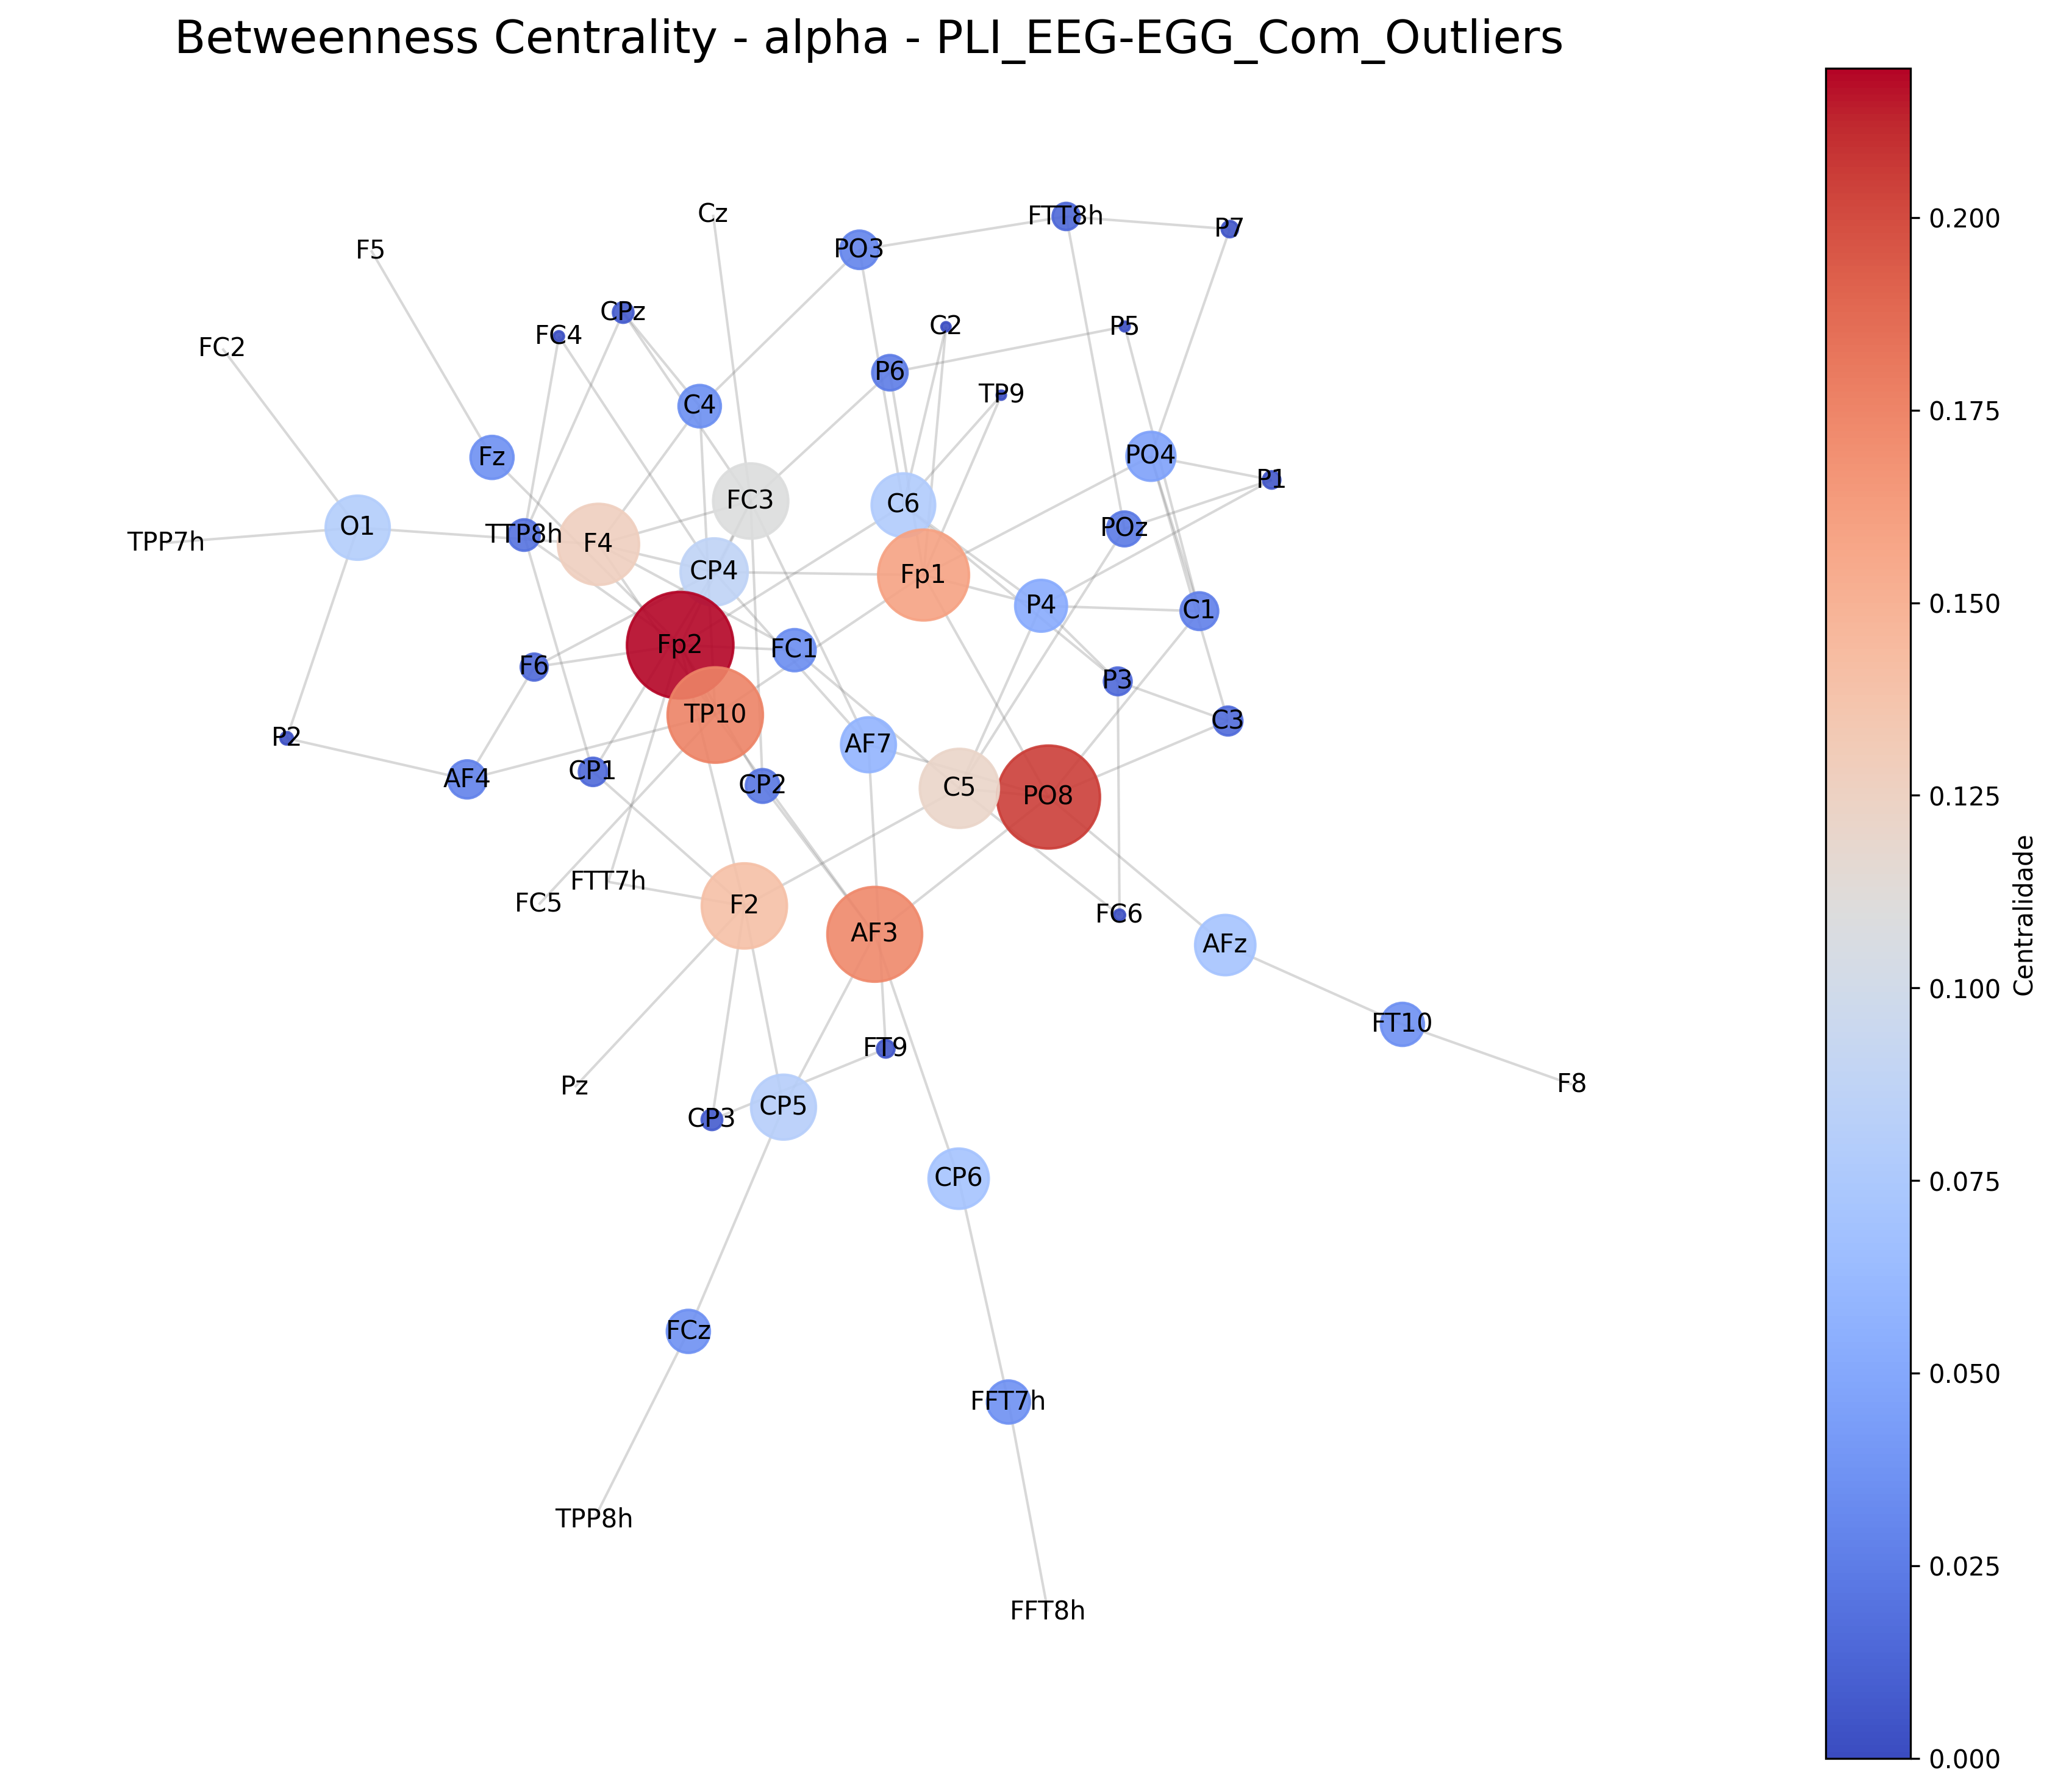
\includegraphics[width=0.45\textwidth]{figs/7_bootstrap_results_analysis/3_centrality_graphs/Com_Outliers/Betweenness_Centrality__alpha__PLI_EEGEGG_Com_Outliers.png}
    }
    \hfill
    \subfloat[\small \textbf{Sem Outliers:} Hierarquia – 1. \textbf{Fp2}; 2. \textbf{PO8, C6, F4, O1}; 3. \textbf{Fp1, TP9}; 4. \textbf{AF3, FC3, F2, TP10}.]{%
        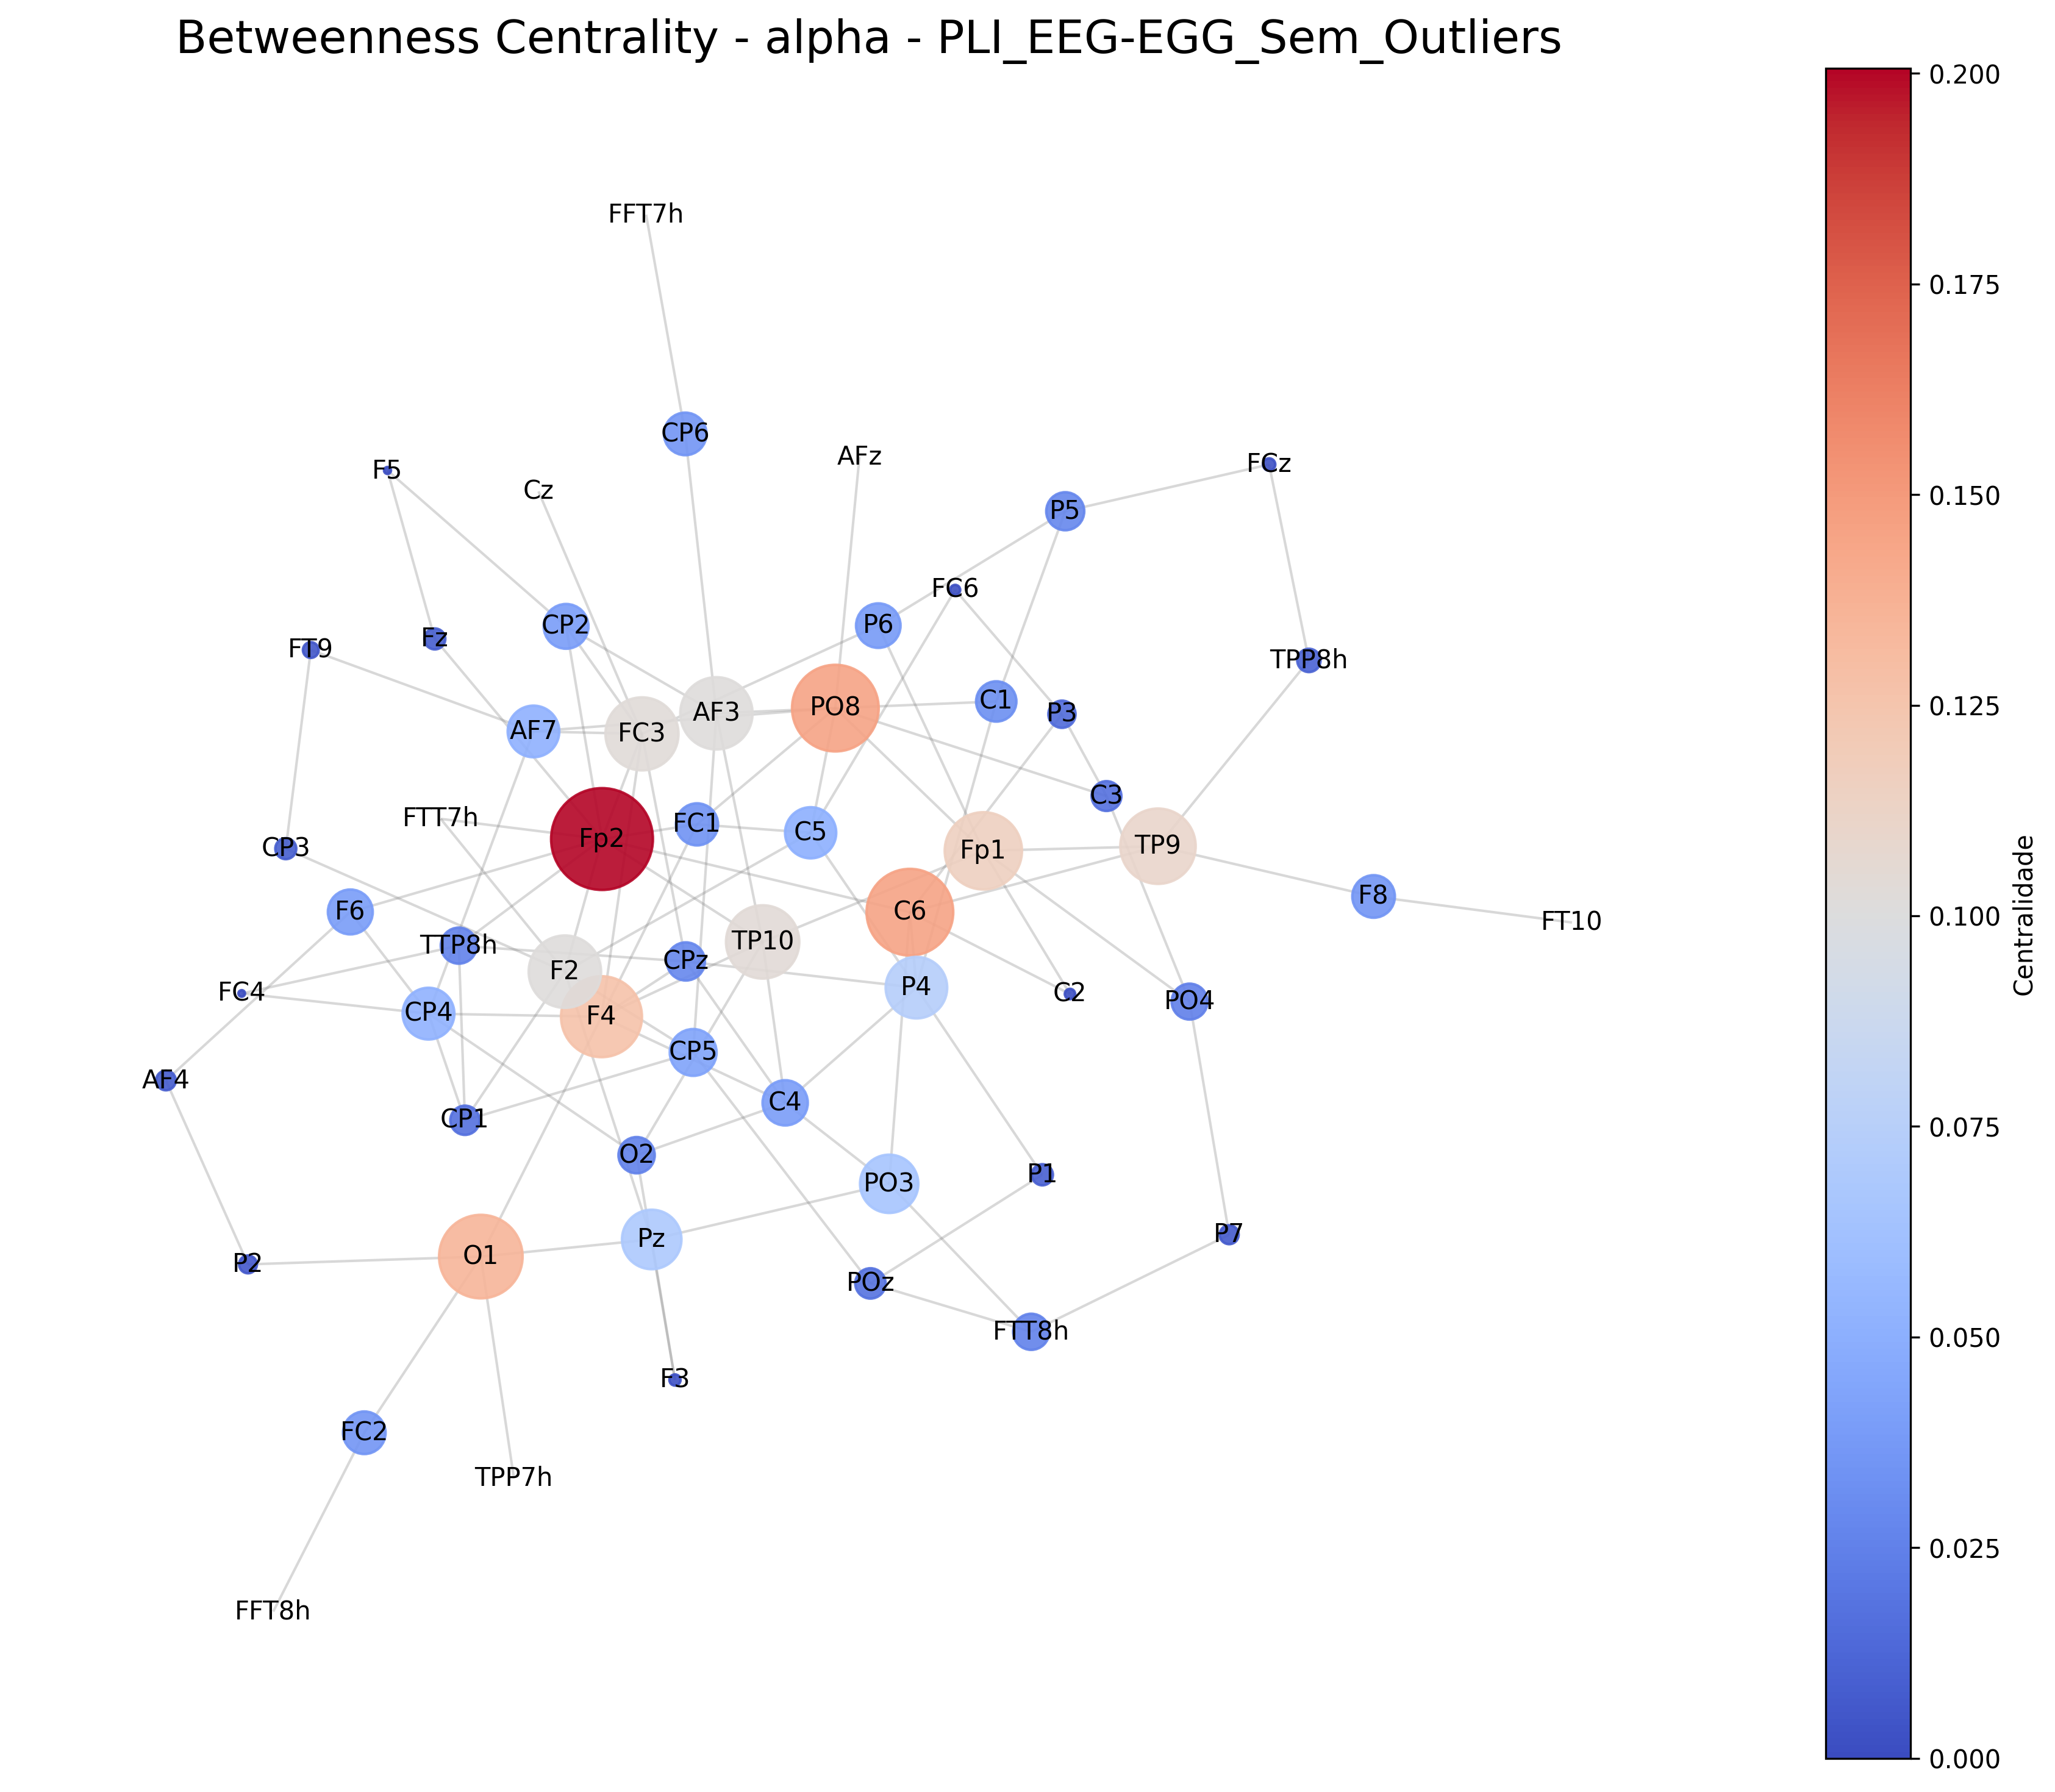
\includegraphics[width=0.45\textwidth]{figs/7_bootstrap_results_analysis/3_centrality_graphs/Sem_Outliers/Betweenness_Centrality__alpha__PLI_EEGEGG_Sem_Outliers.png}
    }
    \caption{\small \textbf{Betweenness Centrality – Banda Alpha (8--13 Hz):} A importância dos canais na mediação dos caminhos da rede é destacada pelos nós com cores mais quentes (vermelho intenso) e maiores tamanhos.}
    \label{fig:betweenness_alpha}
\end{figure}

\subsubsection{Degree Centrality}
\begin{figure}[H]
    \centering
    \subfloat[\small \textbf{Com Outliers:} Hierarquia – 1. \textbf{Fp2}; 2. \textbf{FC3, Fp1}; 3. \textbf{CP4, TP10, PO8, F2}; 4. \textbf{F4, C6, P4, C5}.]{%
        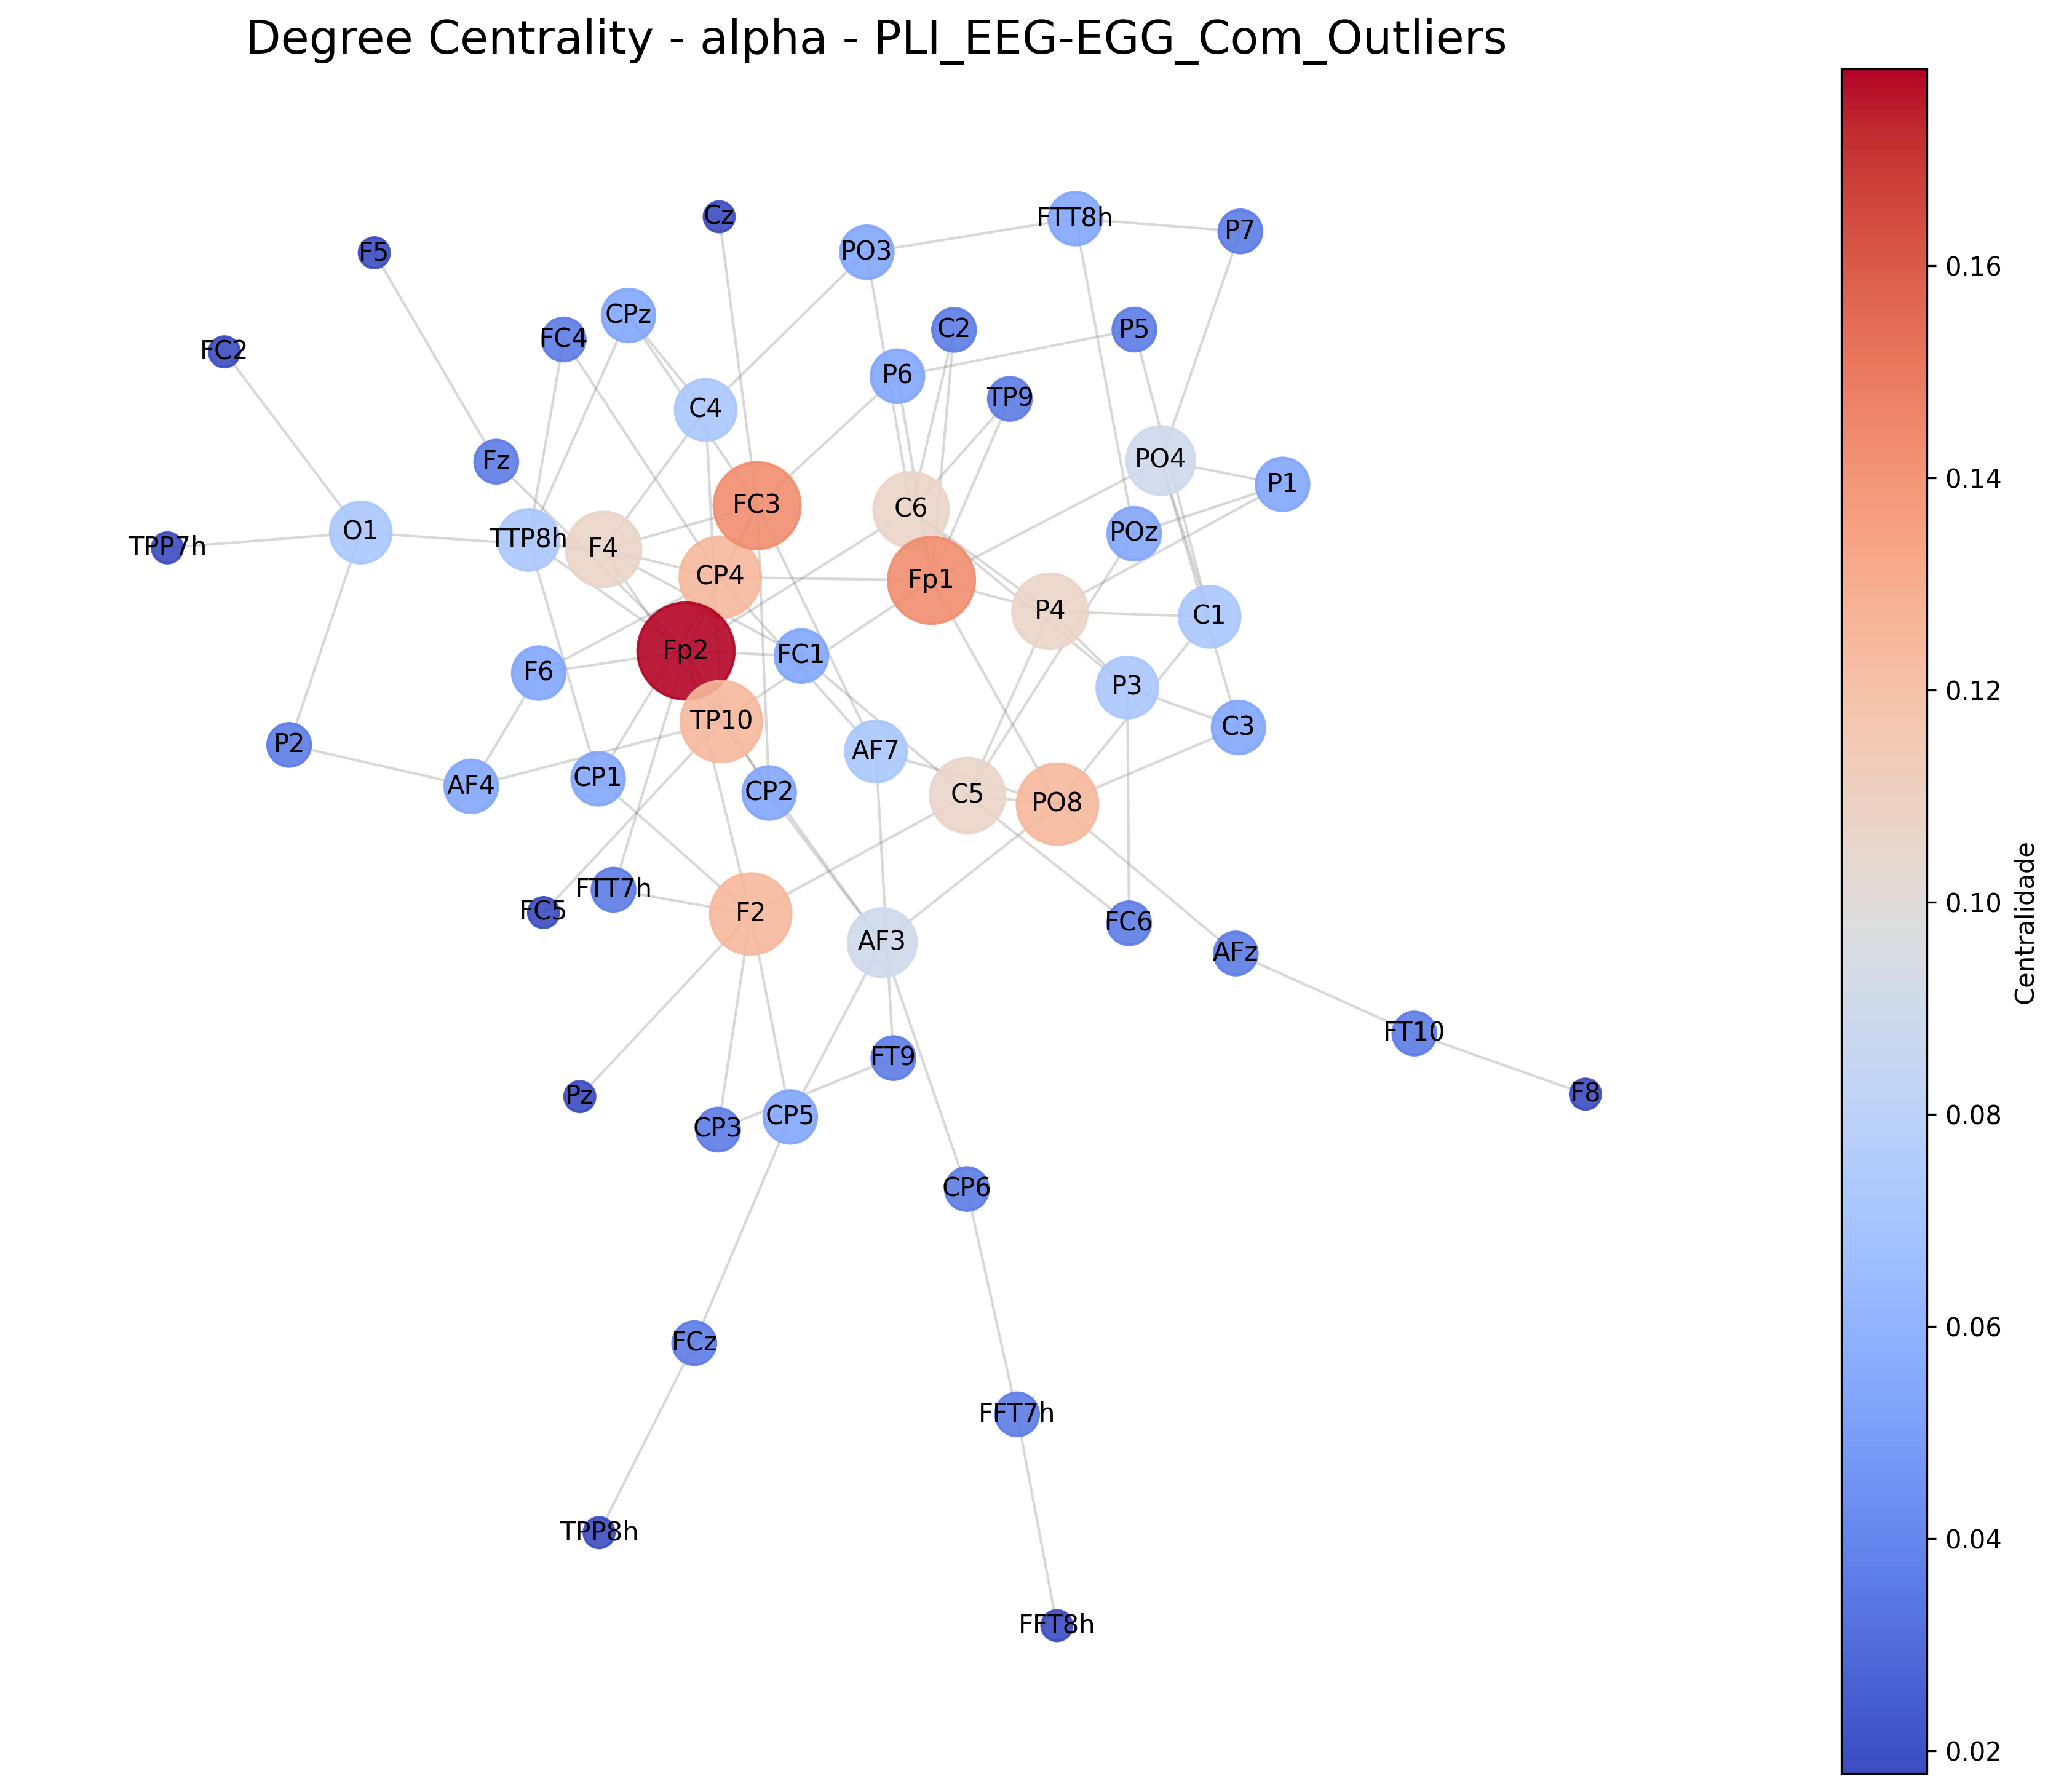
\includegraphics[width=0.45\textwidth]{figs/7_bootstrap_results_analysis/3_centrality_graphs/Com_Outliers/Degree_Centrality__alpha__PLI_EEGEGG_Com_Outliers.png}
    }
    \hfill
    \subfloat[\small \textbf{Sem Outliers:} Hierarquia – 1. \textbf{Fp2}; 2. \textbf{PO8}; 3. \textbf{FC3, F2, F4}; 4. \textbf{C6, Fp1, P4, C4, CP4}.]{%
        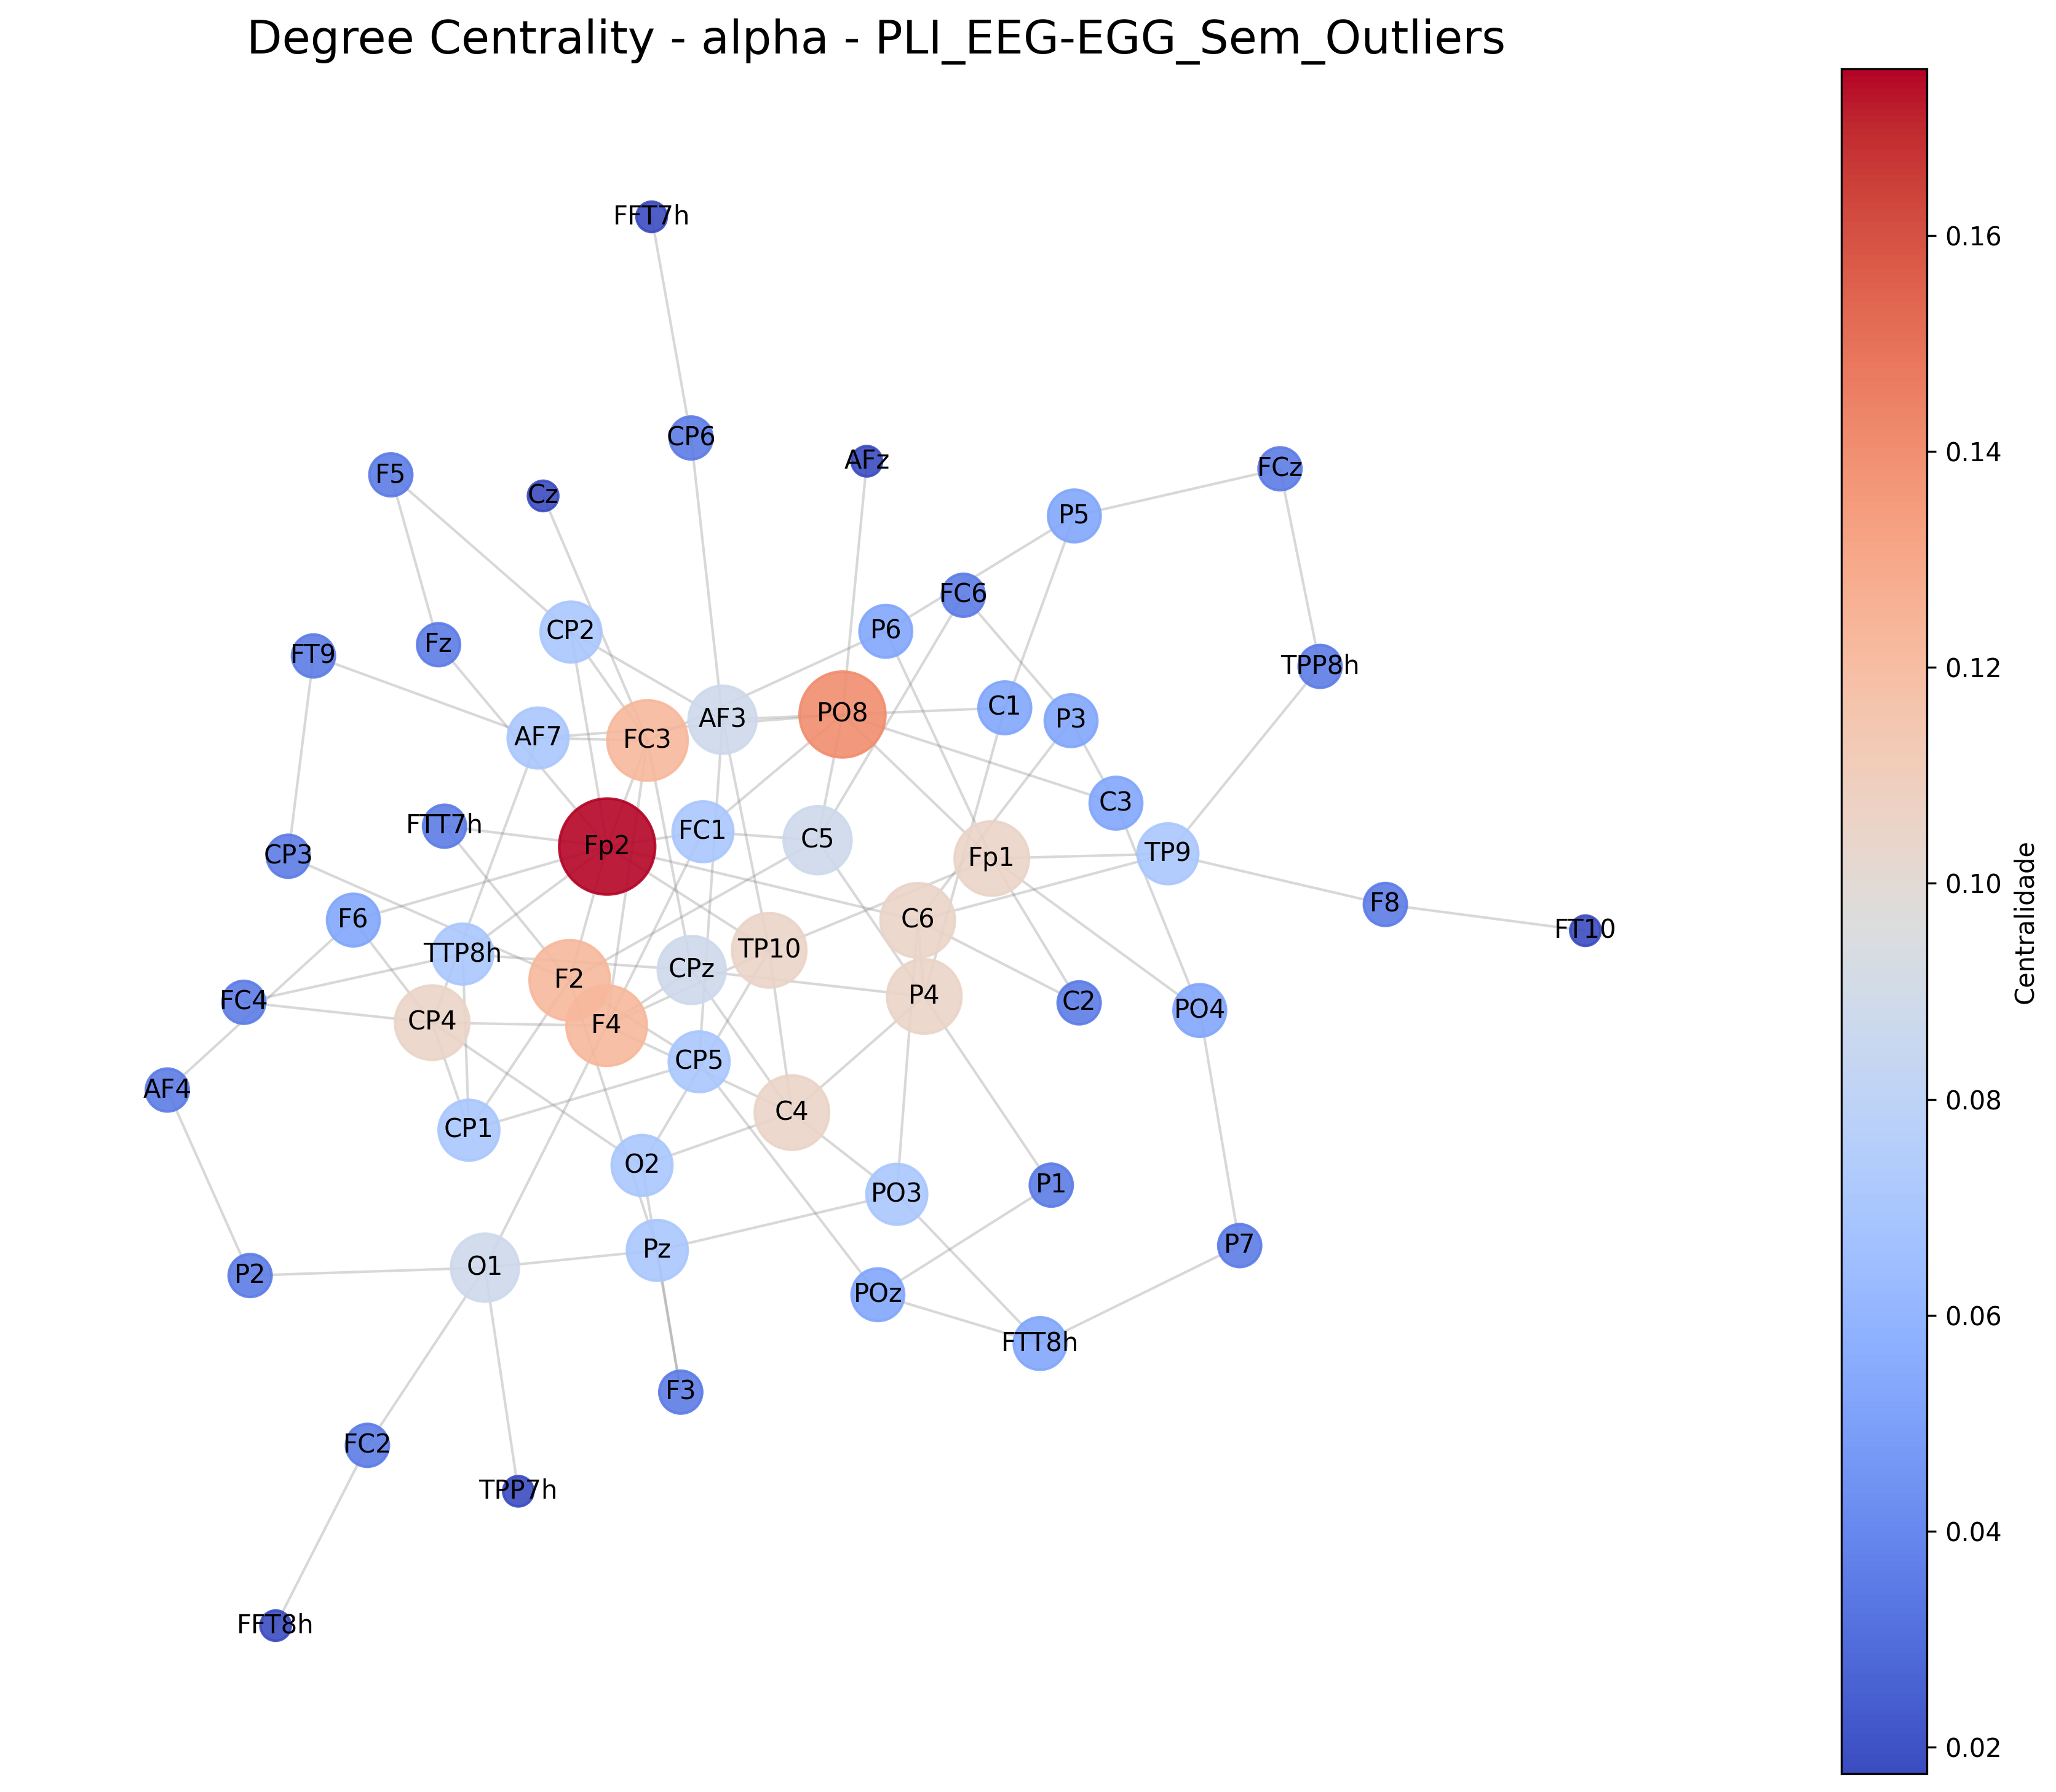
\includegraphics[width=0.45\textwidth]{figs/7_bootstrap_results_analysis/3_centrality_graphs/Sem_Outliers/Degree_Centrality__alpha__PLI_EEGEGG_Sem_Outliers.png}
    }
    \caption{\small \textbf{Degree Centrality – Banda Alpha (8--13 Hz):} Os nós com maior número de conexões diretas aparecem destacados, evidenciando a hierarquia dos canais na rede.}
    \label{fig:degree_alpha}
\end{figure}

\subsubsection{Eigenvector Centrality}
\begin{figure}[H]
    \centering
    \subfloat[\small \textbf{Com Outliers:} Hierarquia – 1. \textbf{Fp2}; 2. \textbf{FC3}; 3. \textbf{CP4, F4, TP10, Fp1}; 4. \textbf{PO8}.]{%
        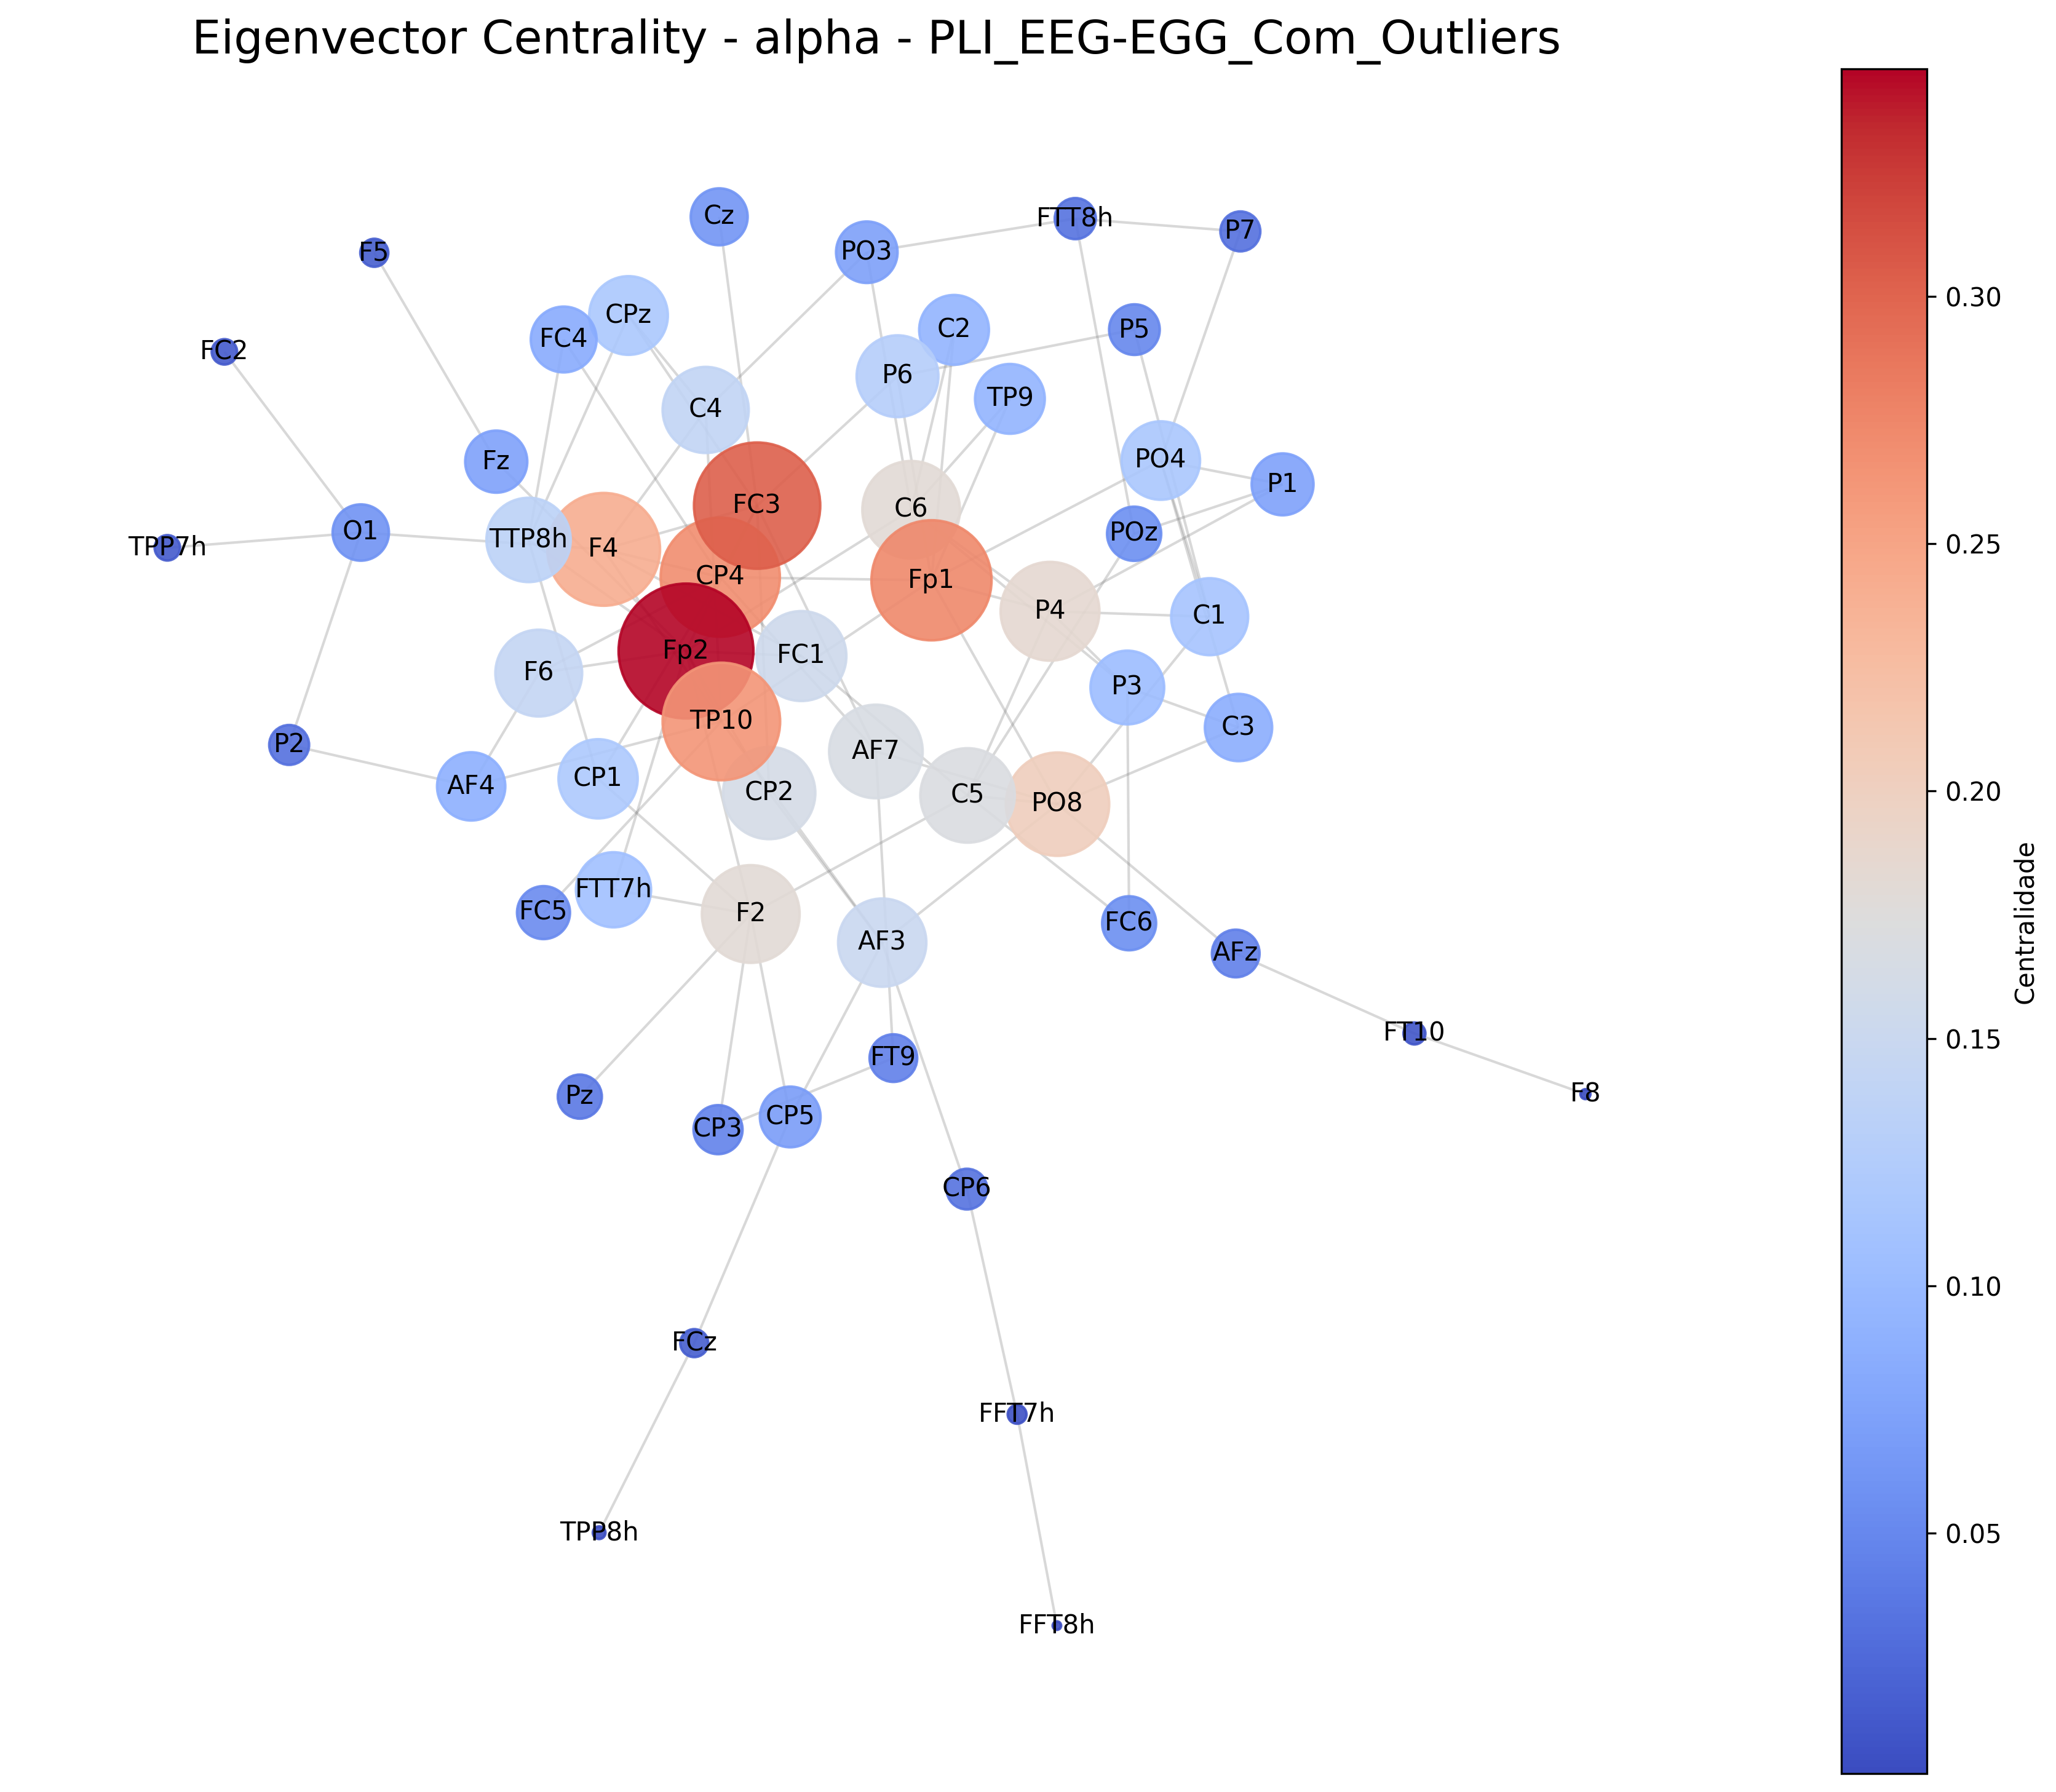
\includegraphics[width=0.45\textwidth]{figs/7_bootstrap_results_analysis/3_centrality_graphs/Com_Outliers/Eigenvector_Centrality__alpha__PLI_EEGEGG_Com_Outliers.png}
    }
    \hfill
    \subfloat[\small \textbf{Sem Outliers:} Hierarquia – 1. \textbf{Fp2}; 2. \textbf{F4}; 3. \textbf{FC3, TP10}; 4. \textbf{Cpz, C4}; 5. \textbf{PO8, P4, FC1, F2, P4}.]{%
        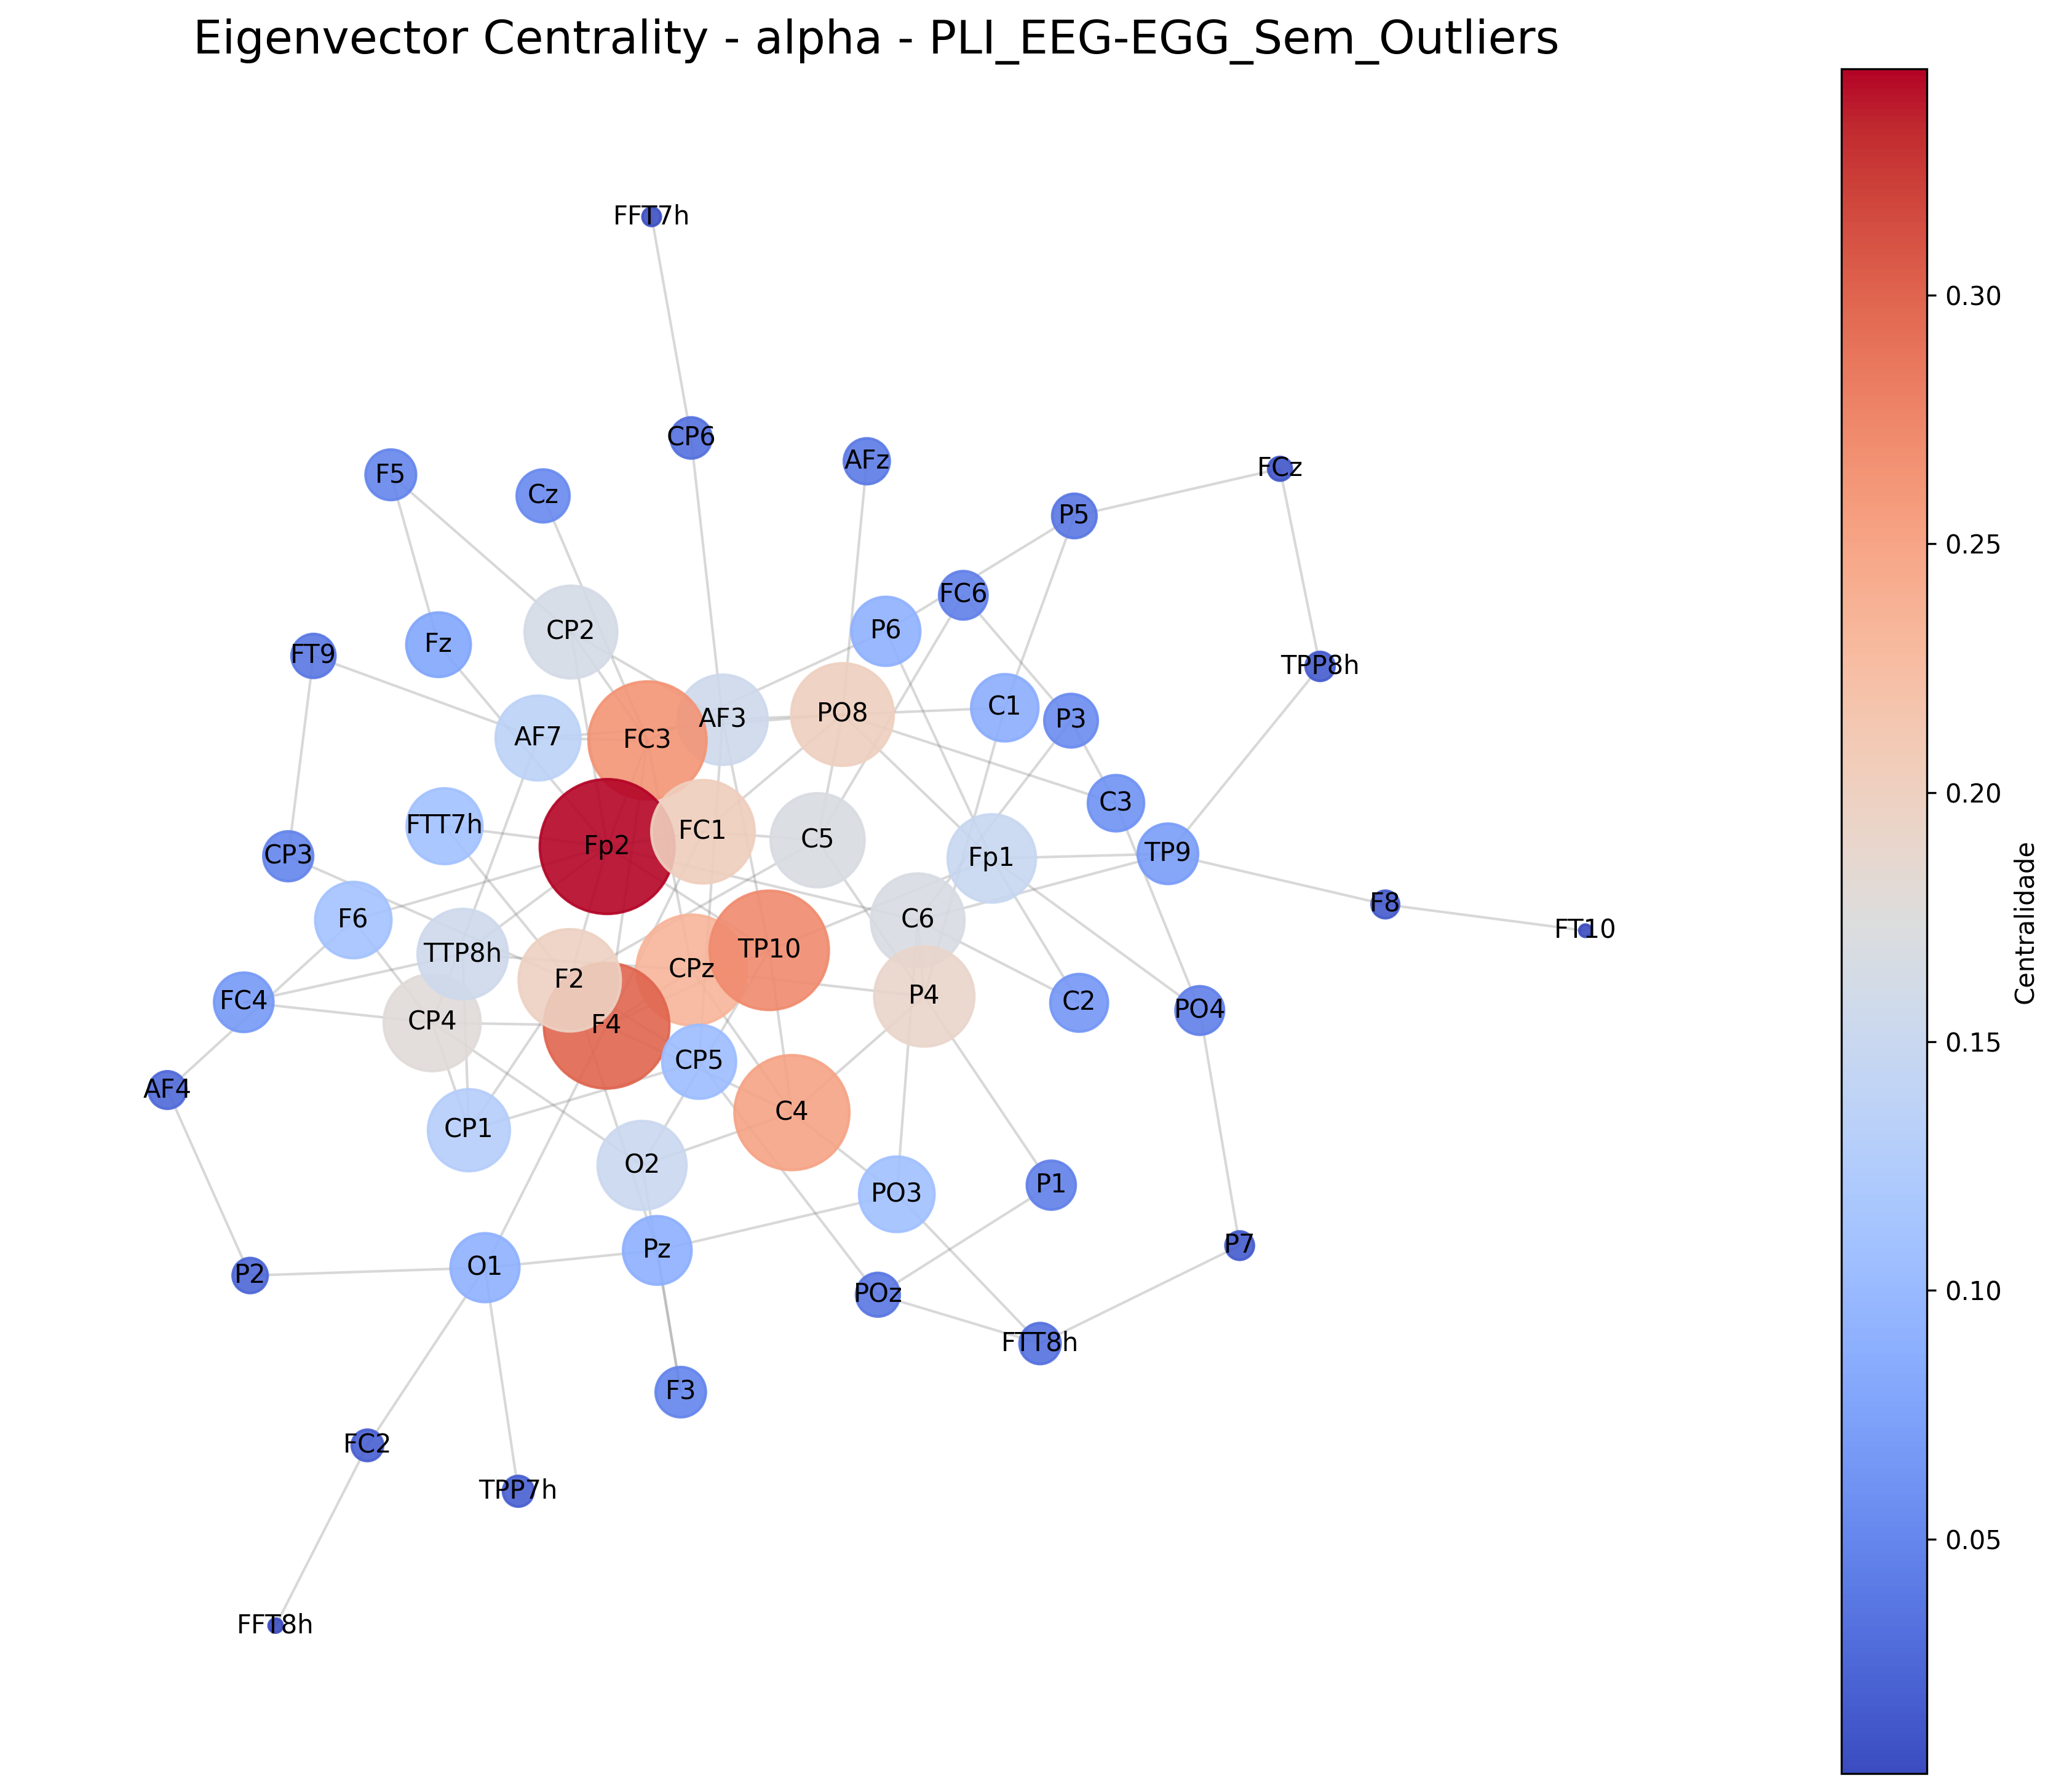
\includegraphics[width=0.45\textwidth]{figs/7_bootstrap_results_analysis/3_centrality_graphs/Sem_Outliers/Eigenvector_Centrality__alpha__PLI_EEGEGG_Sem_Outliers.png}
    }
    \caption{\small \textbf{Eigenvector Centrality – Banda Alpha (8--13 Hz):} A influência dos canais é demonstrada pela hierarquia dos nós, com os valores mais elevados destacados em tons intensos.}
    \label{fig:eigenvector_alpha}
\end{figure}

\subsection{Banda Beta (13--30 Hz)}

\subsubsection{Betweenness Centrality}
\begin{figure}[H]
    \centering
    \subfloat[\small \textbf{Com Outliers:} Hierarquia – 1. \textbf{CP5, F5}; 2. \textbf{CP1}; 3. \textbf{F2, POz}; 4. \textbf{TPP7h}.]{%
        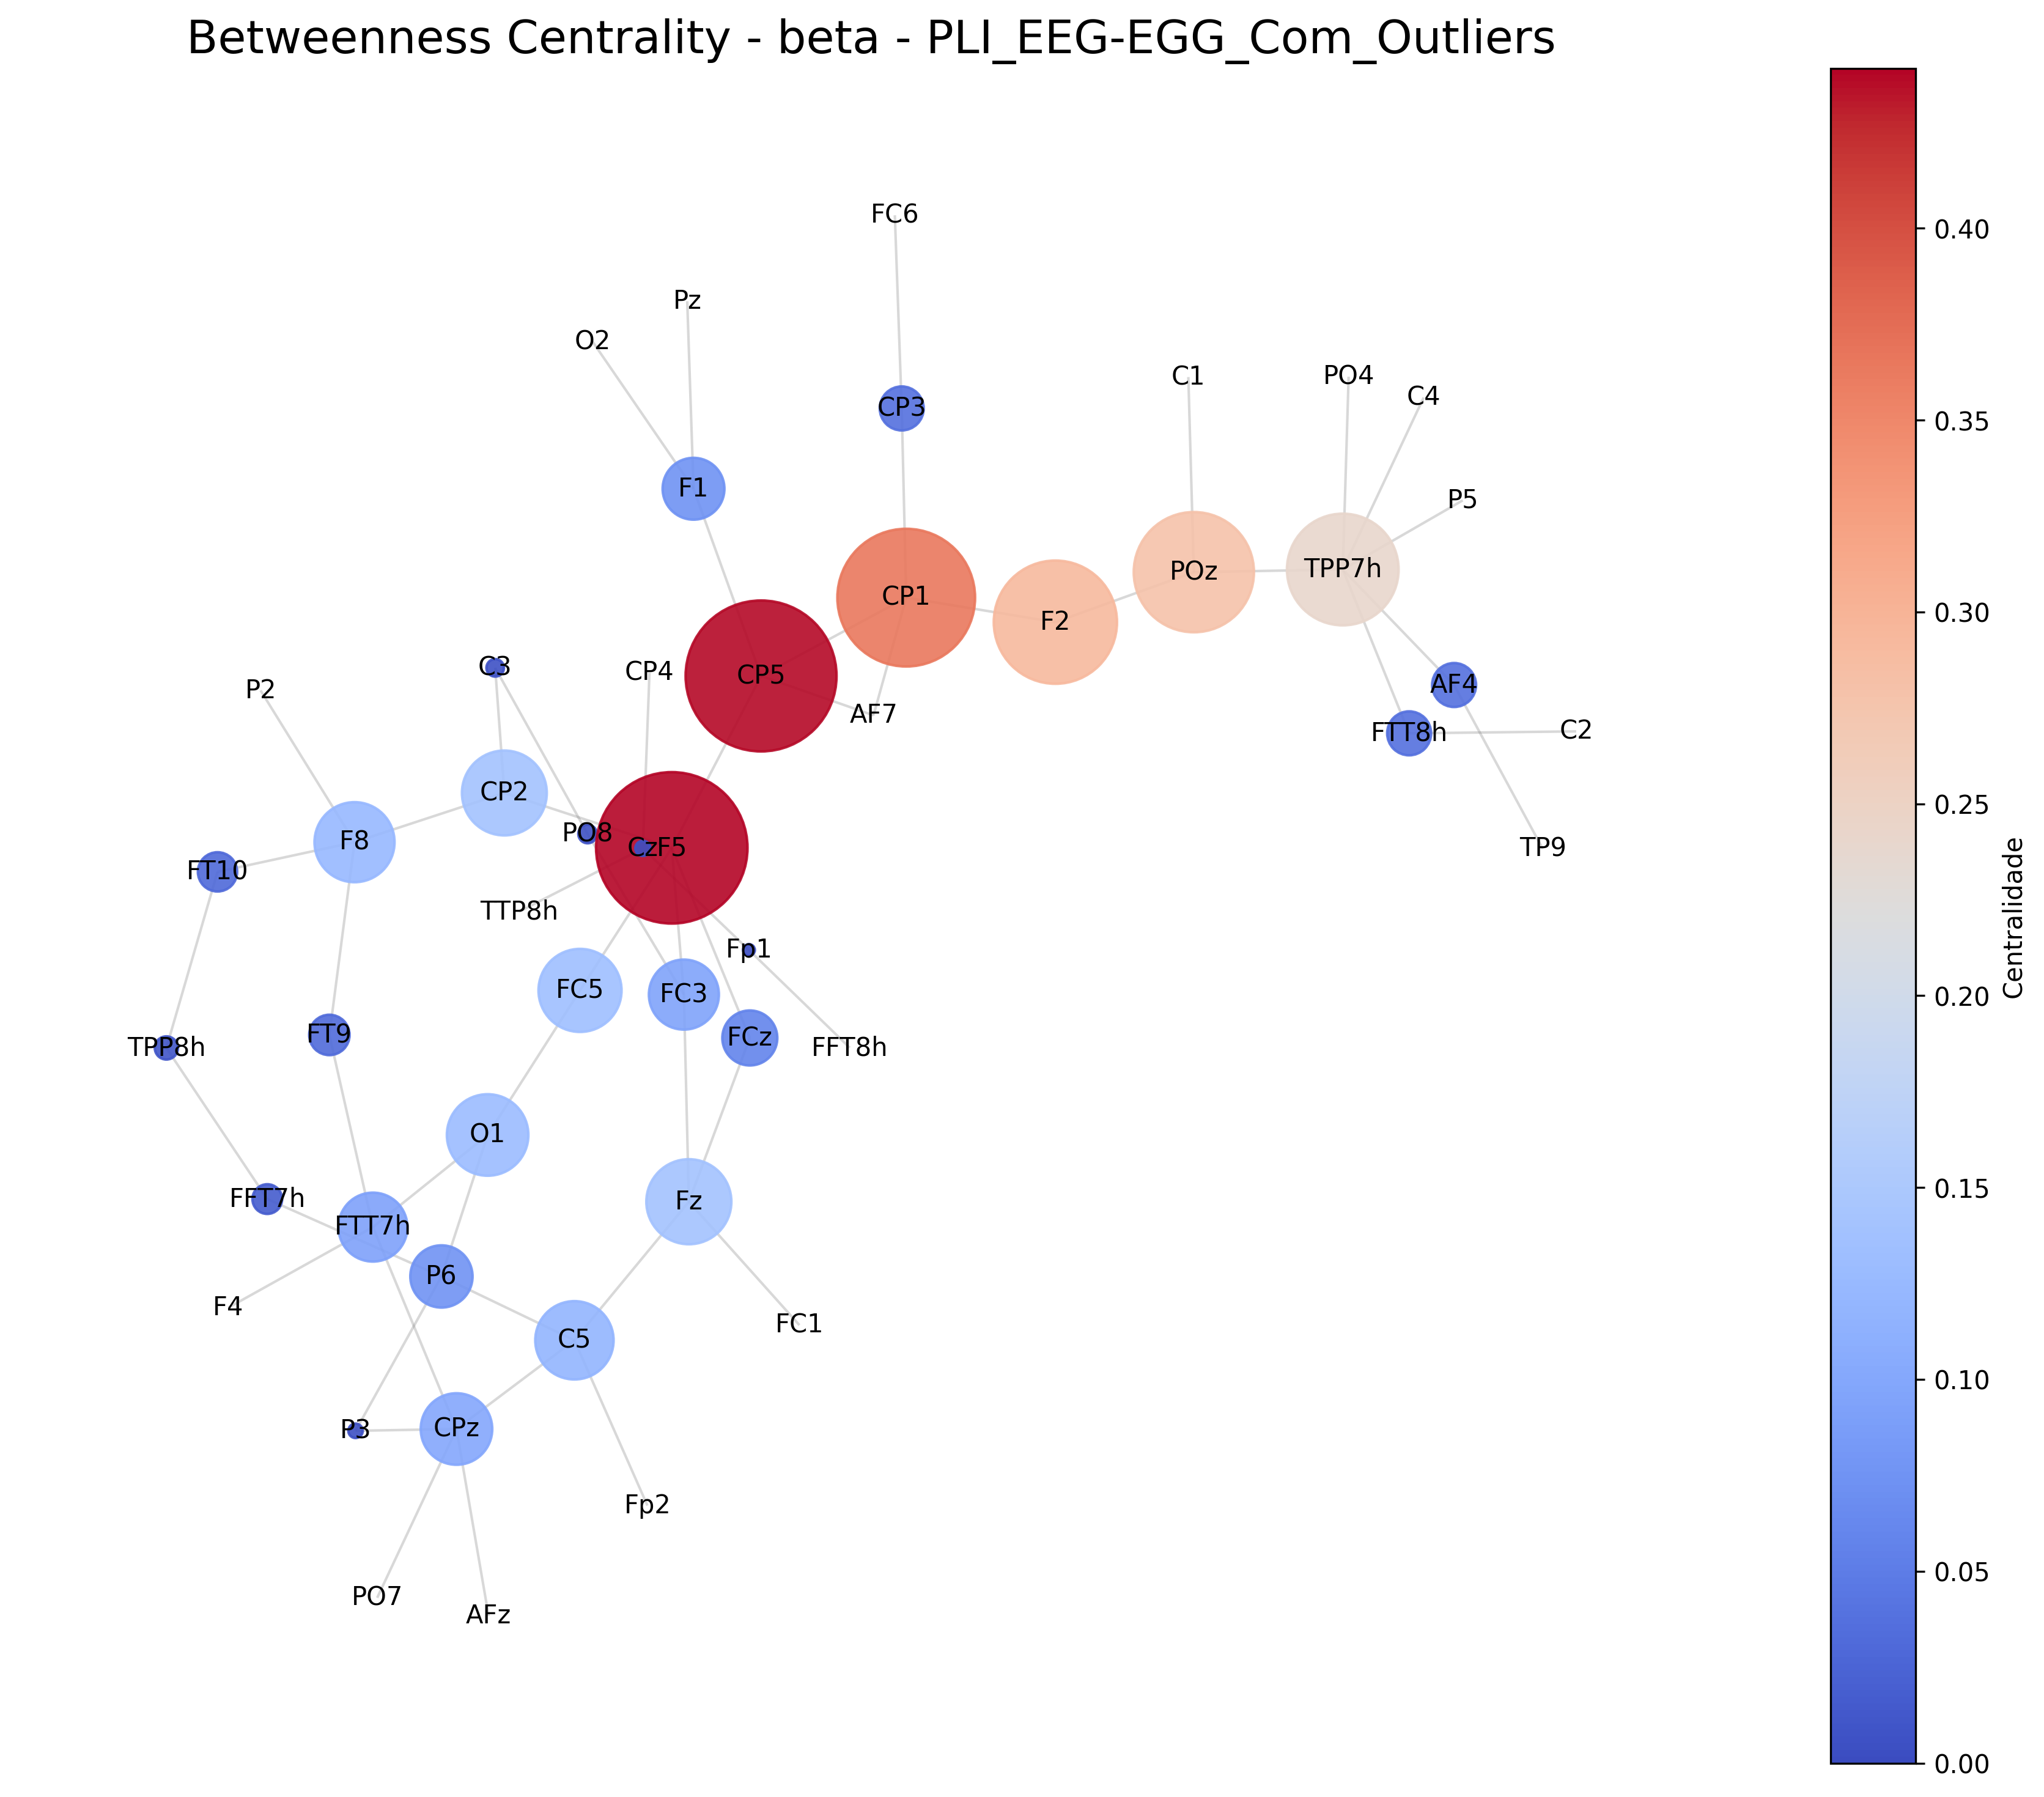
\includegraphics[width=0.45\textwidth]{figs/7_bootstrap_results_analysis/3_centrality_graphs/Com_Outliers/Betweenness_Centrality__beta__PLI_EEGEGG_Com_Outliers.png}
    }
    \hfill
    \subfloat[\small \textbf{Sem Outliers:} Hierarquia – 1. \textbf{TPP7h}; 2. \textbf{CP5, F5, CP2}; 3. \textbf{FFT7h}; 4. \textbf{TTP8h}; 5. \textbf{CPz}; 6. \textbf{P6}.]{%
        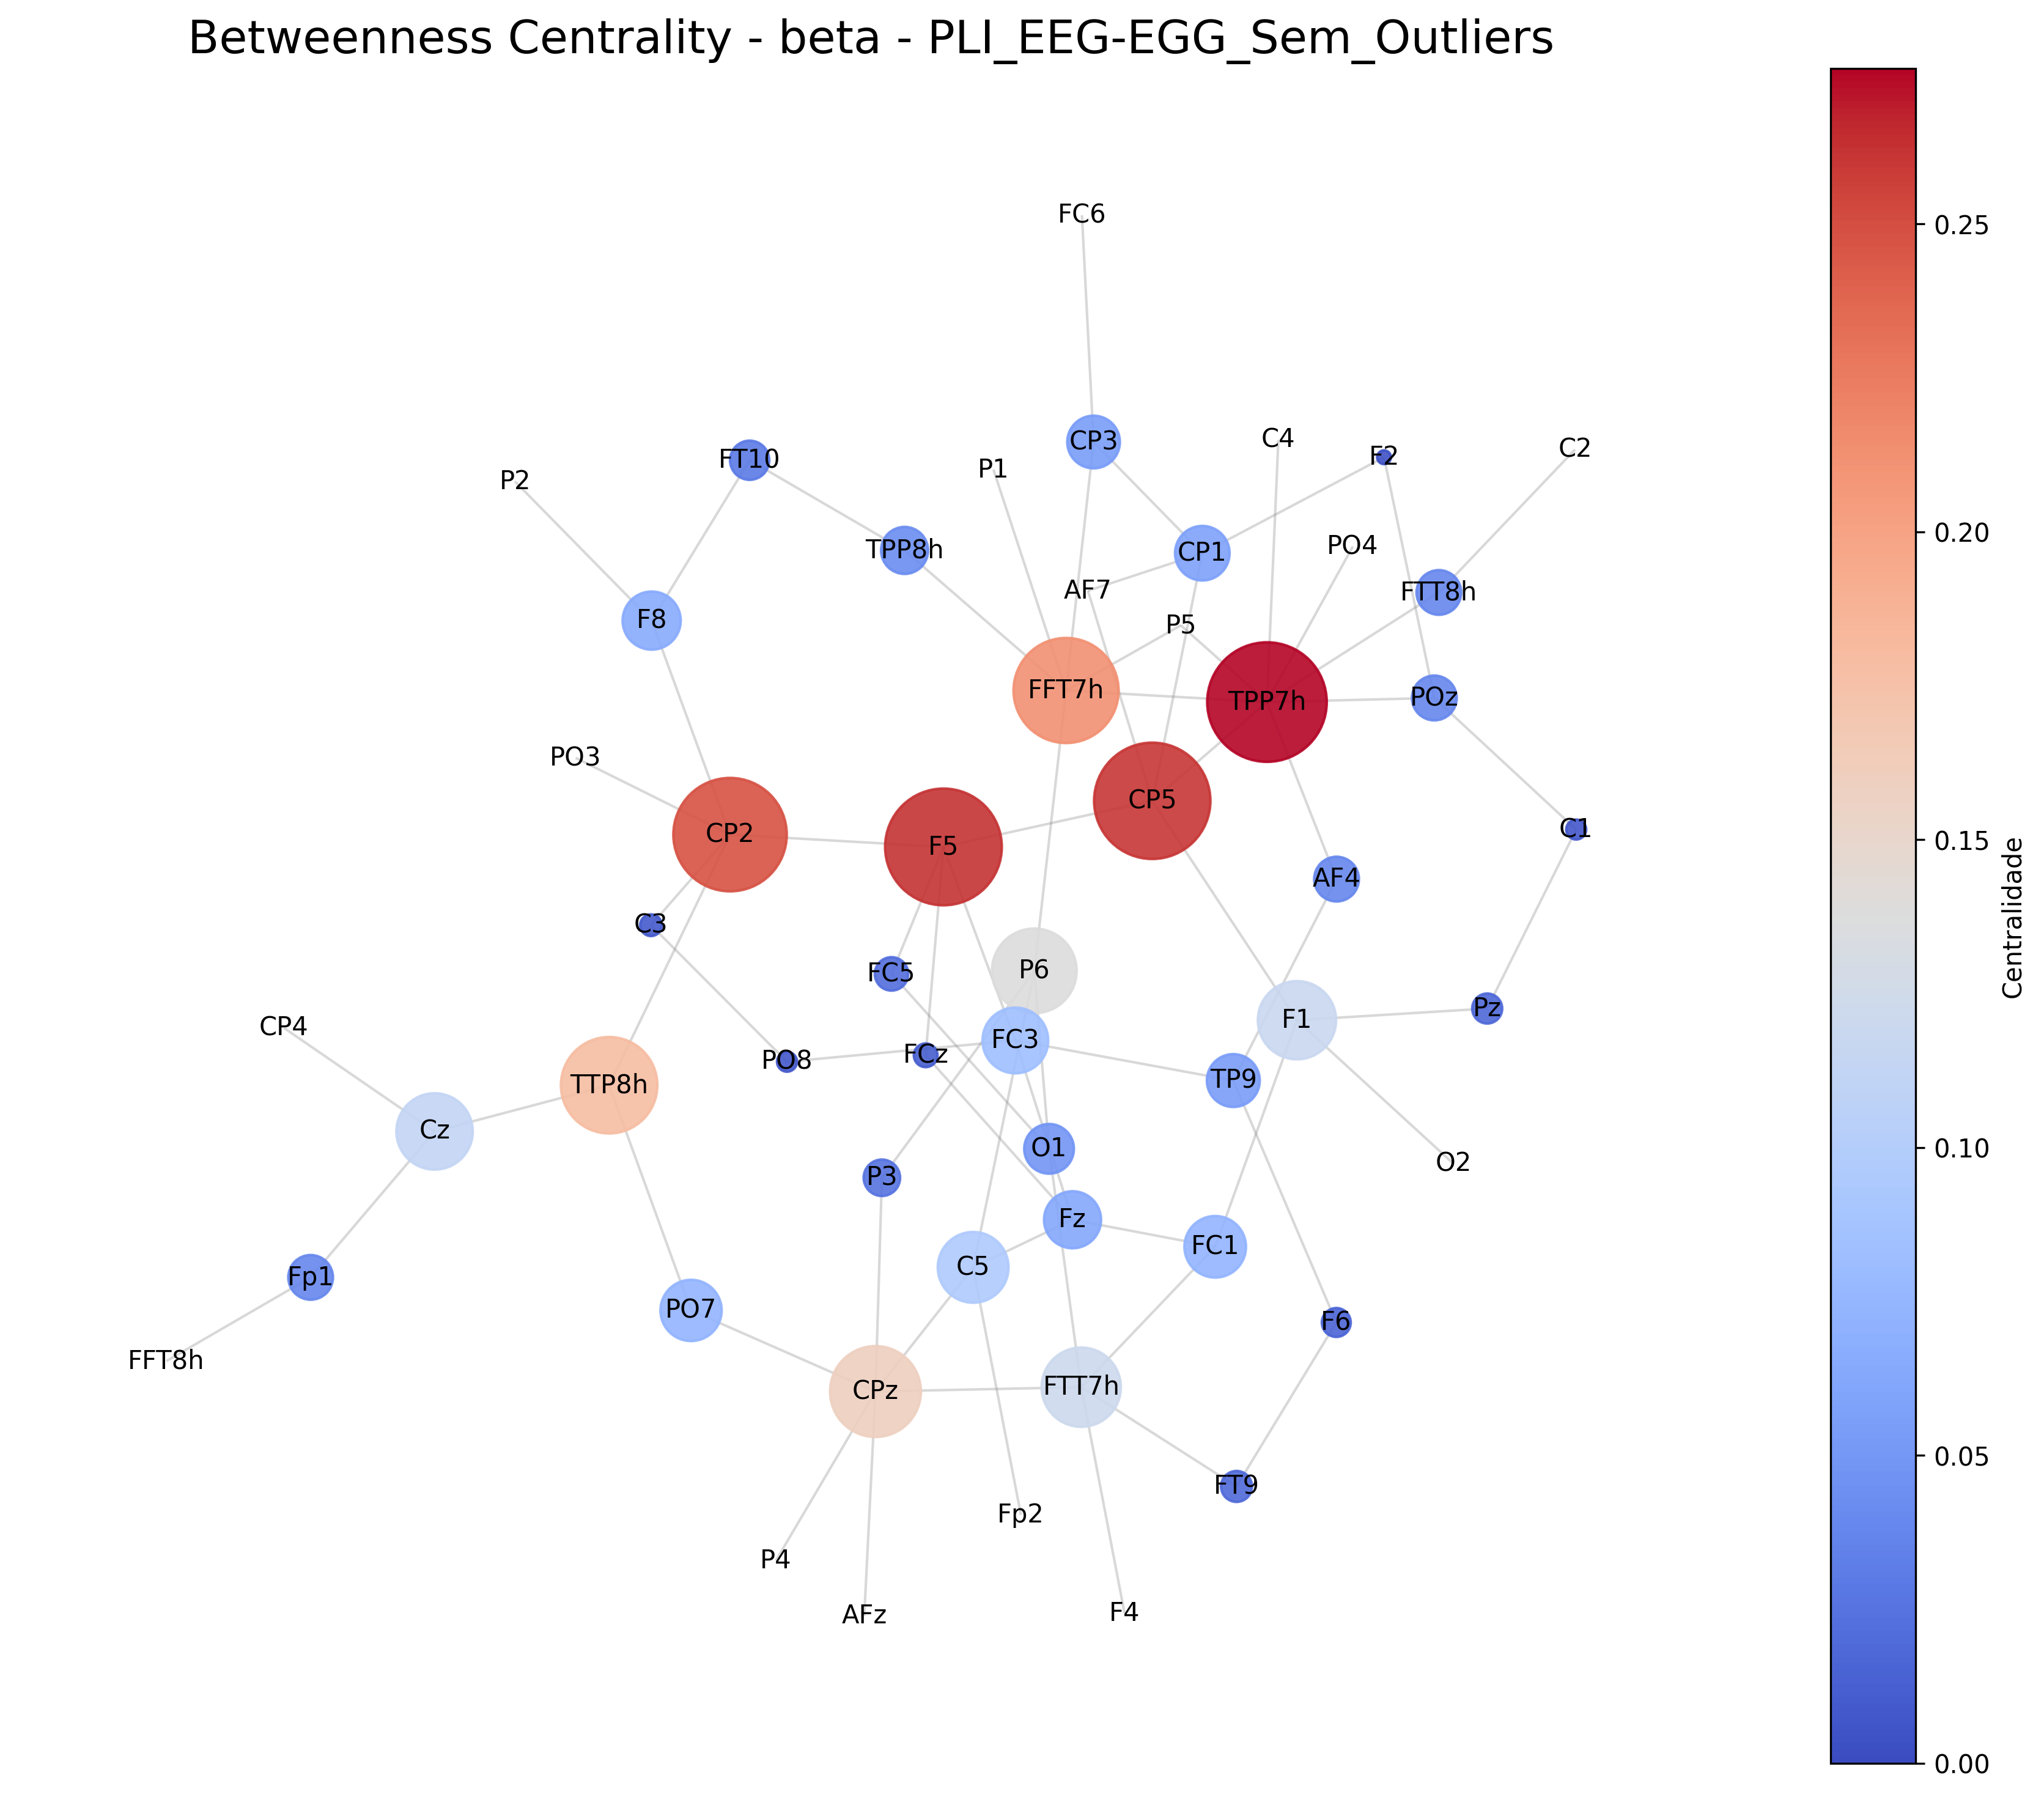
\includegraphics[width=0.45\textwidth]{figs/7_bootstrap_results_analysis/3_centrality_graphs/Sem_Outliers/Betweenness_Centrality__beta__PLI_EEGEGG_Sem_Outliers.png}
    }
    \caption{\small \textbf{Betweenness Centrality – Banda Beta (13--30 Hz):} A rede beta evidencia canais-chave, com destaque para \textbf{TPP7h} na versão sem outliers.}
    \label{fig:betweenness_beta}
\end{figure}

\subsubsection{Degree Centrality}
\begin{figure}[H]
    \centering
    \subfloat[\small \textbf{Com Outliers:} Hierarquia – 1. \textbf{TPP7h}; 2. \textbf{F5, CPz}; 3. \textbf{CP1, CP5, F8, FTT7h, P6, C5, Fz}.]{%
        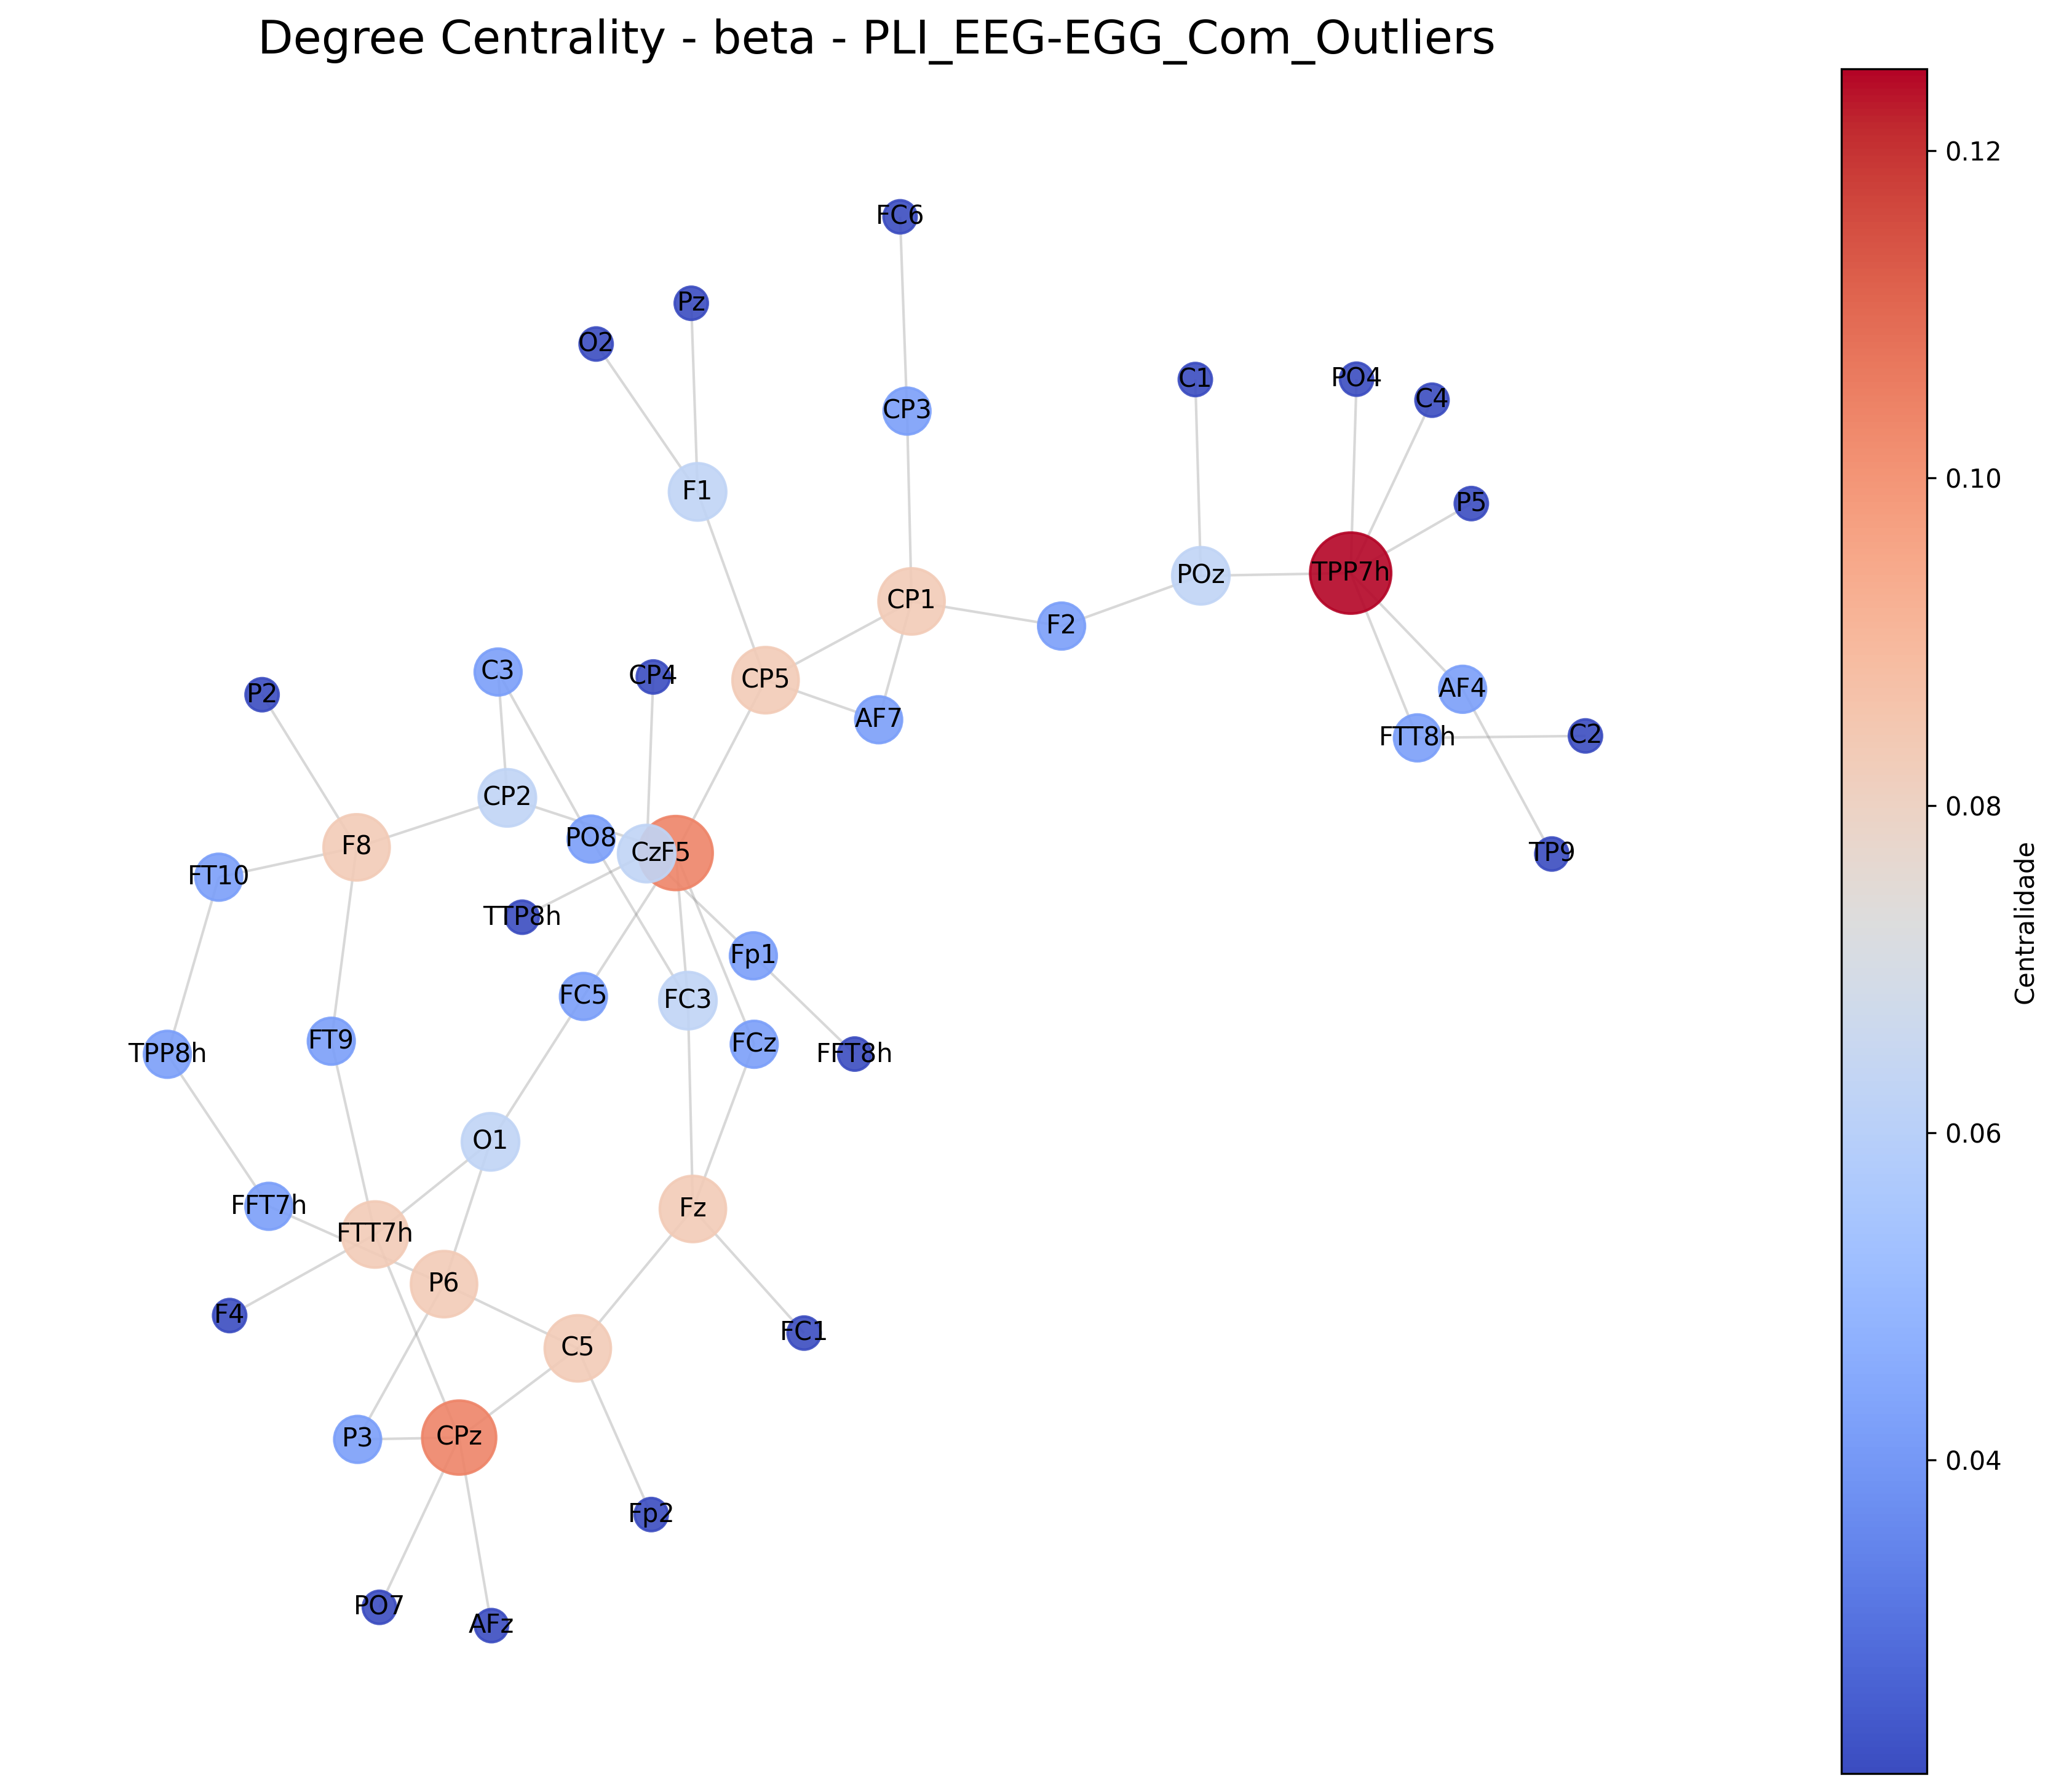
\includegraphics[width=0.45\textwidth]{figs/7_bootstrap_results_analysis/3_centrality_graphs/Com_Outliers/Degree_Centrality__beta__PLI_EEGEGG_Com_Outliers.png}
    }
    \hfill
    \subfloat[\small \textbf{Sem Outliers:} Hierarquia – 1. \textbf{TPP7h}; 2. \textbf{FTT7h, CPz}; 3. \textbf{CP5, F5, CP2, FTT7h}.]{%
        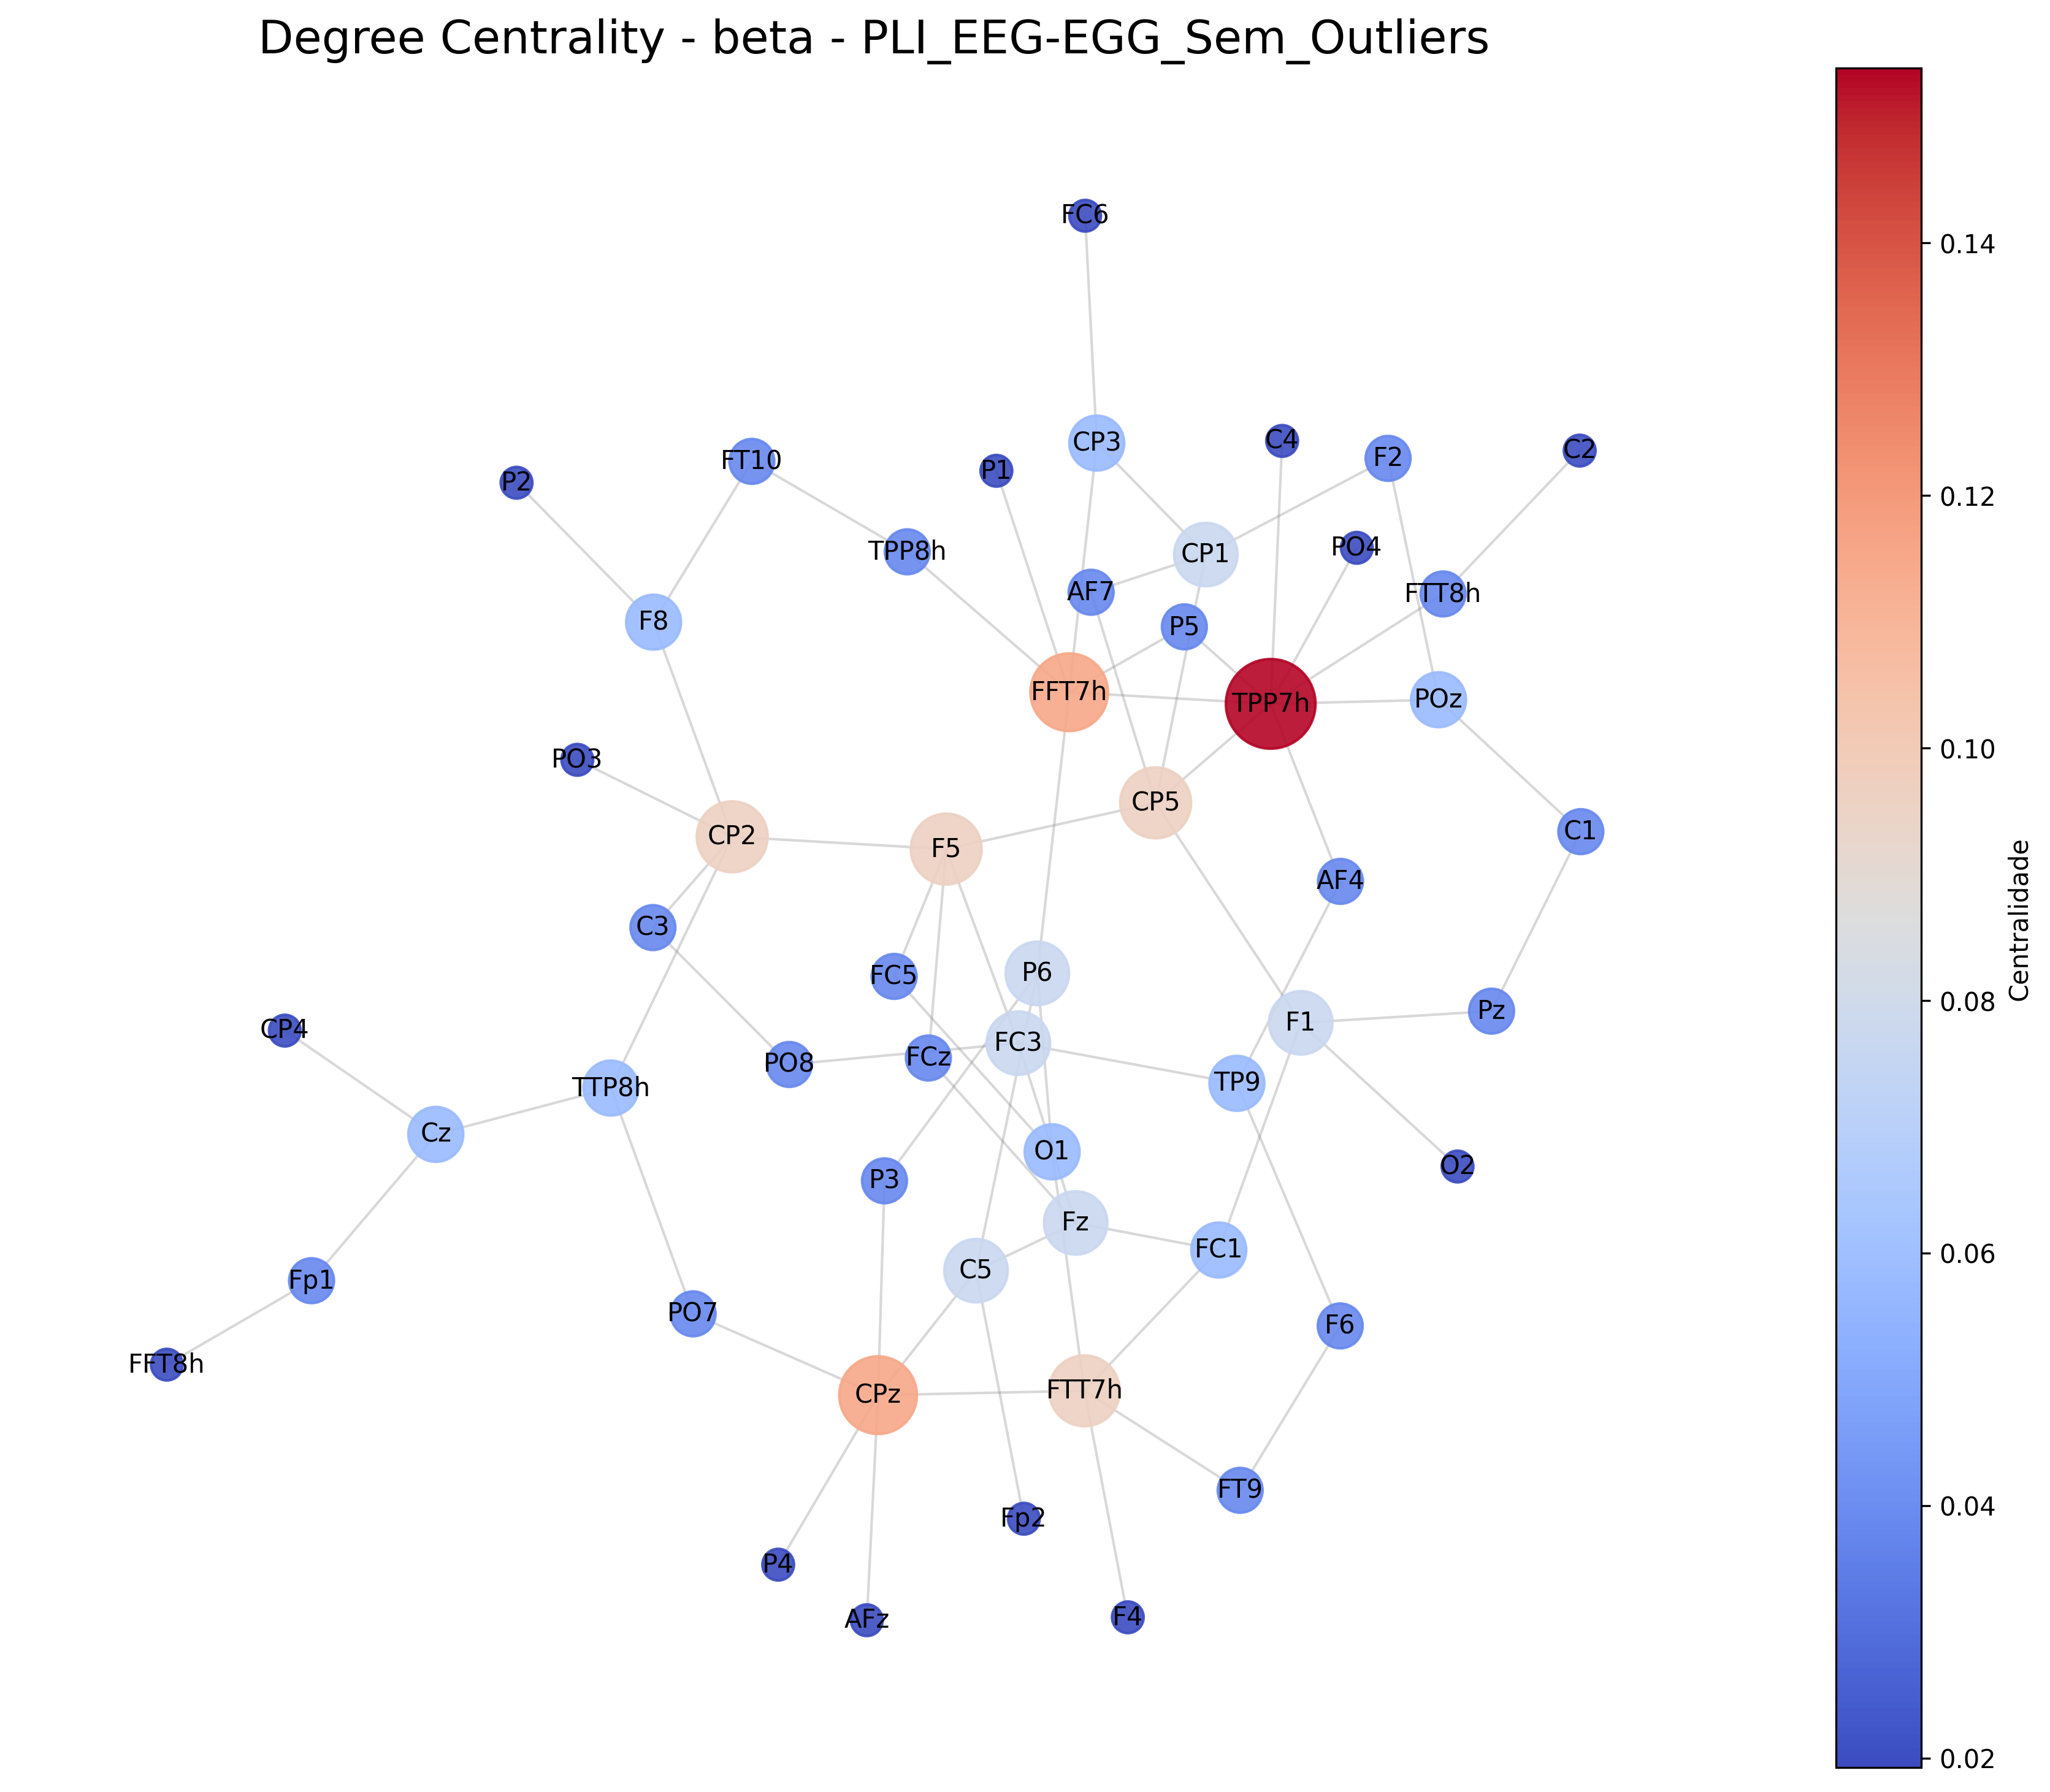
\includegraphics[width=0.45\textwidth]{figs/7_bootstrap_results_analysis/3_centrality_graphs/Sem_Outliers/Degree_Centrality__beta__PLI_EEGEGG_Sem_Outliers.png}
    }
    \caption{\small \textbf{Degree Centrality – Banda Beta (13--30 Hz):} A hierarquia na rede beta destaca consistentemente \textbf{TPP7h} como o hub principal, com pequenas variações na ordem dos outros canais entre os cenários.}
    \label{fig:degree_beta}
\end{figure}

\subsubsection{Eigenvector Centrality}
\begin{figure}[H]
    \centering
    \subfloat[\small \textbf{Com Outliers:} Hierarquia – 1. \textbf{F5}; 2. \textbf{C5, CPz}; 3. \textbf{P6, Fz}; 4. \textbf{CP5, O1, FFT7h, FC3}.]{%
        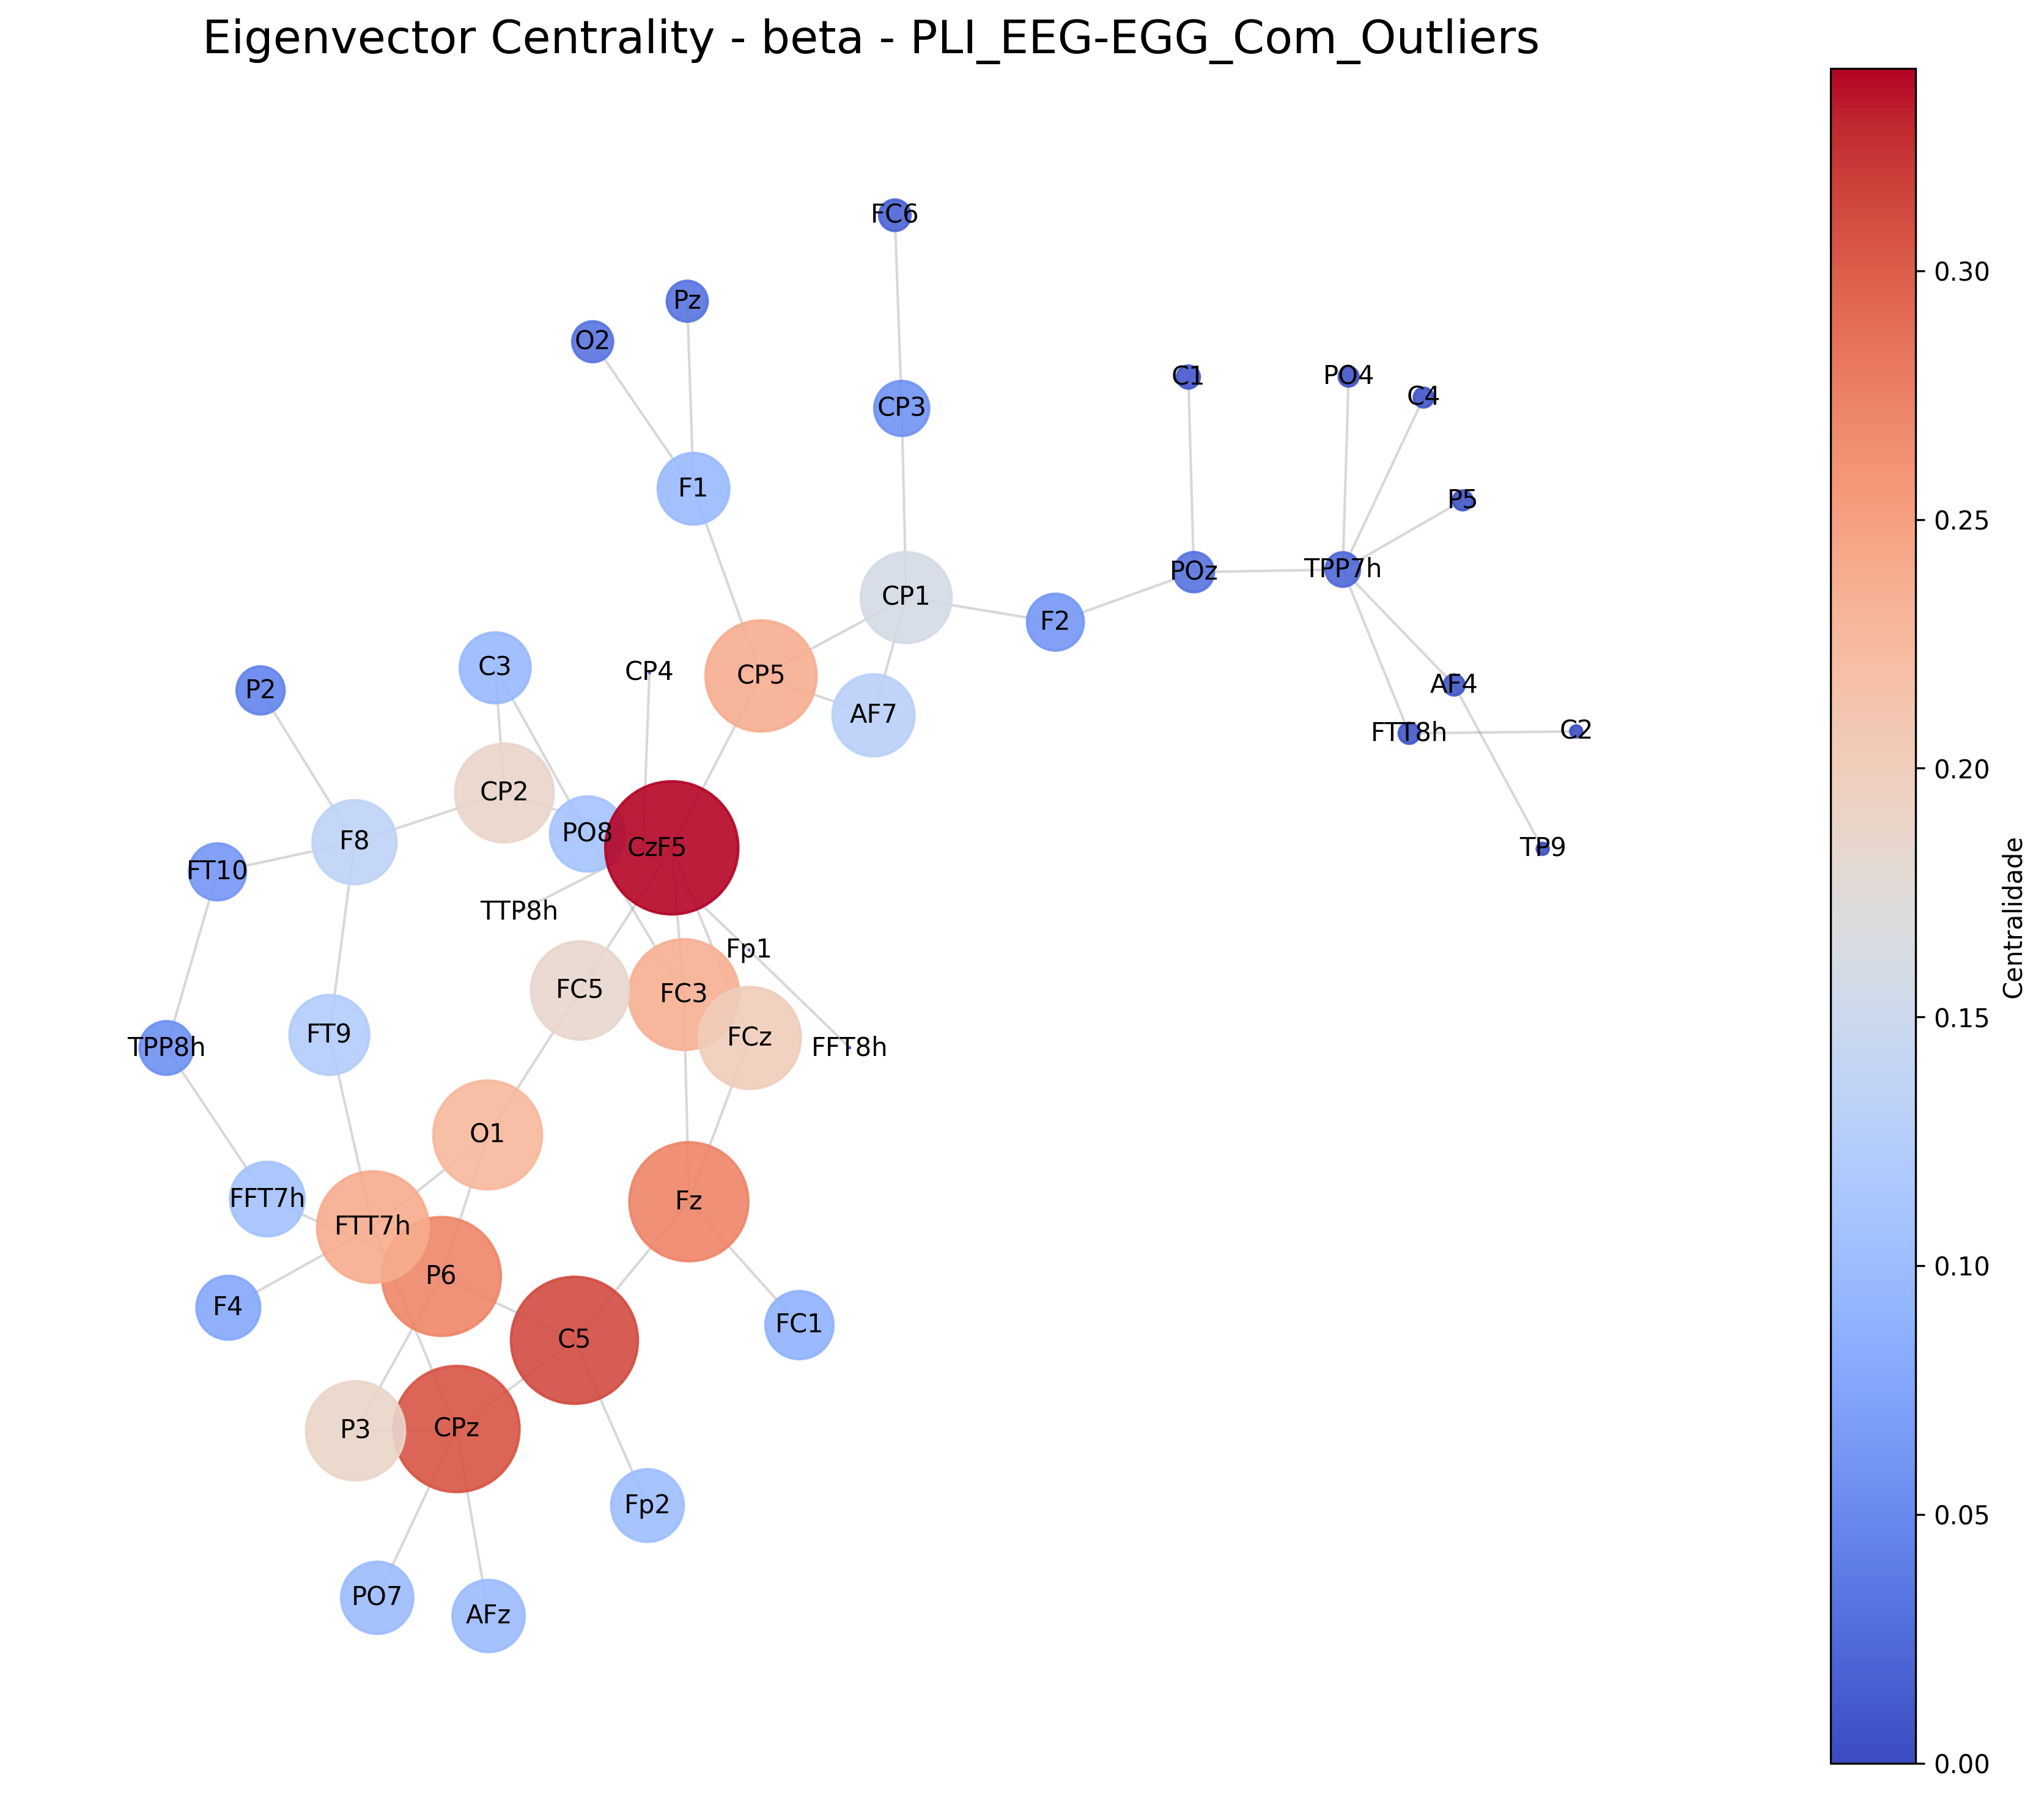
\includegraphics[width=0.45\textwidth]{figs/7_bootstrap_results_analysis/3_centrality_graphs/Com_Outliers/Eigenvector_Centrality__beta__PLI_EEGEGG_Com_Outliers.png}
    }
    \hfill
    \subfloat[\small \textbf{Sem Outliers:} Hierarquia – 1. \textbf{TPP7h}; 2. \textbf{FTT7h}; 3. \textbf{CP5}.]{%
        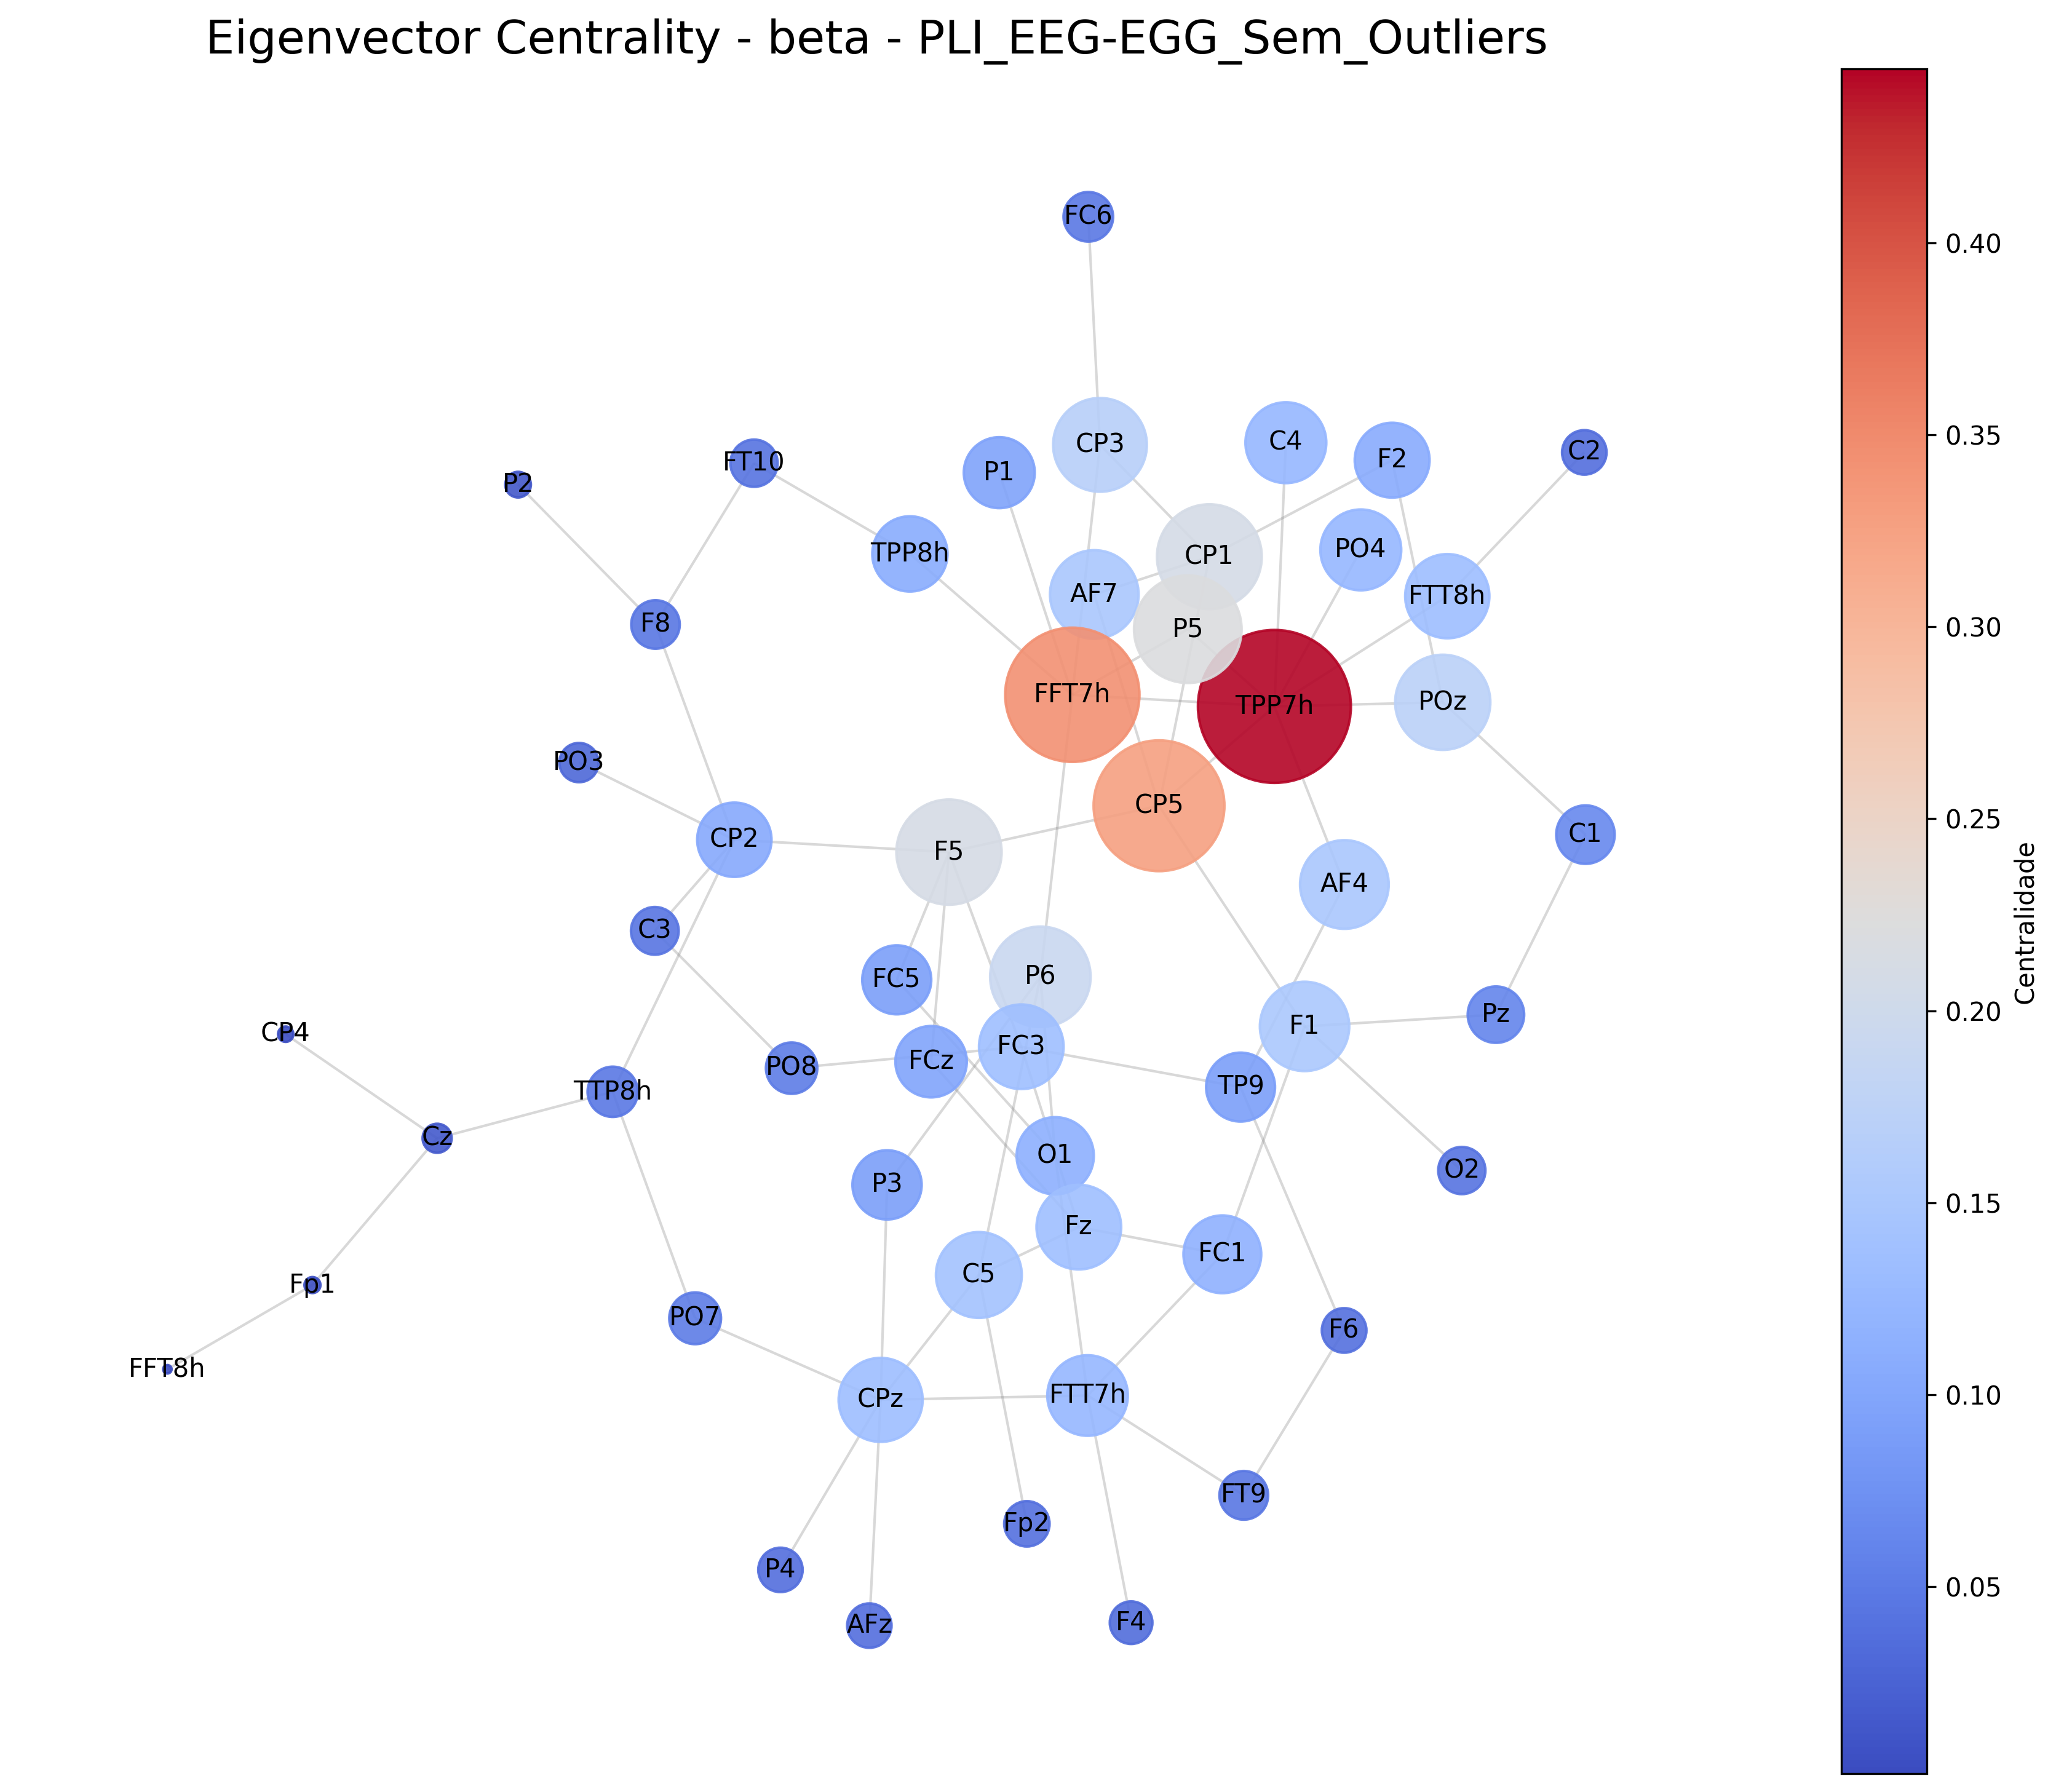
\includegraphics[width=0.45\textwidth]{figs/7_bootstrap_results_analysis/3_centrality_graphs/Sem_Outliers/Eigenvector_Centrality__beta__PLI_EEGEGG_Sem_Outliers.png}
    }
    \caption{\small \textbf{Eigenvector Centrality – Banda Beta (13--30 Hz):} A influência dos canais na rede beta muda de forma notável entre os cenários, com \textbf{TPP7h} emergindo como nodo de maior influência na versão sem outliers.}
    \label{fig:eigenvector_beta}
\end{figure}

\subsection{Banda Delta (0.5--4 Hz)}

\subsubsection{Betweenness Centrality}
\begin{figure}[H]
    \centering
    \subfloat[\small \textbf{Com Outliers:} Hierarquia – Único nodo destacado: \textbf{Fp2}.]{%
        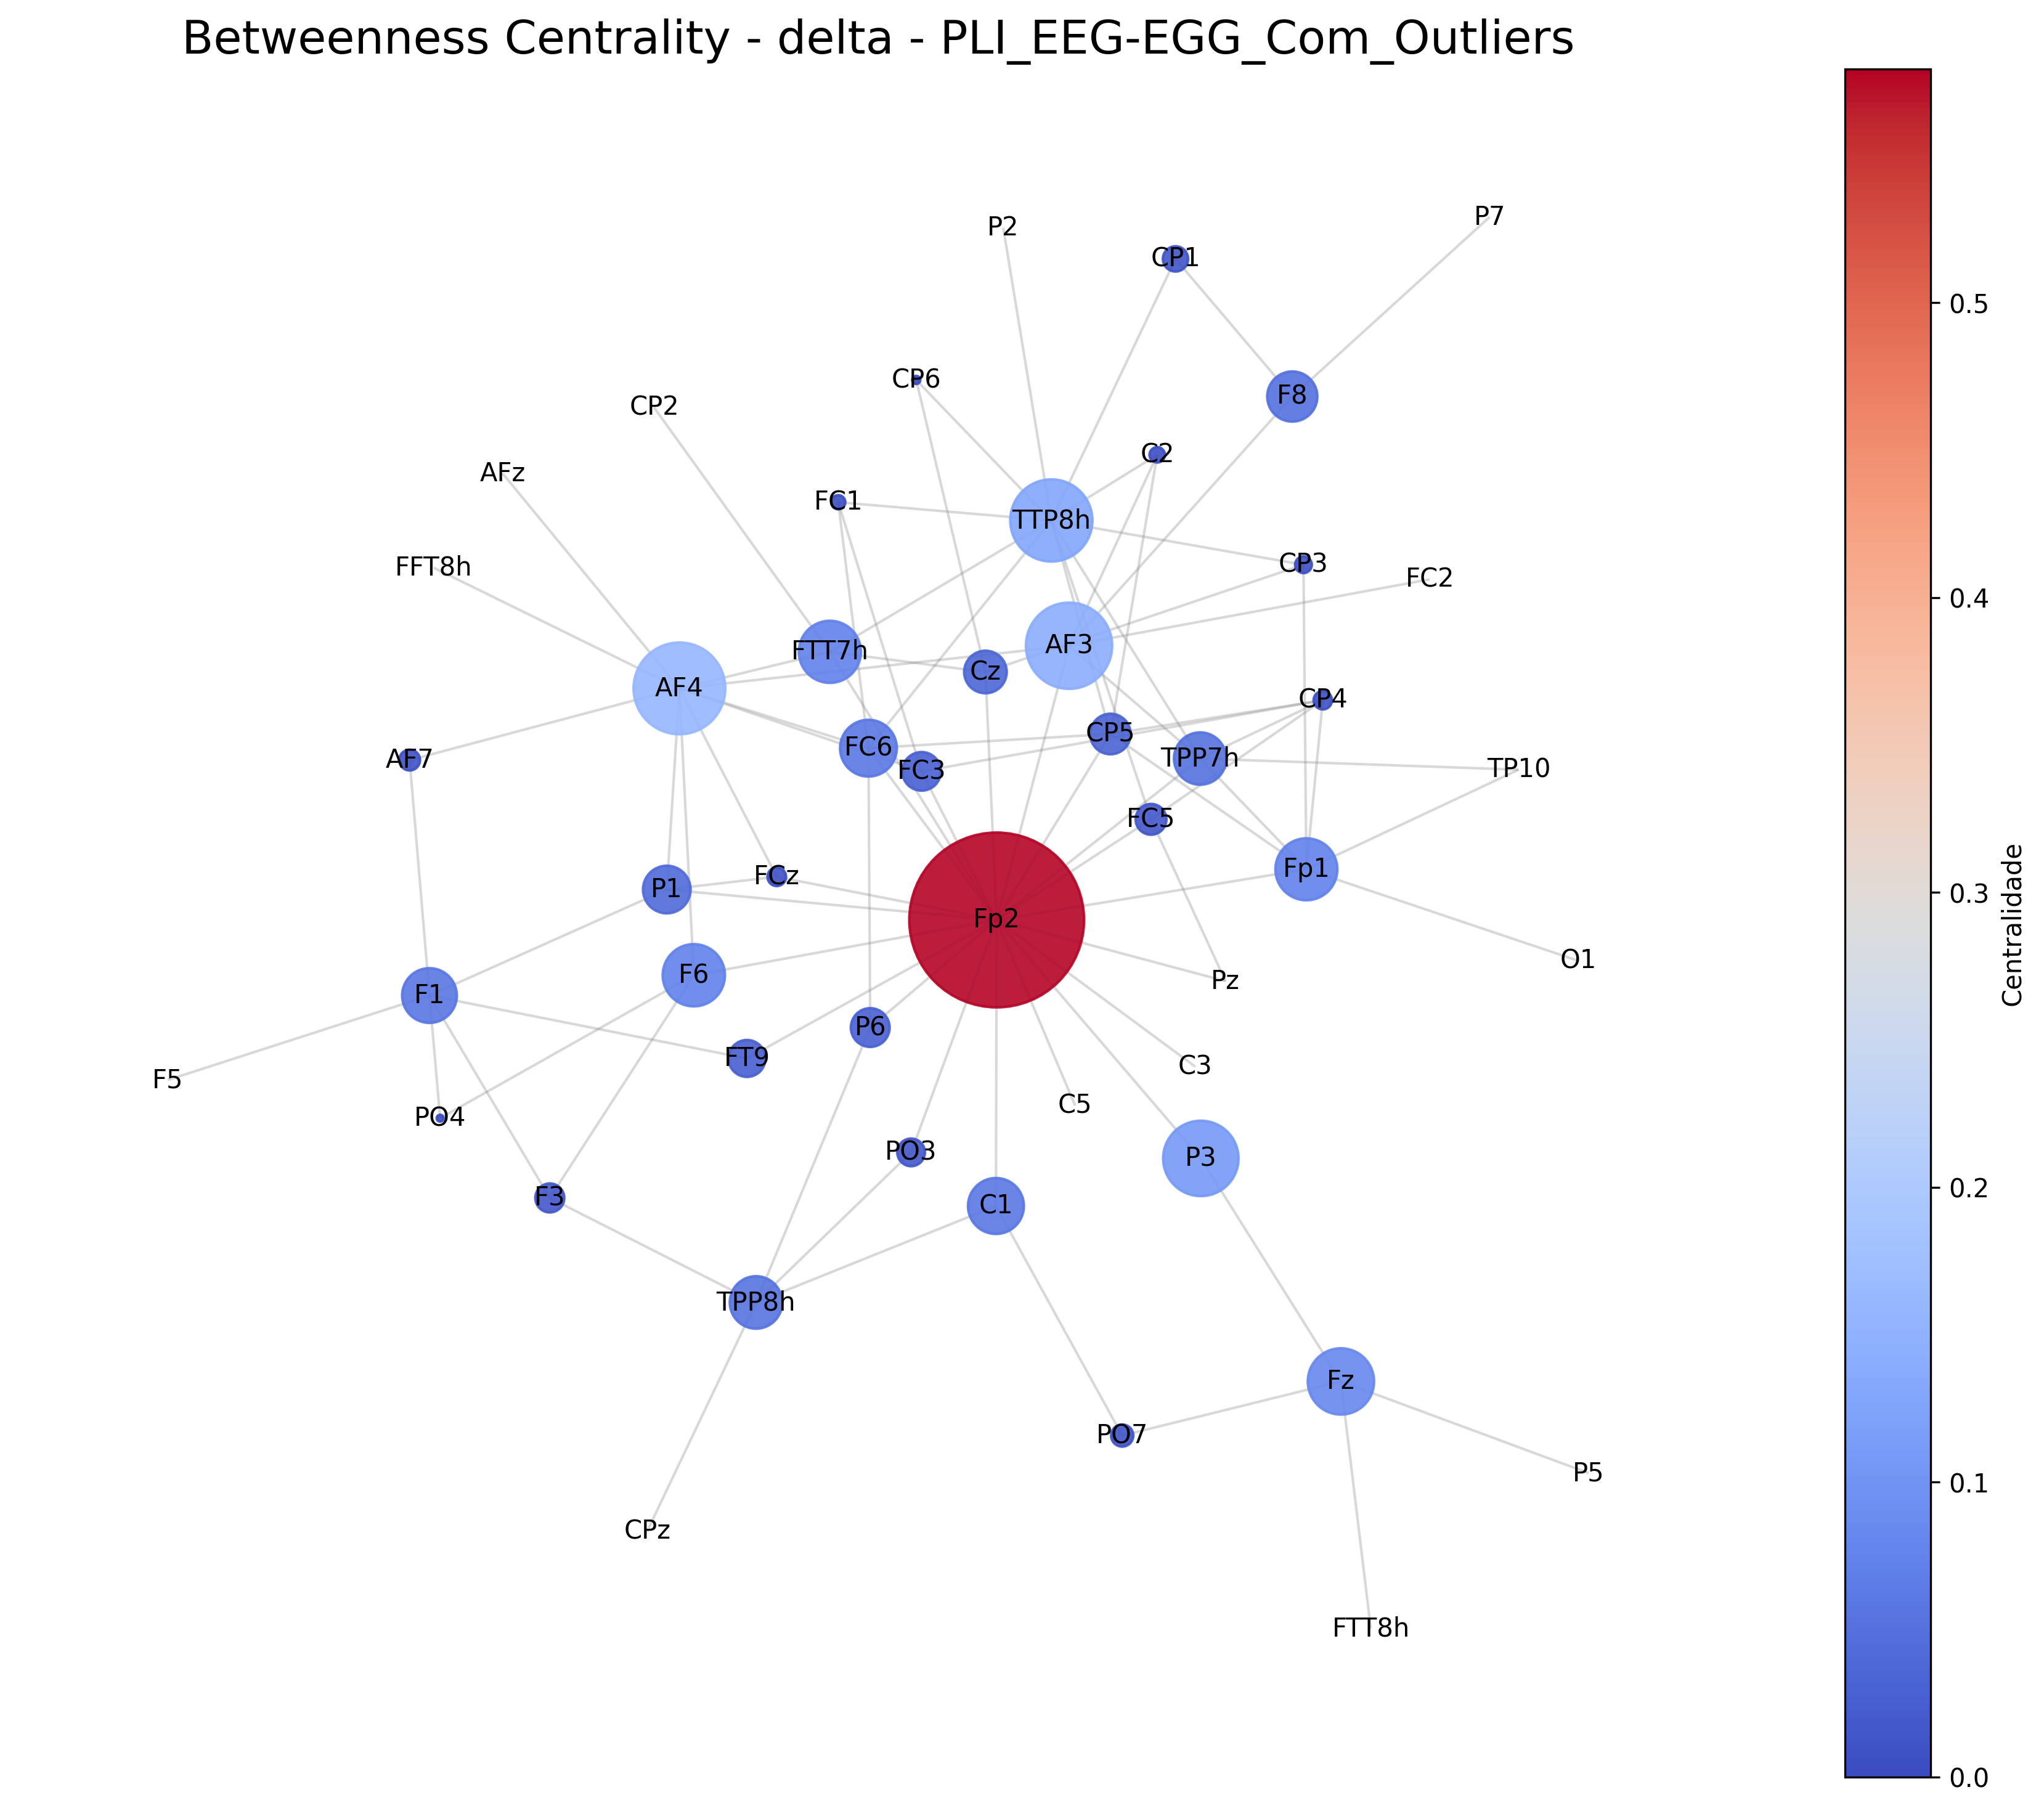
\includegraphics[width=0.45\textwidth]{figs/7_bootstrap_results_analysis/3_centrality_graphs/Com_Outliers/Betweenness_Centrality__delta__PLI_EEGEGG_Com_Outliers.png}
    }
    \hfill
    \subfloat[\small \textbf{Sem Outliers:} Hierarquia – 1. \textbf{CP5, CP4}; 2. \textbf{FC3}; 3. \textbf{AF4}; 4. \textbf{FFT8h}.]{%
        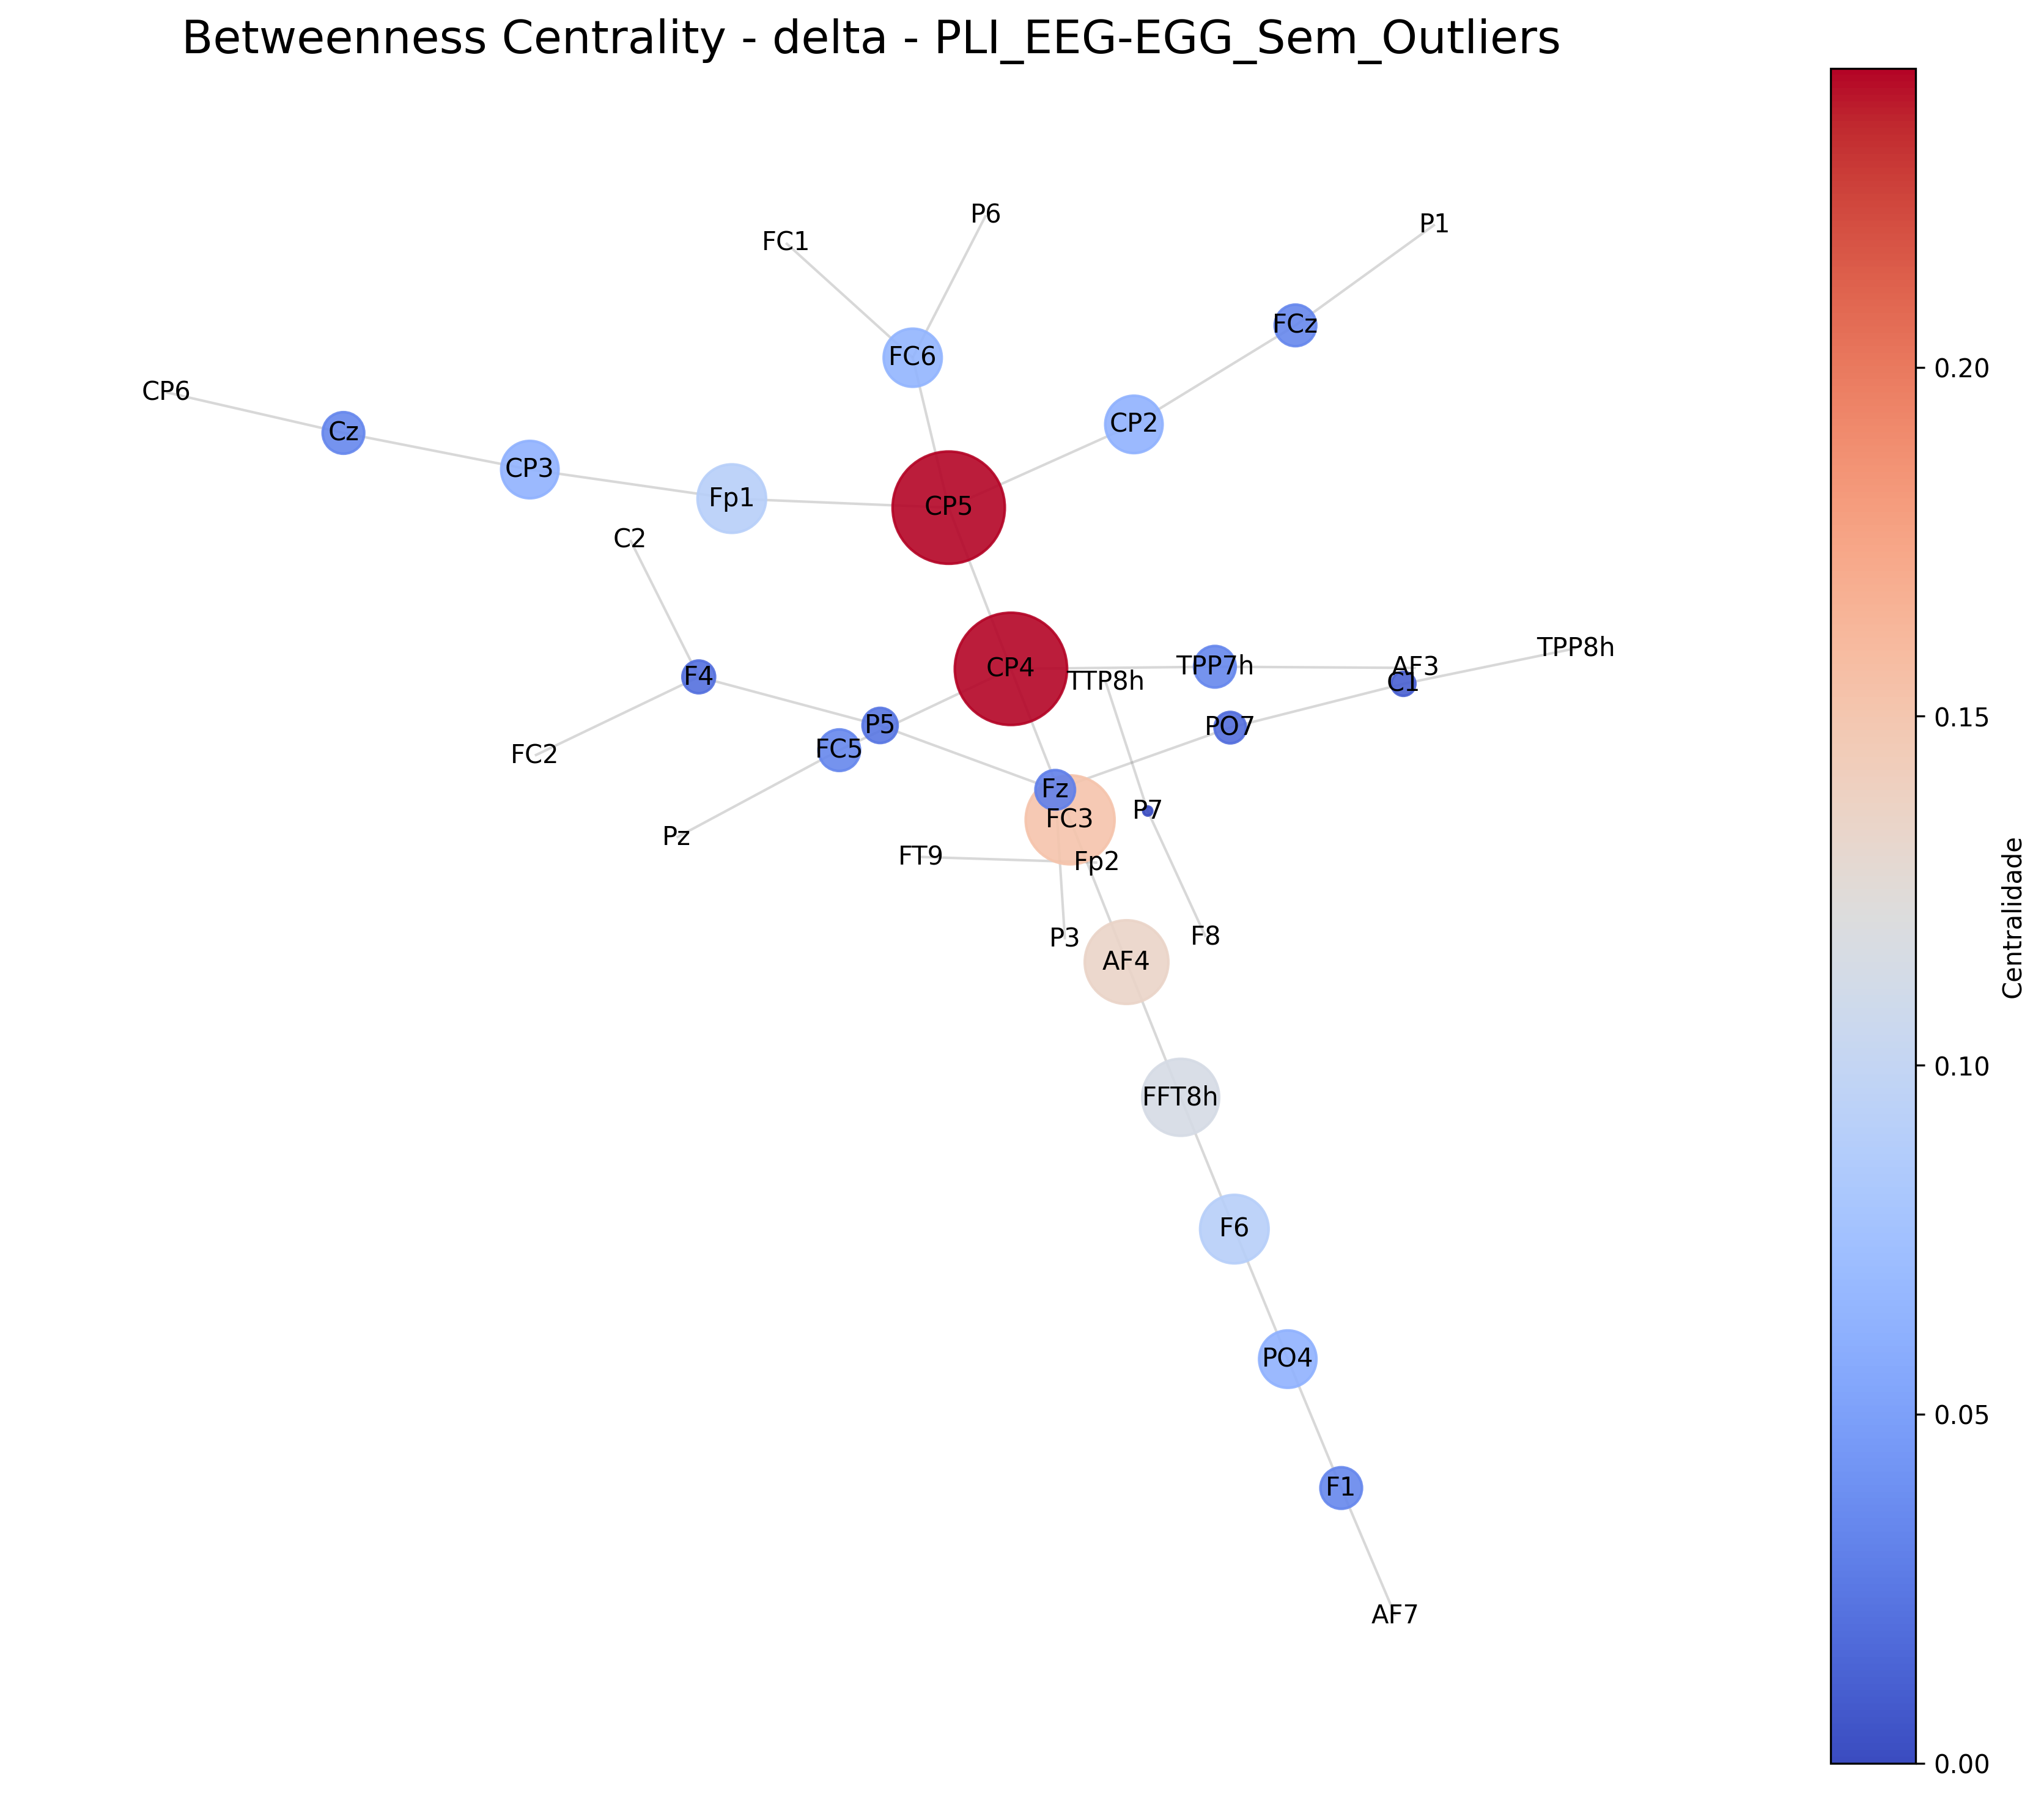
\includegraphics[width=0.45\textwidth]{figs/7_bootstrap_results_analysis/3_centrality_graphs/Sem_Outliers/Betweenness_Centrality__delta__PLI_EEGEGG_Sem_Outliers.png}
    }
    \caption{\small \textbf{Betweenness Centrality – Banda Delta (0.5--4 Hz):} A análise mostra que, com outliers, \textbf{Fp2} se destaca; sem outliers, a centralidade se redistribui com \textbf{CP5} e \textbf{CP4} assumindo papéis principais.}
    \label{fig:betweenness_delta}
\end{figure}

\subsubsection{Degree Centrality}
\begin{figure}[H]
    \centering
    \subfloat[\small \textbf{Com Outliers:} Hierarquia – 1. \textbf{Fp2}; 2. \textbf{TTP8h}; 3. \textbf{AF4}.]{%
        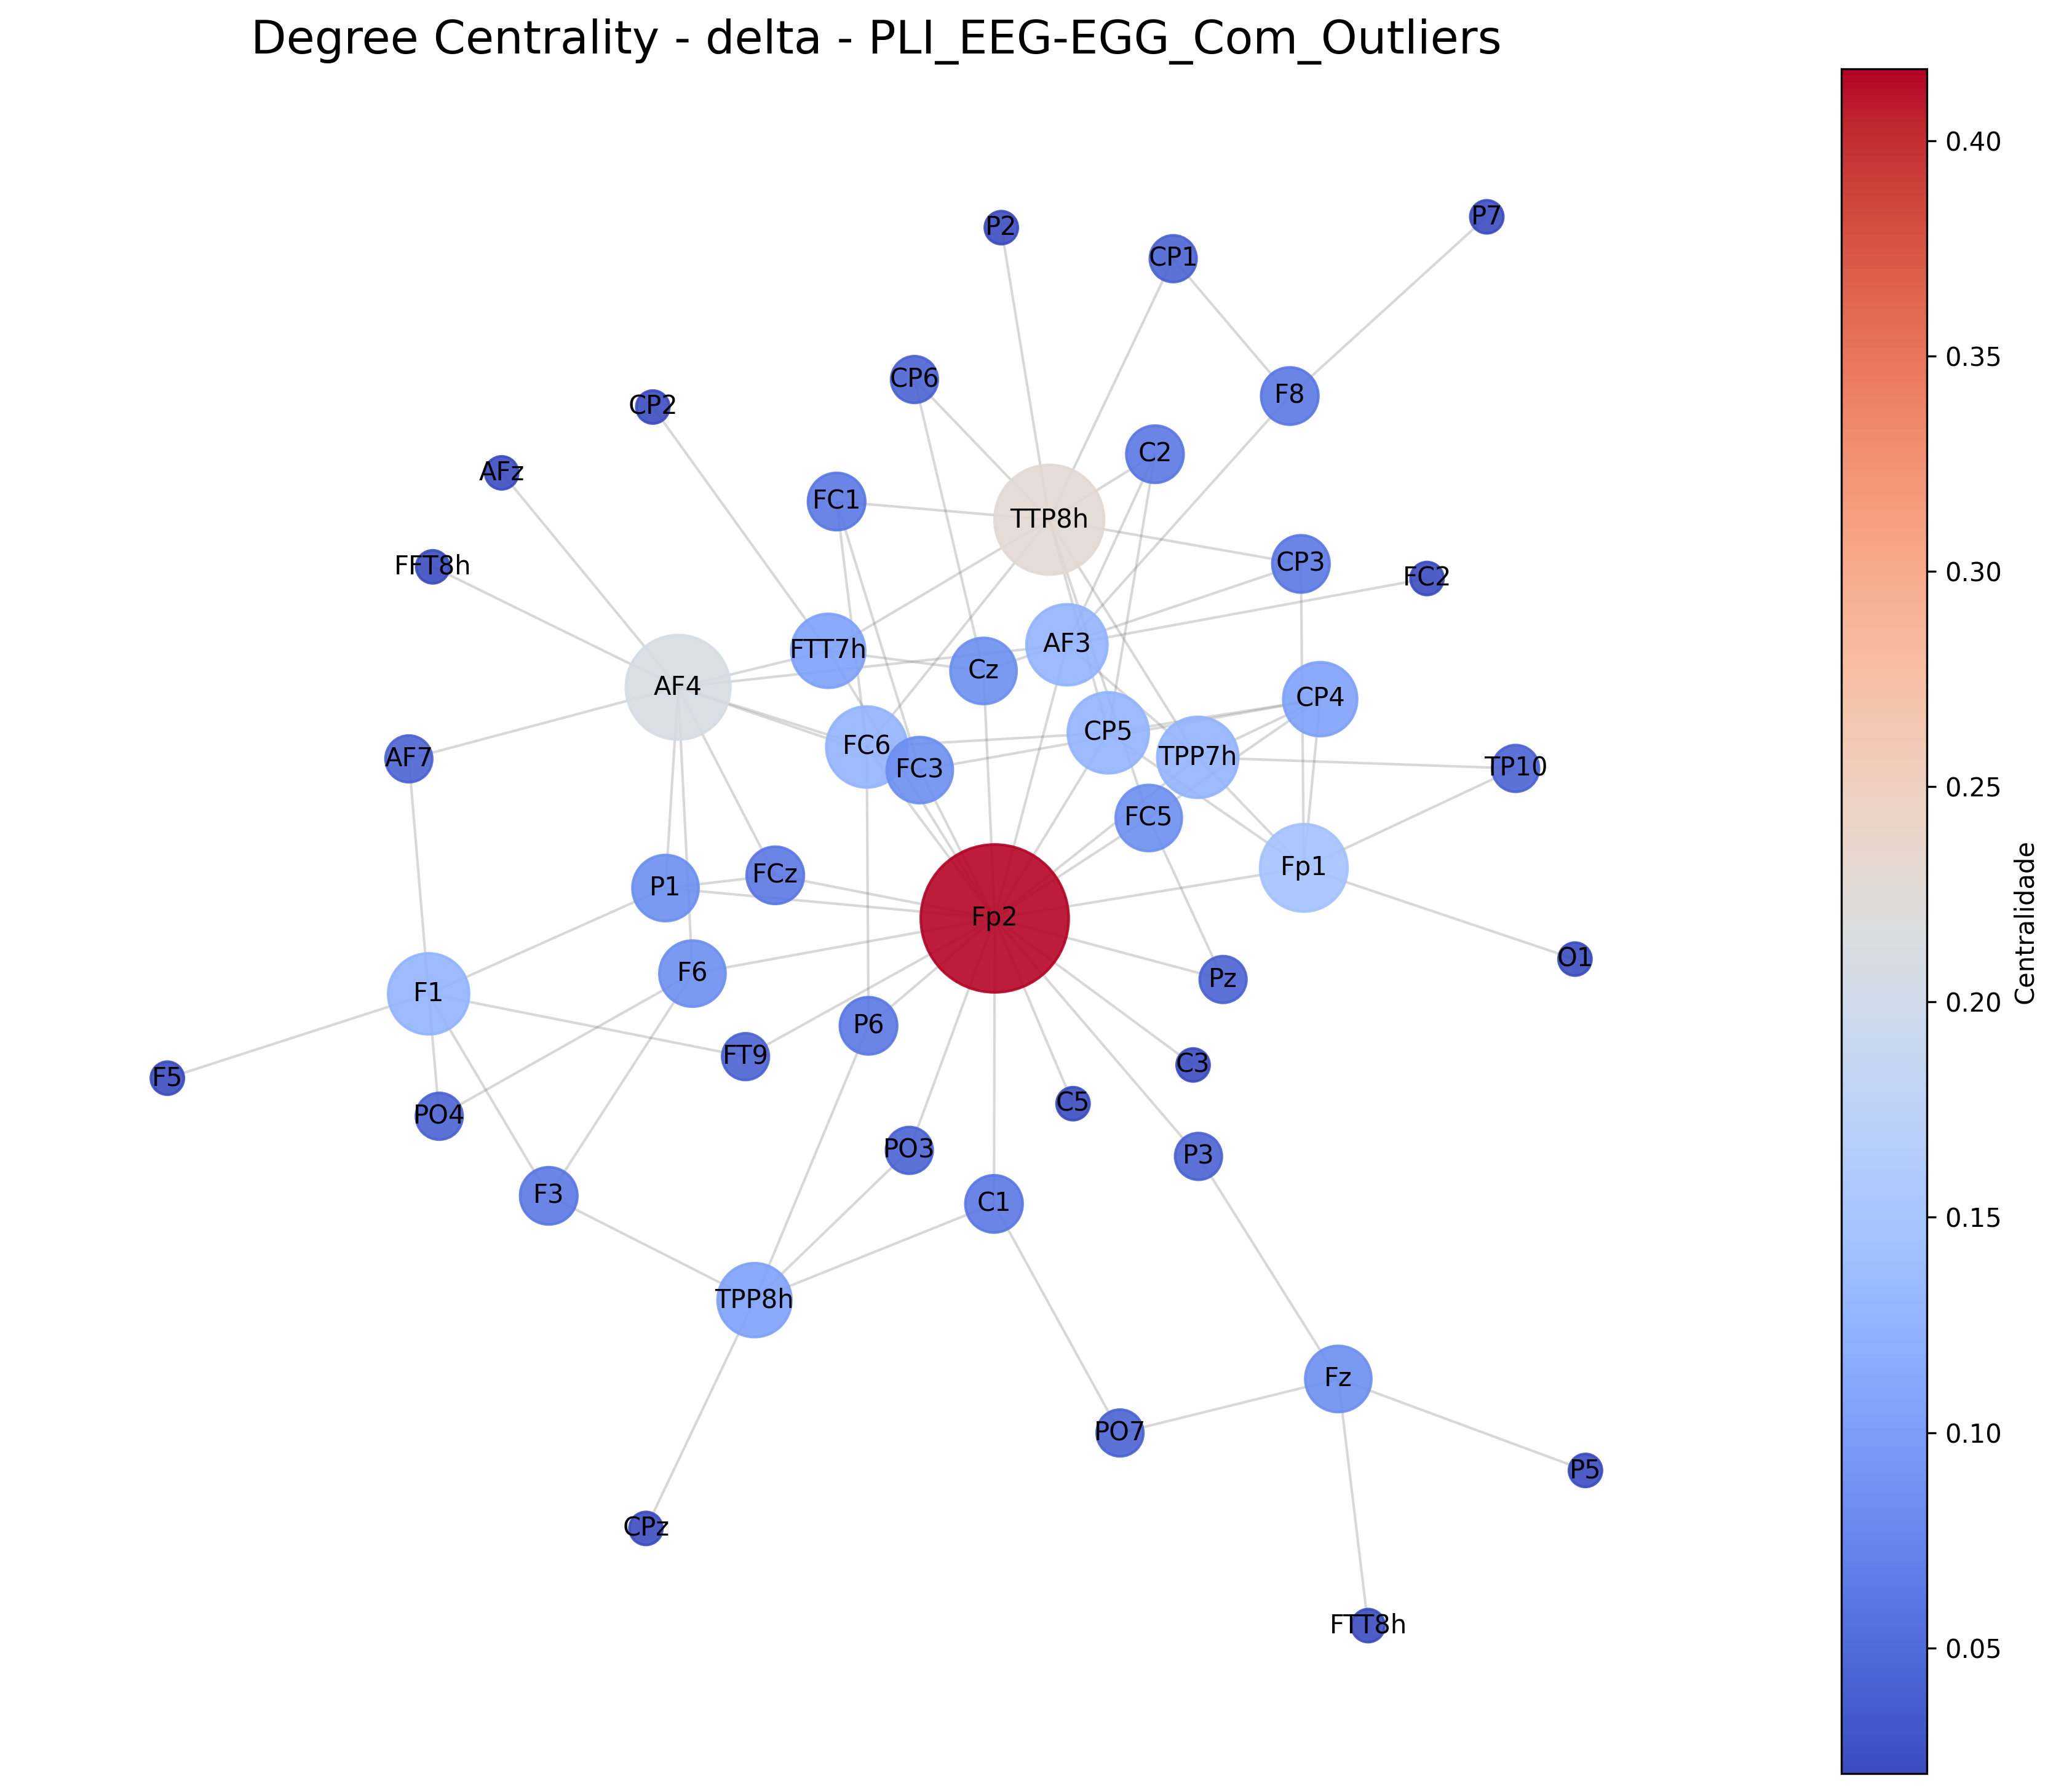
\includegraphics[width=0.45\textwidth]{figs/7_bootstrap_results_analysis/3_centrality_graphs/Com_Outliers/Degree_Centrality__delta__PLI_EEGEGG_Com_Outliers.png}
    }
    \hfill
    \subfloat[\small \textbf{Sem Outliers:} Hierarquia – 1. \textbf{CP5, CP4}; 2. \textbf{FC6, F4, Fz}.]{%
        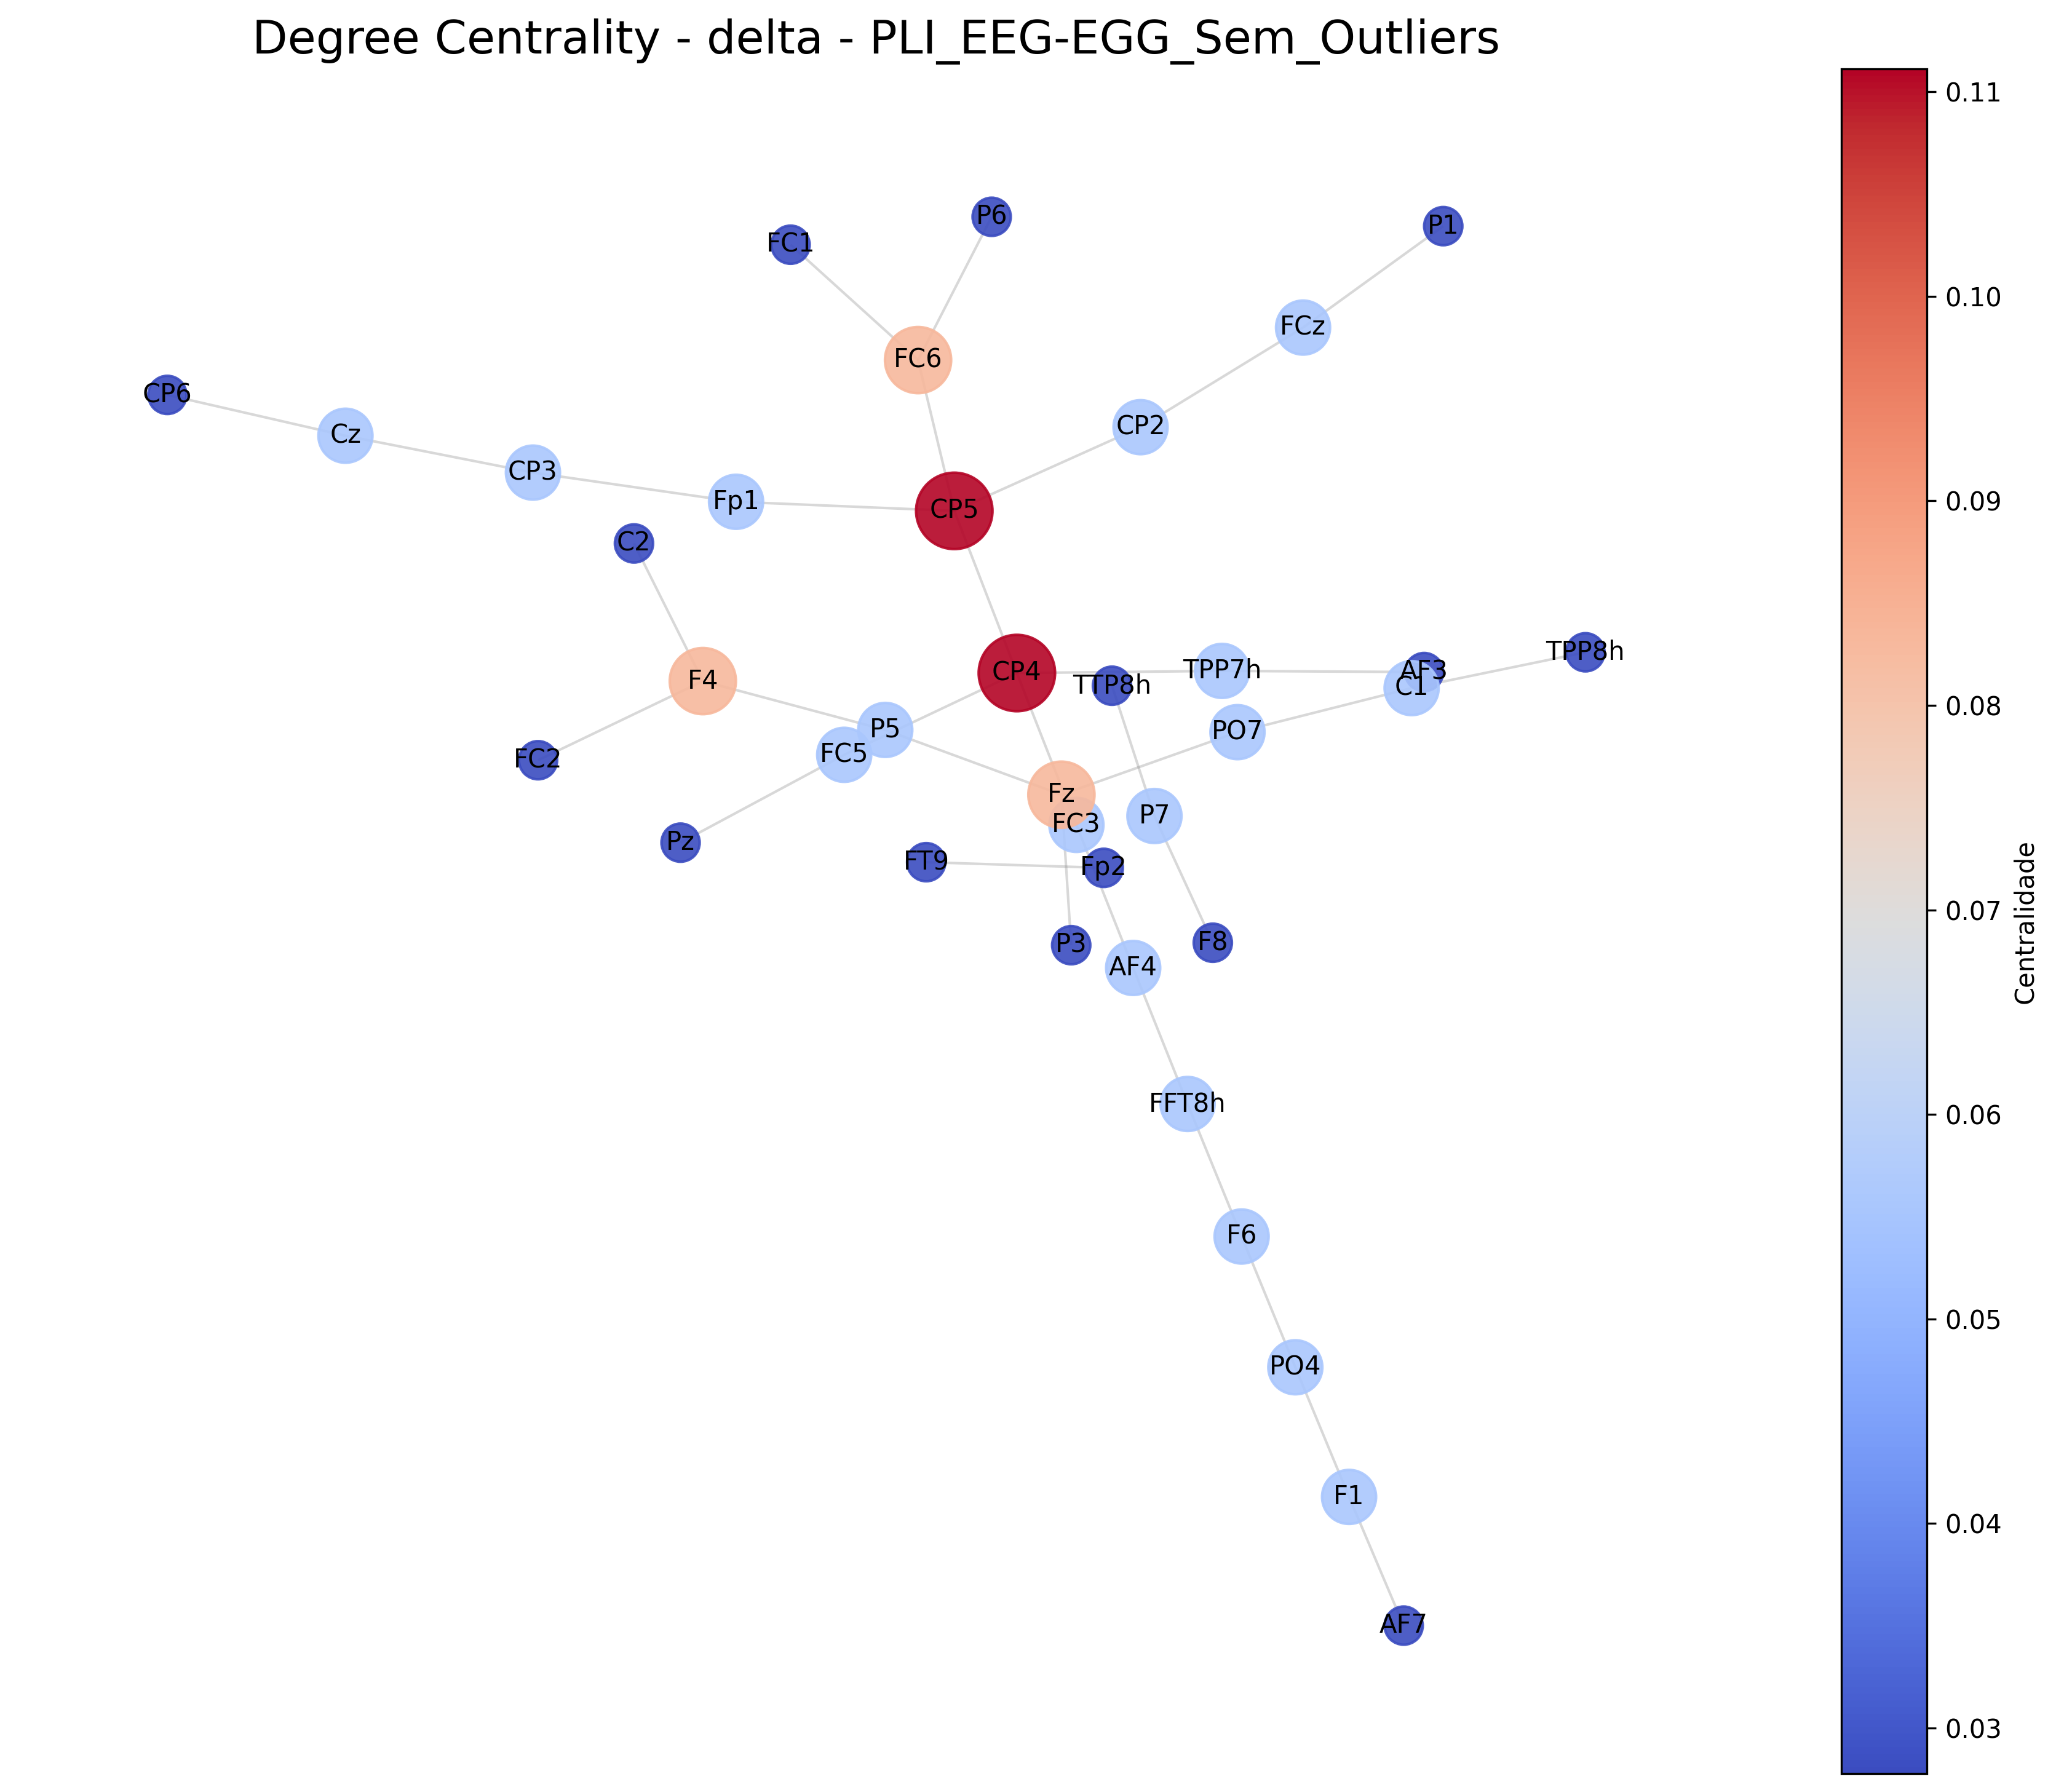
\includegraphics[width=0.45\textwidth]{figs/7_bootstrap_results_analysis/3_centrality_graphs/Sem_Outliers/Degree_Centrality__delta__PLI_EEGEGG_Sem_Outliers.png}
    }
    \caption{\small \textbf{Degree Centrality – Banda Delta (0.5--4 Hz):} A rede delta apresenta uma hierarquia distinta entre os cenários, com \textbf{Fp2} liderando na versão com outliers e um agrupamento parietal (\textbf{CP5, CP4}) emergindo sem outliers.}
    \label{fig:degree_delta}
\end{figure}

\subsubsection{Eigenvector Centrality}
\begin{figure}[H]
    \centering
    \subfloat[\small \textbf{Com Outliers:} Hierarquia – 1. \textbf{Fp2}; 2. \textbf{TTP8h, FC6, CP5, TPP7h}.]{%
        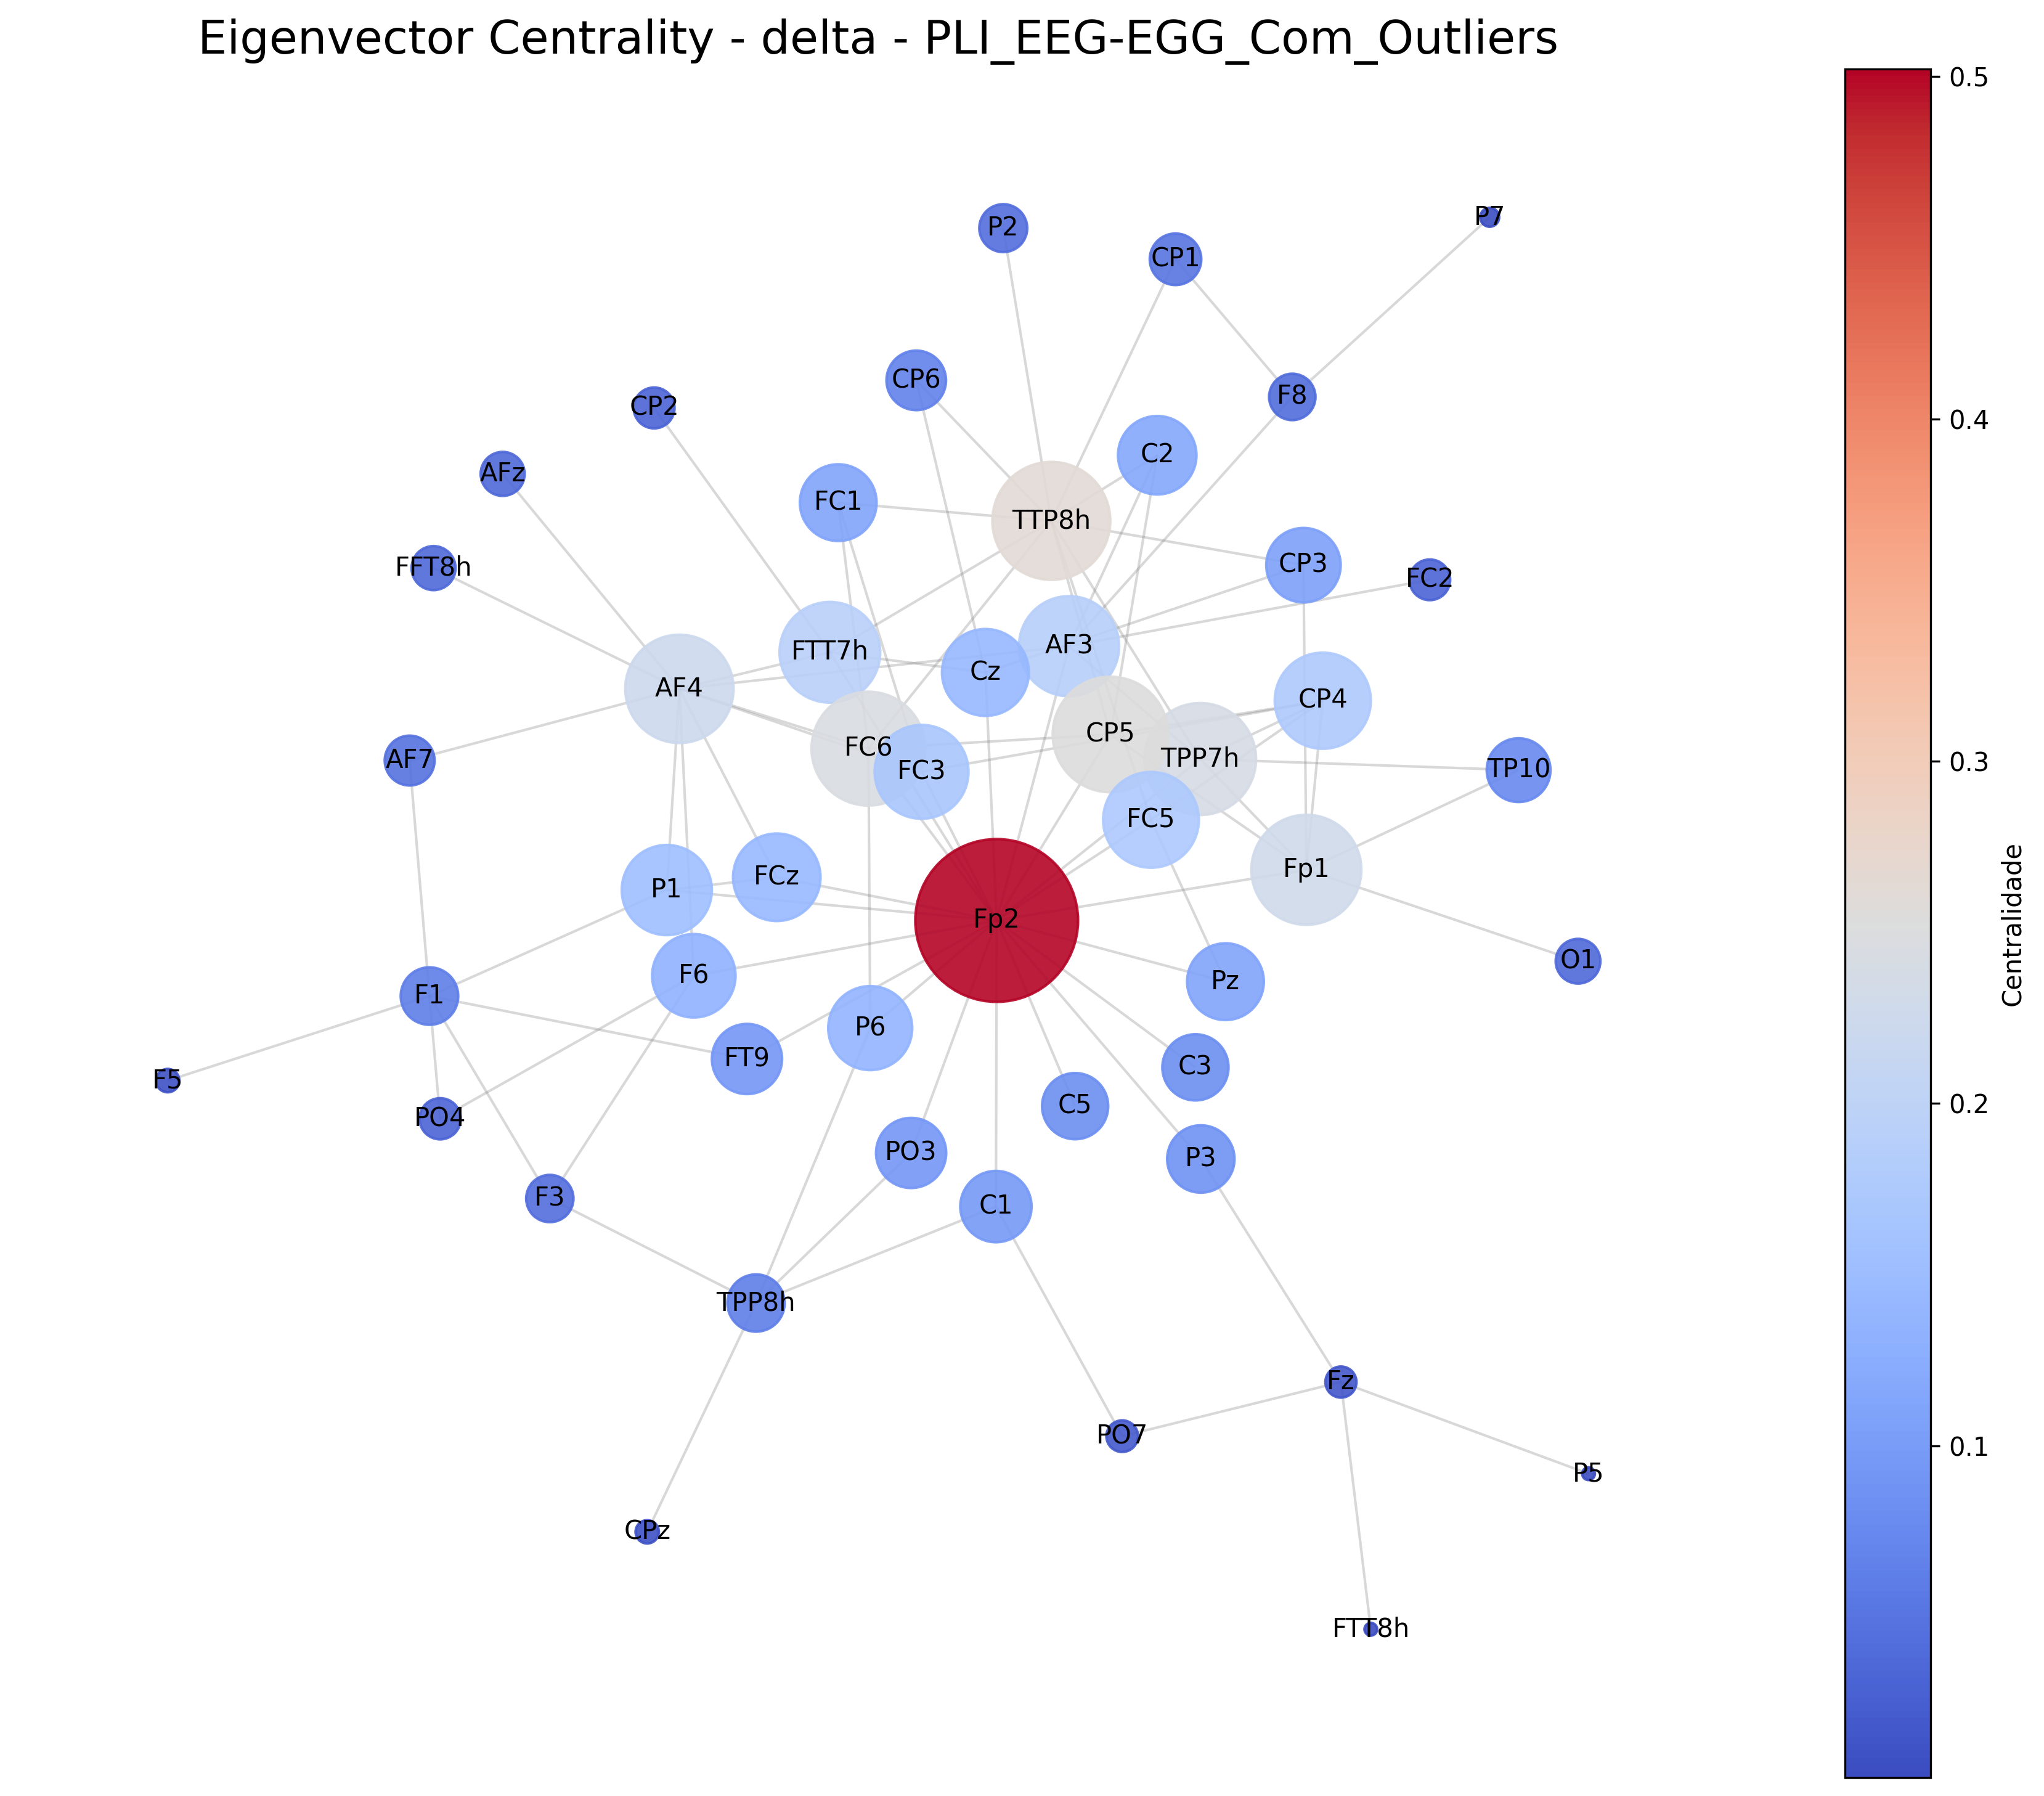
\includegraphics[width=0.45\textwidth]{figs/7_bootstrap_results_analysis/3_centrality_graphs/Com_Outliers/Eigenvector_Centrality__delta__PLI_EEGEGG_Com_Outliers.png}
    }
    \hfill
    \subfloat[\small \textbf{Sem Outliers:} Hierarquia – 1. \textbf{CP5}; 2. \textbf{CP4}; 3. \textbf{FC6}; 4. \textbf{Fp1, CP2, FC3}.]{%
        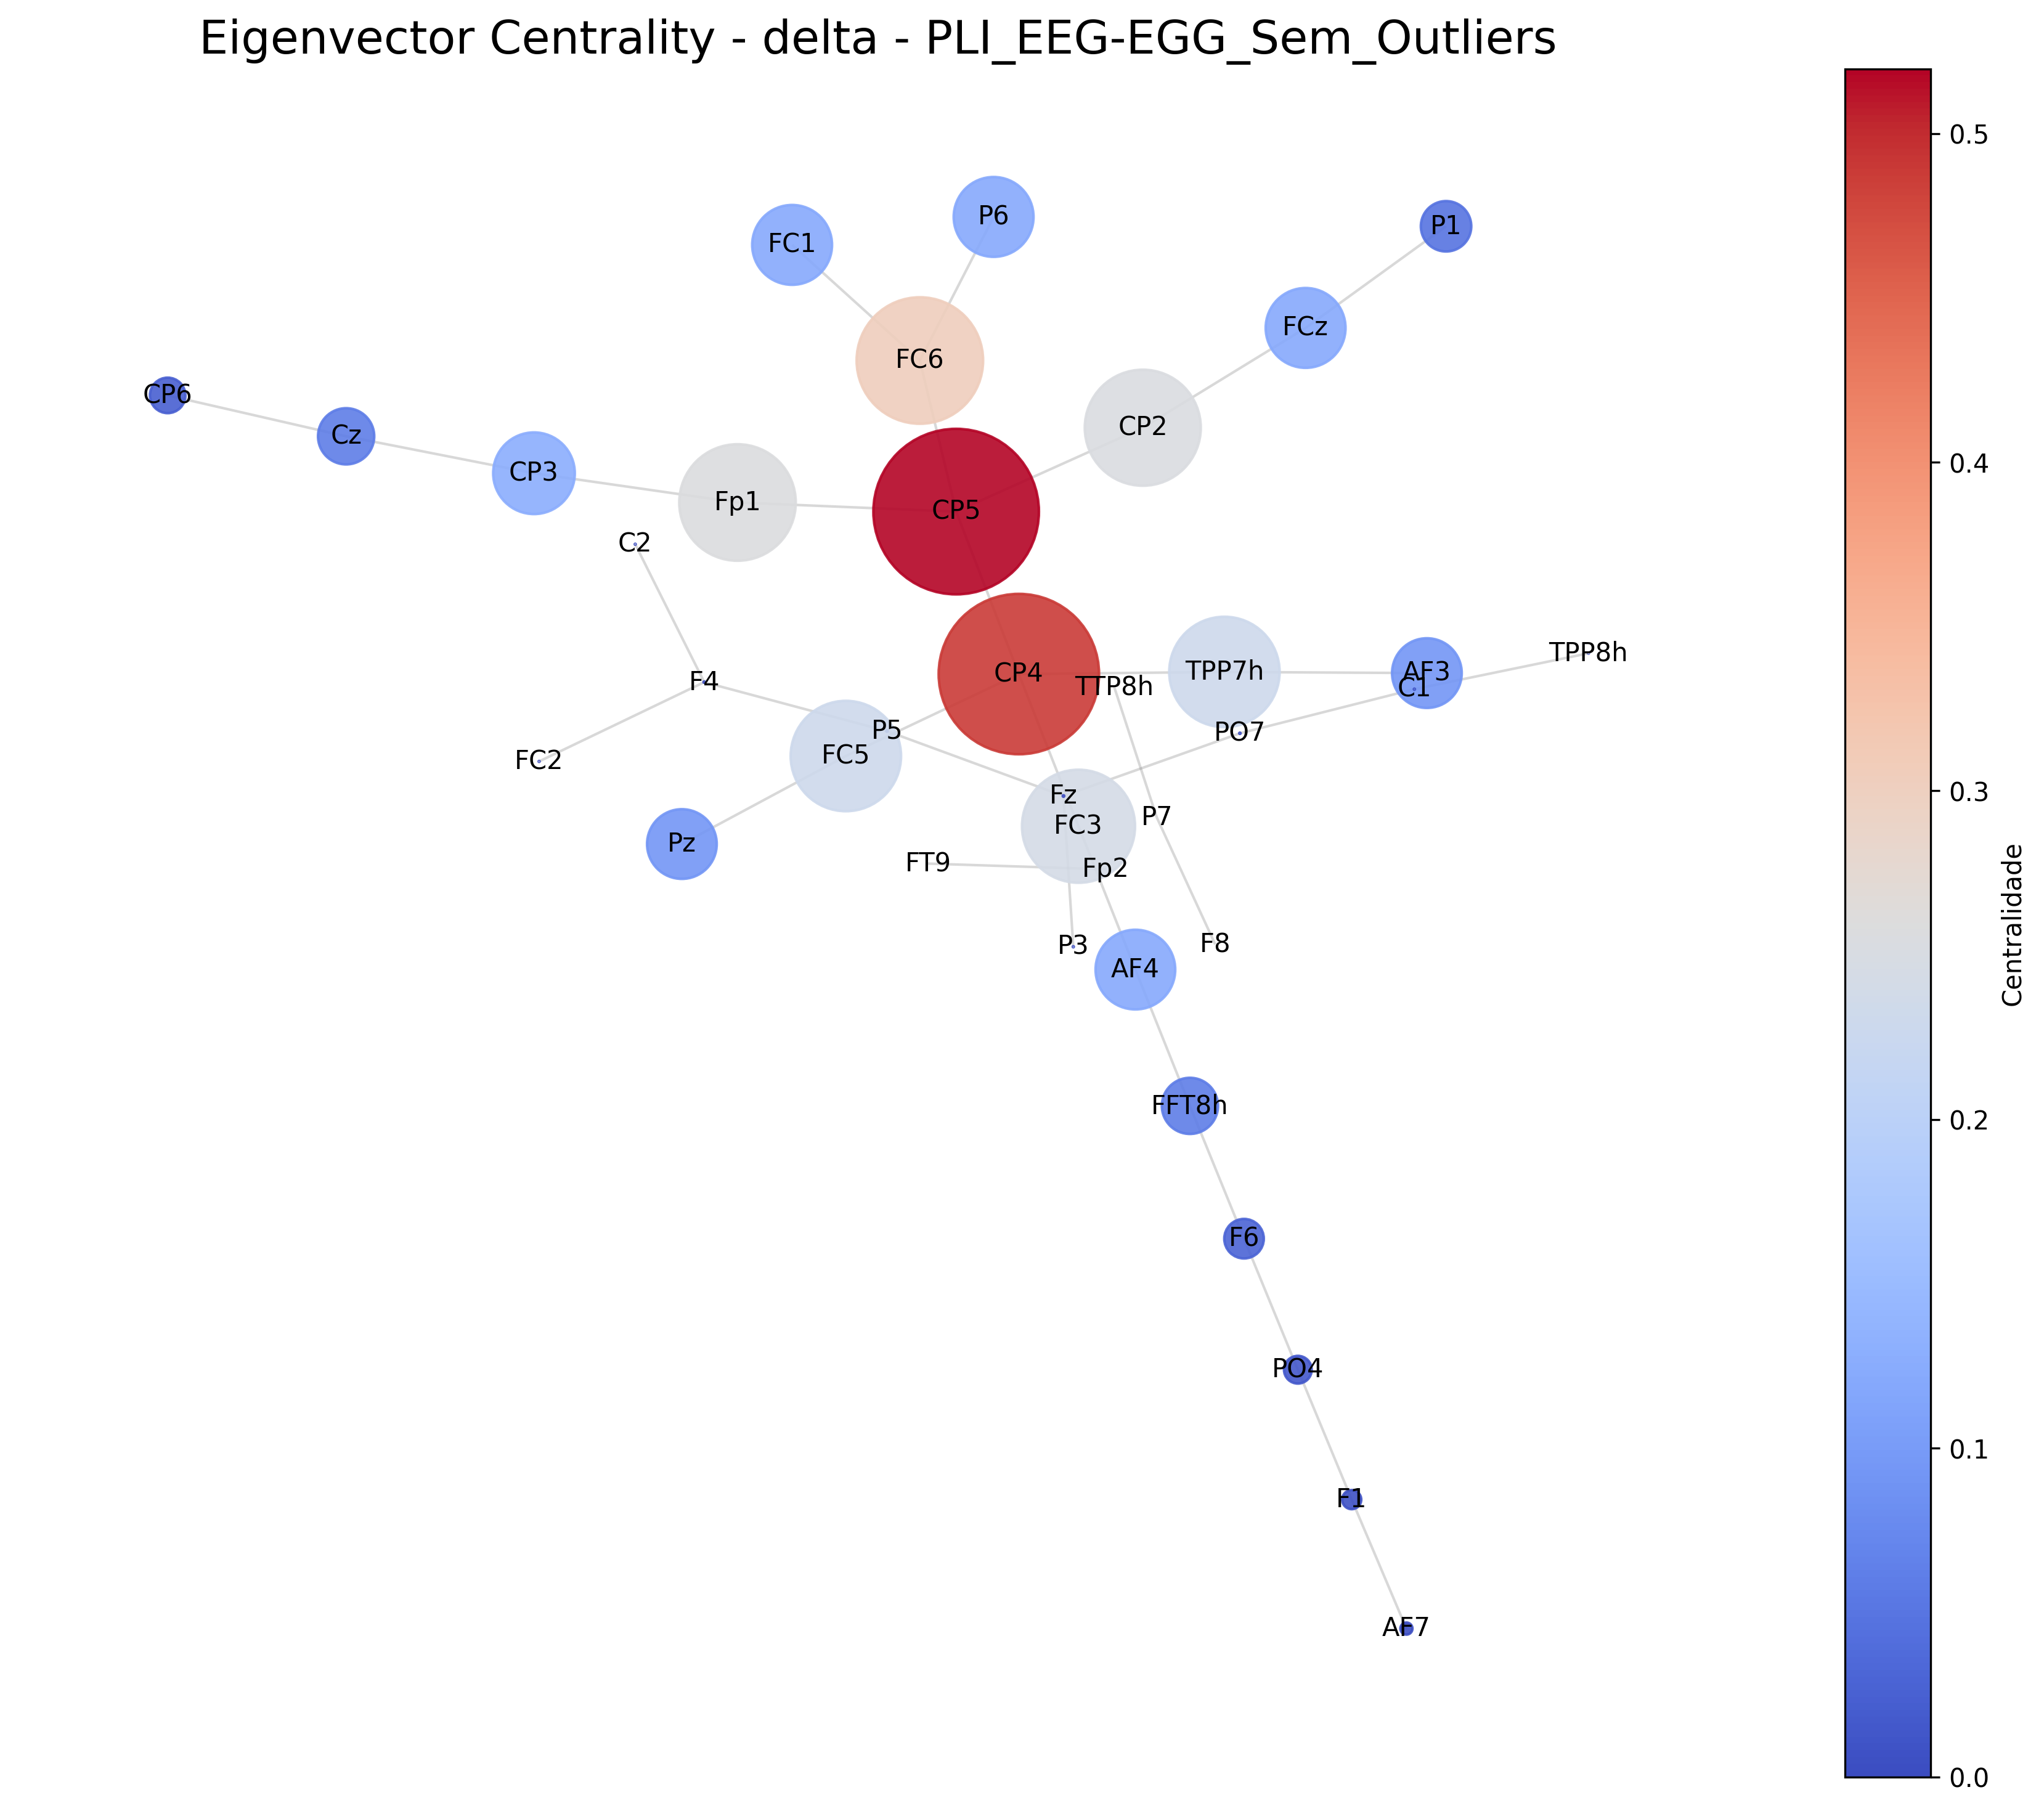
\includegraphics[width=0.45\textwidth]{figs/7_bootstrap_results_analysis/3_centrality_graphs/Sem_Outliers/Eigenvector_Centrality__delta__PLI_EEGEGG_Sem_Outliers.png}
    }
    \caption{\small \textbf{Eigenvector Centrality – Banda Delta (0.5--4 Hz):} A influência dos nodos muda após a remoção de outliers, com \textbf{CP5} emergindo como o principal na versão sem outliers.}
    \label{fig:eigenvector_delta}
\end{figure}

\subsection{Banda Gamma (30--60 Hz)}

\subsubsection{Betweenness Centrality}
\begin{figure}[H]
    \centering
    \subfloat[\small \textbf{Com Outliers:} Hierarquia – 1. \textbf{C5}; 2. \textbf{FFT8h, F3}; 3. \textbf{FT10, C1, CP4, P6}; 4. \textbf{Cz, C4, F1, Fp2, P5}.]{%
        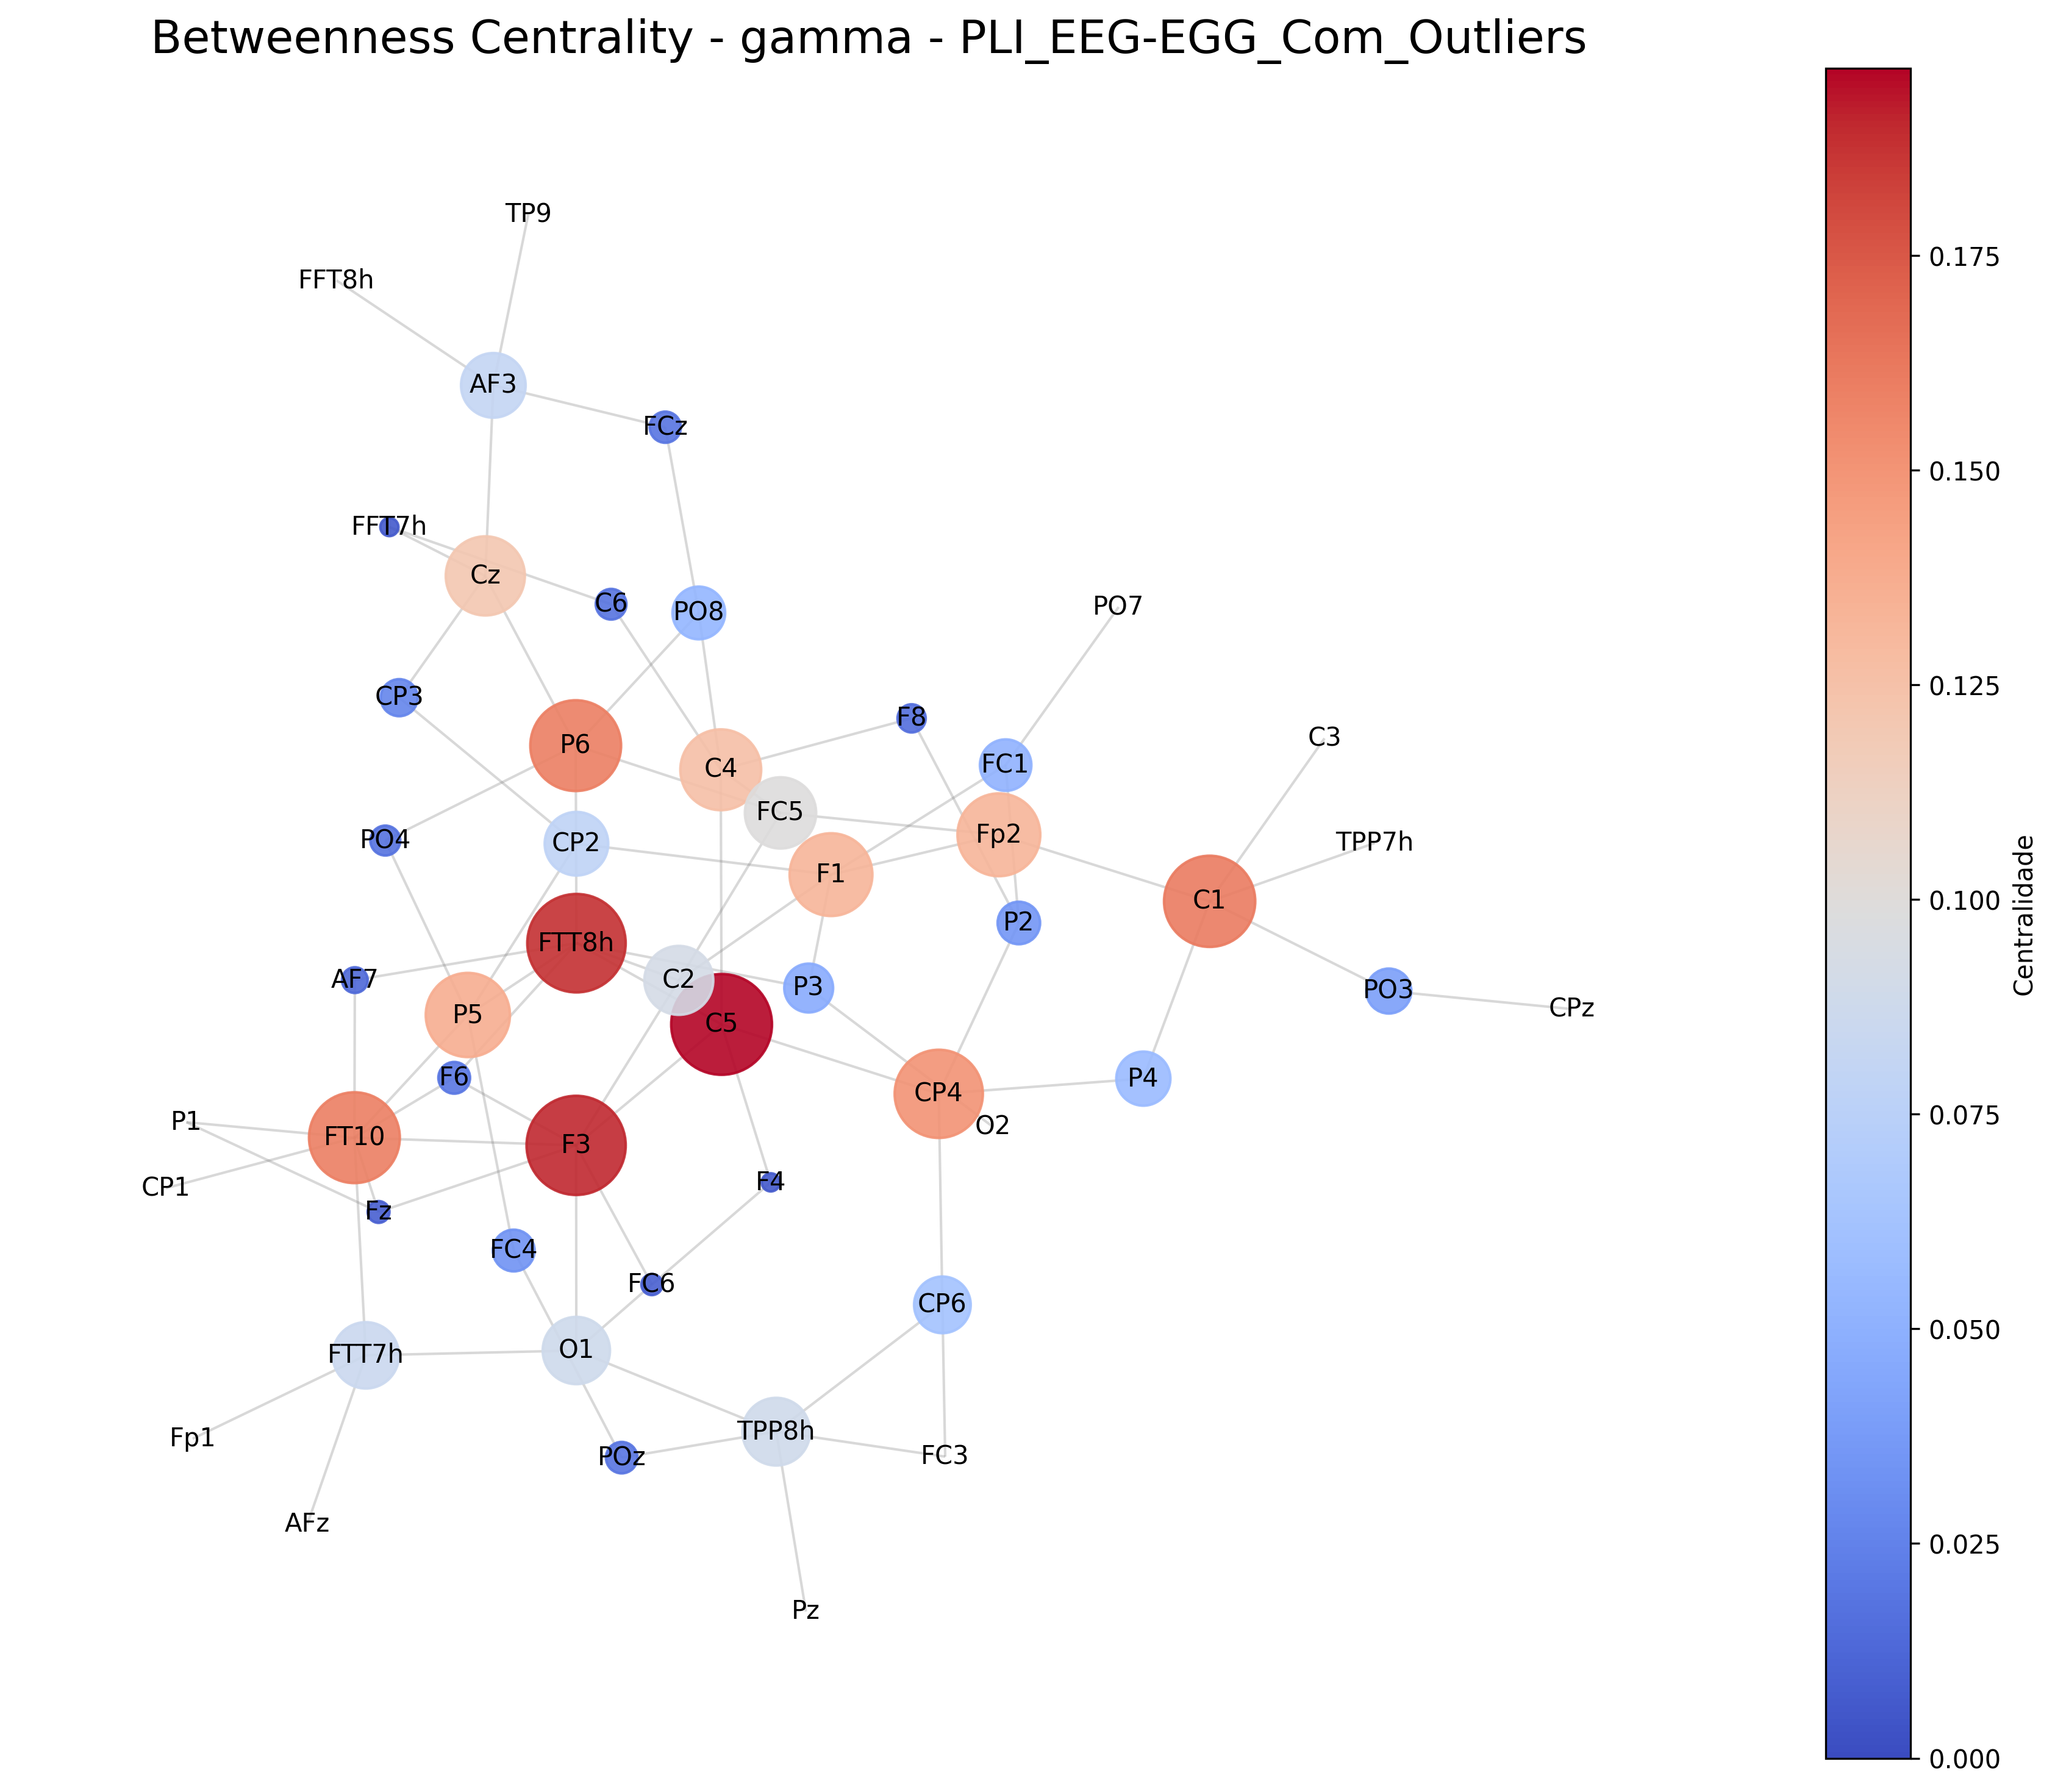
\includegraphics[width=0.45\textwidth]{figs/7_bootstrap_results_analysis/3_centrality_graphs/Com_Outliers/Betweenness_Centrality__gamma__PLI_EEGEGG_Com_Outliers.png}
    }
    \hfill
    \subfloat[\small \textbf{Sem Outliers:} Hierarquia – 1. \textbf{F3}; 2. \textbf{C5}; 3. \textbf{FFT8h, FT10}; 4. \textbf{P5}.]{%
        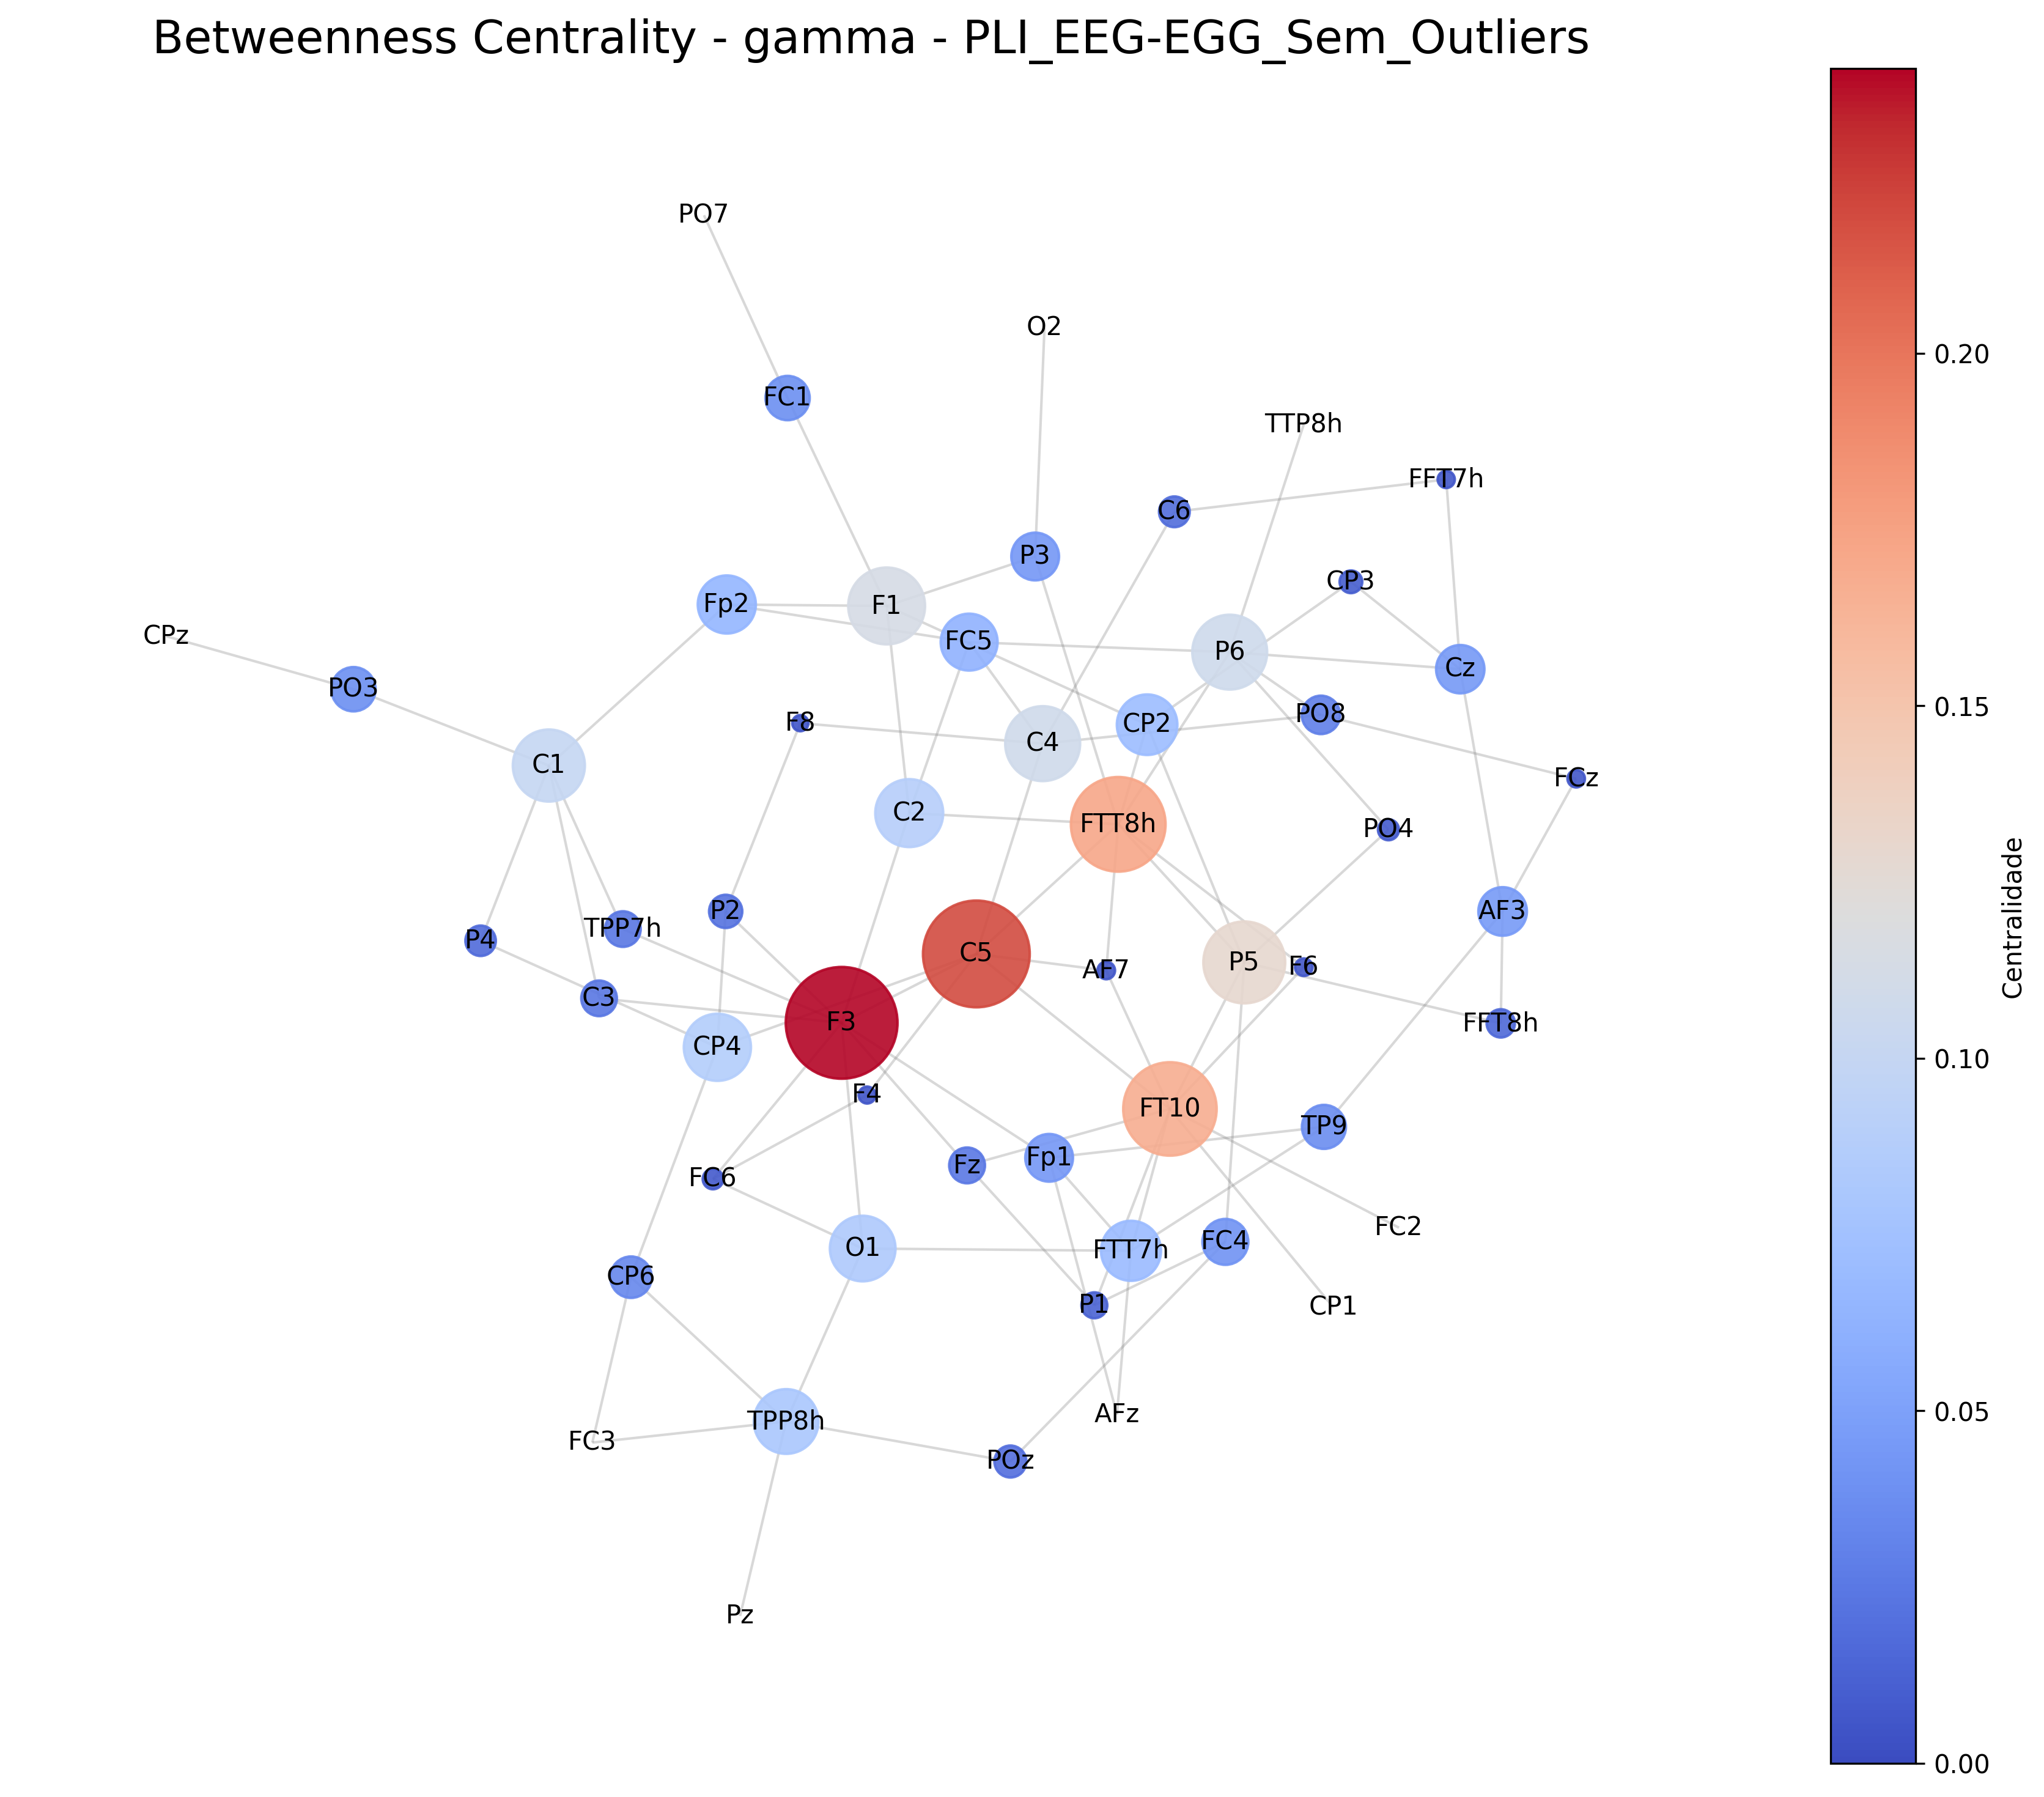
\includegraphics[width=0.45\textwidth]{figs/7_bootstrap_results_analysis/3_centrality_graphs/Sem_Outliers/Betweenness_Centrality__gamma__PLI_EEGEGG_Sem_Outliers.png}
    }
    \caption{\small \textbf{Betweenness Centrality – Banda Gamma (30--60 Hz):} A hierarquia dos canais na rede gamma apresenta uma divisão mais complexa, com uma diminuição geral dos valores na versão sem outliers.}
    \label{fig:betweenness_gamma}
\end{figure}

\subsubsection{Degree Centrality}
\begin{figure}[H]
    \centering
    \subfloat[\small \textbf{Com Outliers:} Hierarquia – 1. \textbf{FT10}; 2. \textbf{FTT8h}; 3. \textbf{F3}; 4. \textbf{P5, P6, C4, F1, C5, C1, TPP8h}.]{%
        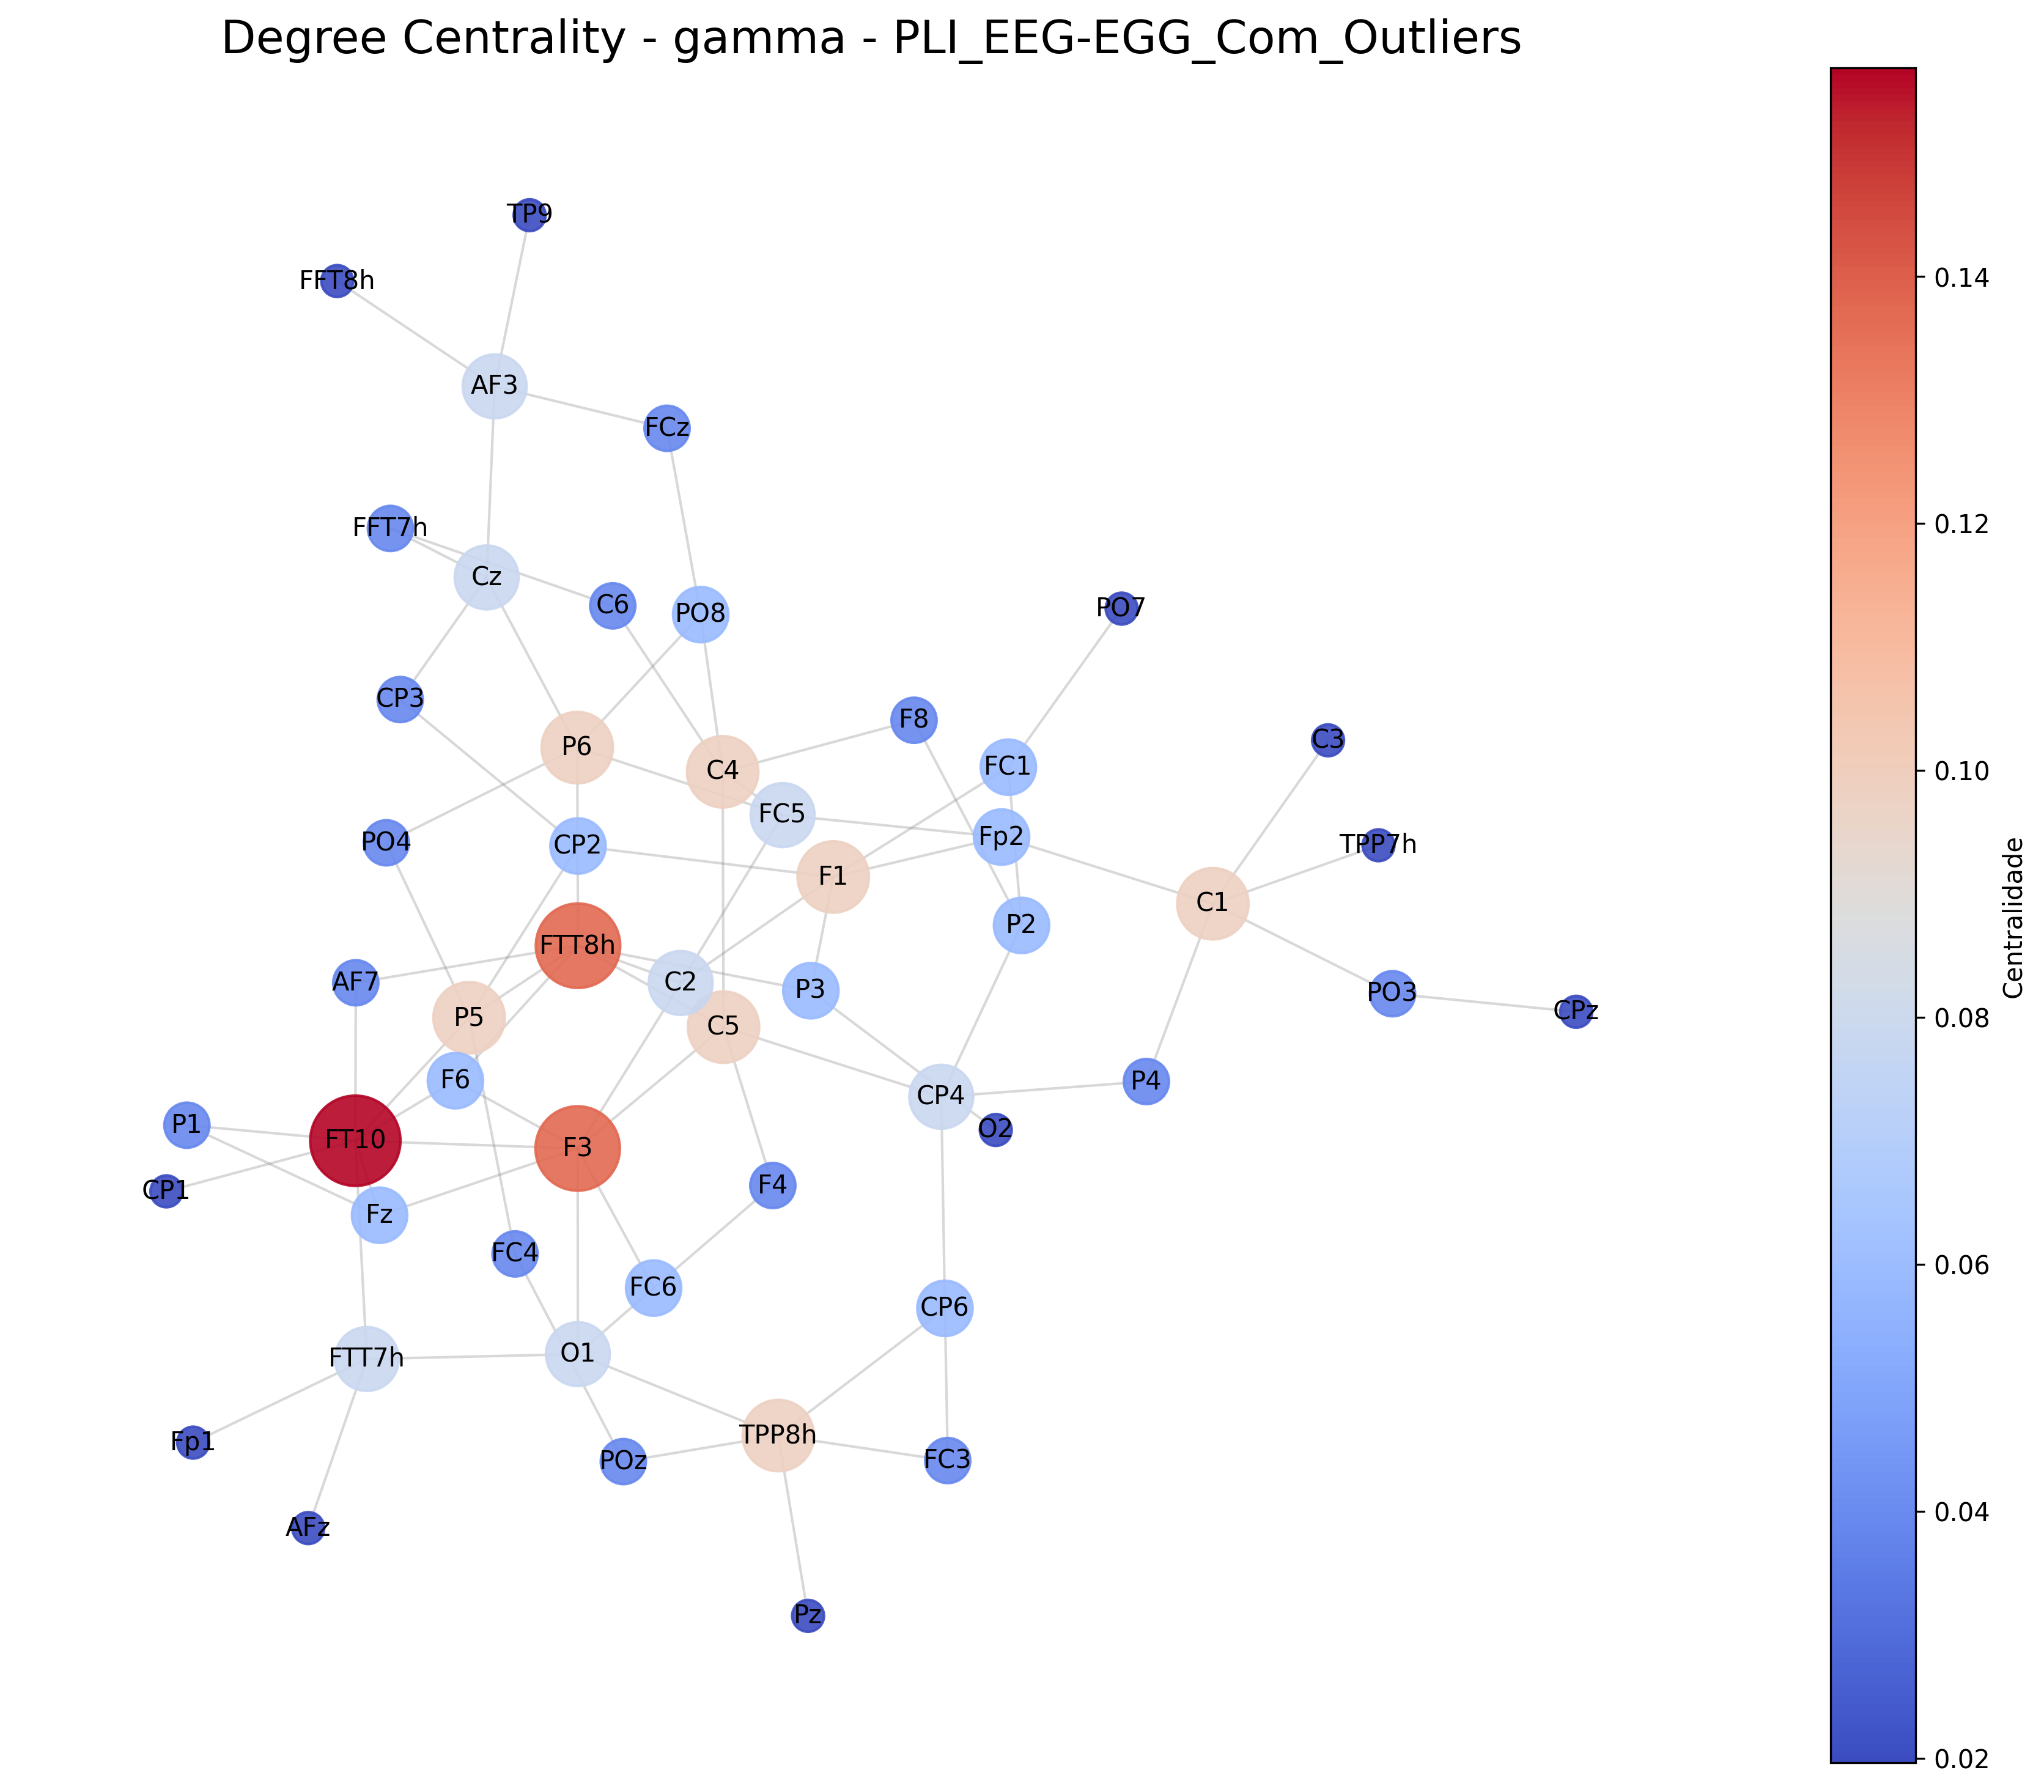
\includegraphics[width=0.45\textwidth]{figs/7_bootstrap_results_analysis/3_centrality_graphs/Com_Outliers/Degree_Centrality__gamma__PLI_EEGEGG_Com_Outliers.png}
    }
    \hfill
    \subfloat[\small \textbf{Sem Outliers:} Hierarquia – 1. \textbf{F3, FT10}; 2. \textbf{FTT8h}; 3. \textbf{C5}; 4. \textbf{P5, P6}.]{%
        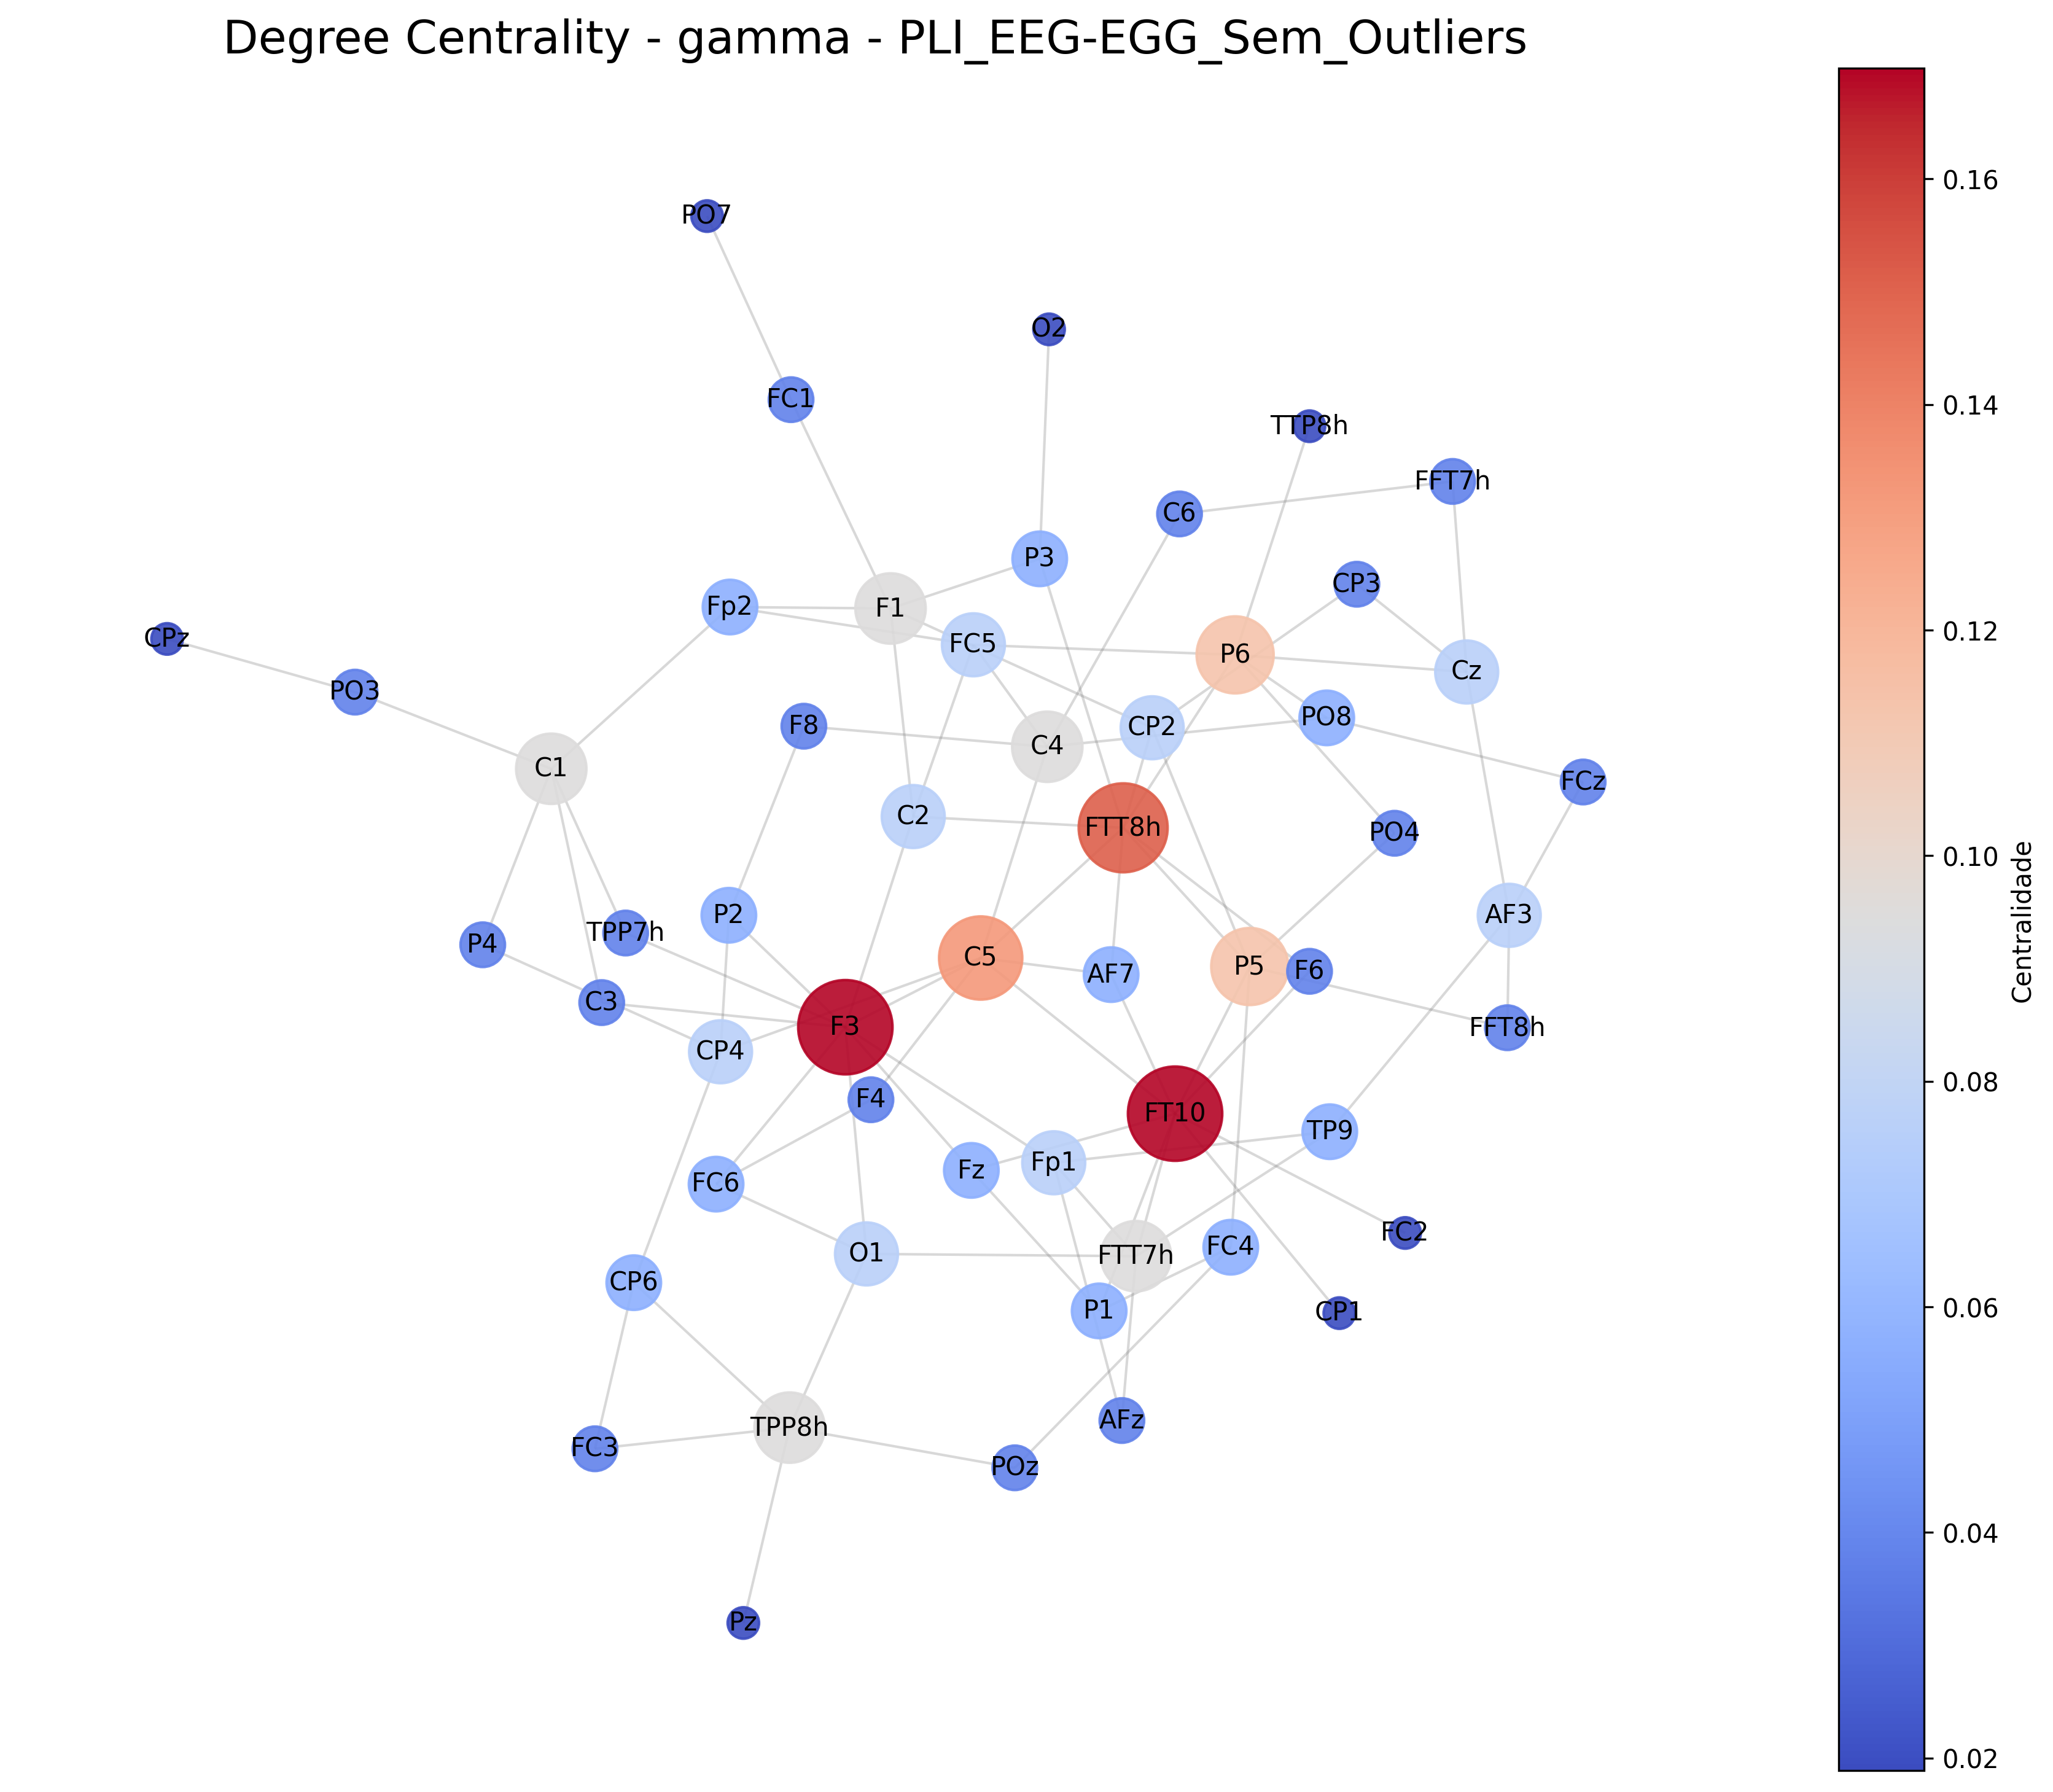
\includegraphics[width=0.45\textwidth]{figs/7_bootstrap_results_analysis/3_centrality_graphs/Sem_Outliers/Degree_Centrality__gamma__PLI_EEGEGG_Sem_Outliers.png}
    }
    \caption{\small \textbf{Degree Centrality – Banda Gamma (30--60 Hz):} Os canais de maior conectividade direta mudam levemente entre os cenários, com uma hierarquia consistente na versão sem outliers.}
    \label{fig:degree_gamma}
\end{figure}

\subsubsection{Eigenvector Centrality}
\begin{figure}[H]
    \centering
    \subfloat[\small \textbf{Com Outliers:} Hierarquia – 1. \textbf{F3, FT10}; 2. \textbf{FTT8h}; 3. \textbf{F6}; 4. \textbf{Fz, P5, C2, C5}.]{%
        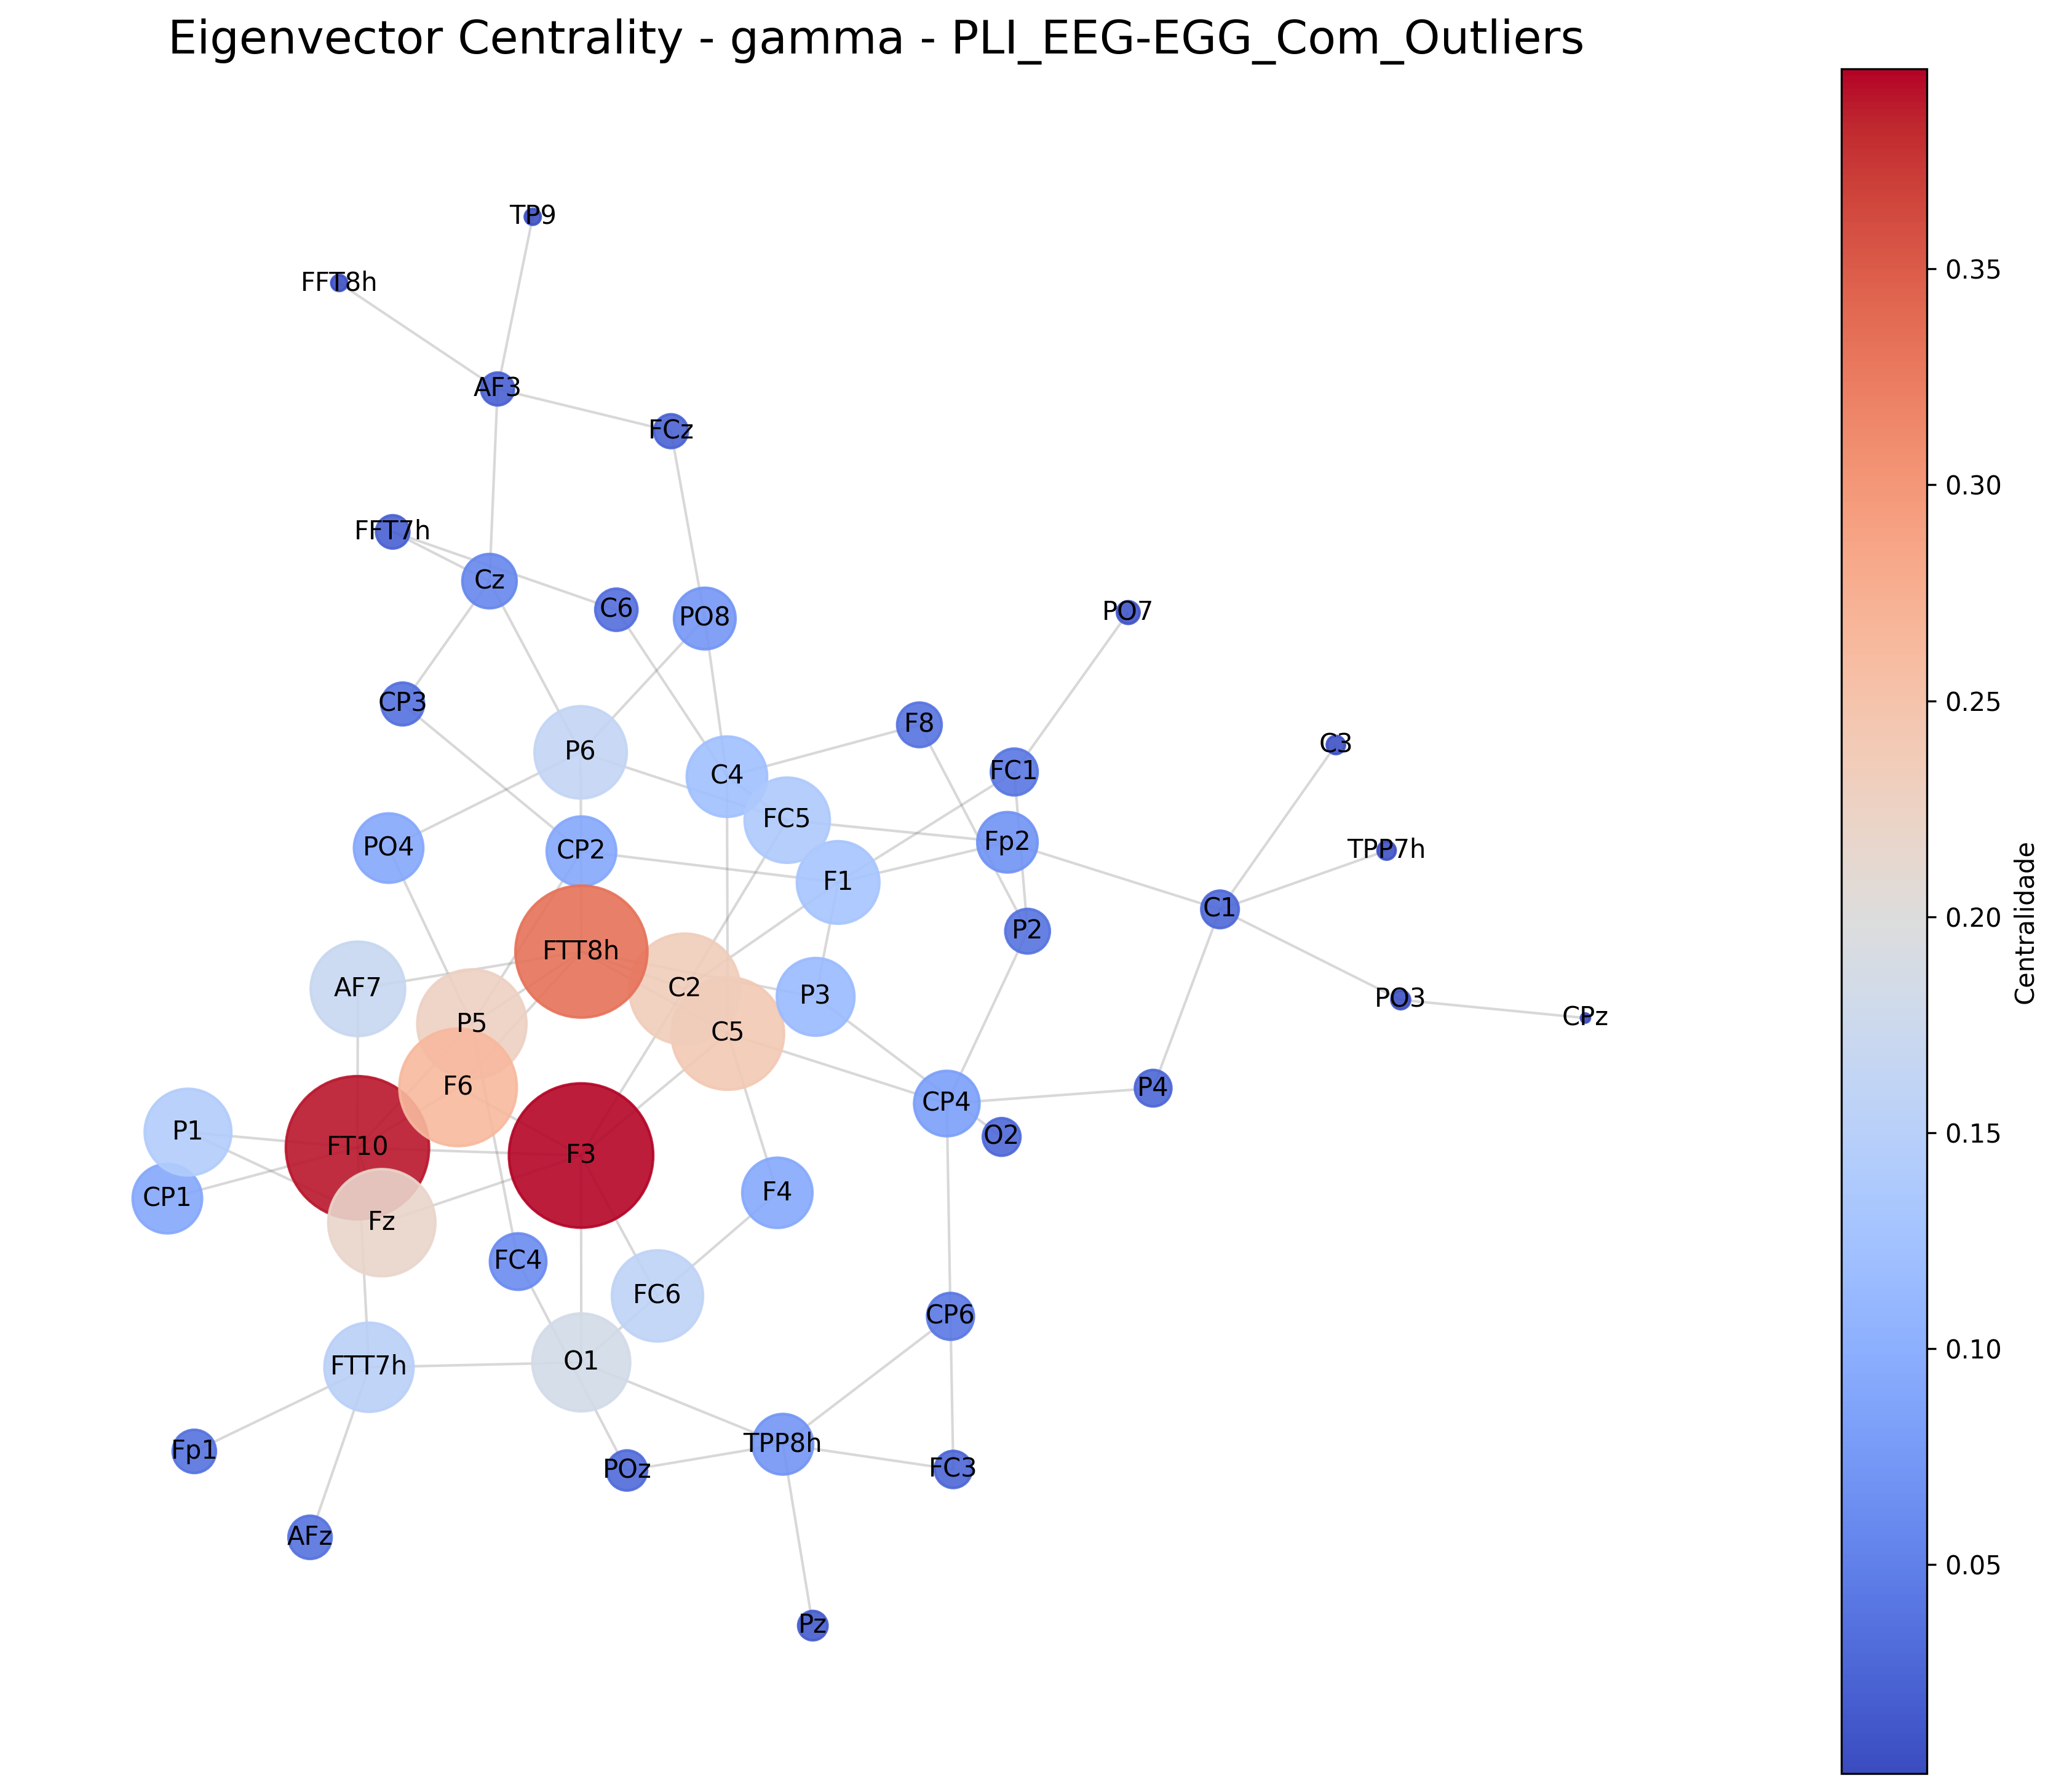
\includegraphics[width=0.45\textwidth]{figs/7_bootstrap_results_analysis/3_centrality_graphs/Com_Outliers/Eigenvector_Centrality__gamma__PLI_EEGEGG_Com_Outliers.png}
    }
    \hfill
    \subfloat[\small \textbf{Sem Outliers:} Hierarquia – 1. \textbf{FTT8h, C5, FT10}; 2. \textbf{F3}; 3. \textbf{P5}; 4. \textbf{AF7}; 5. \textbf{C2}.]{%
        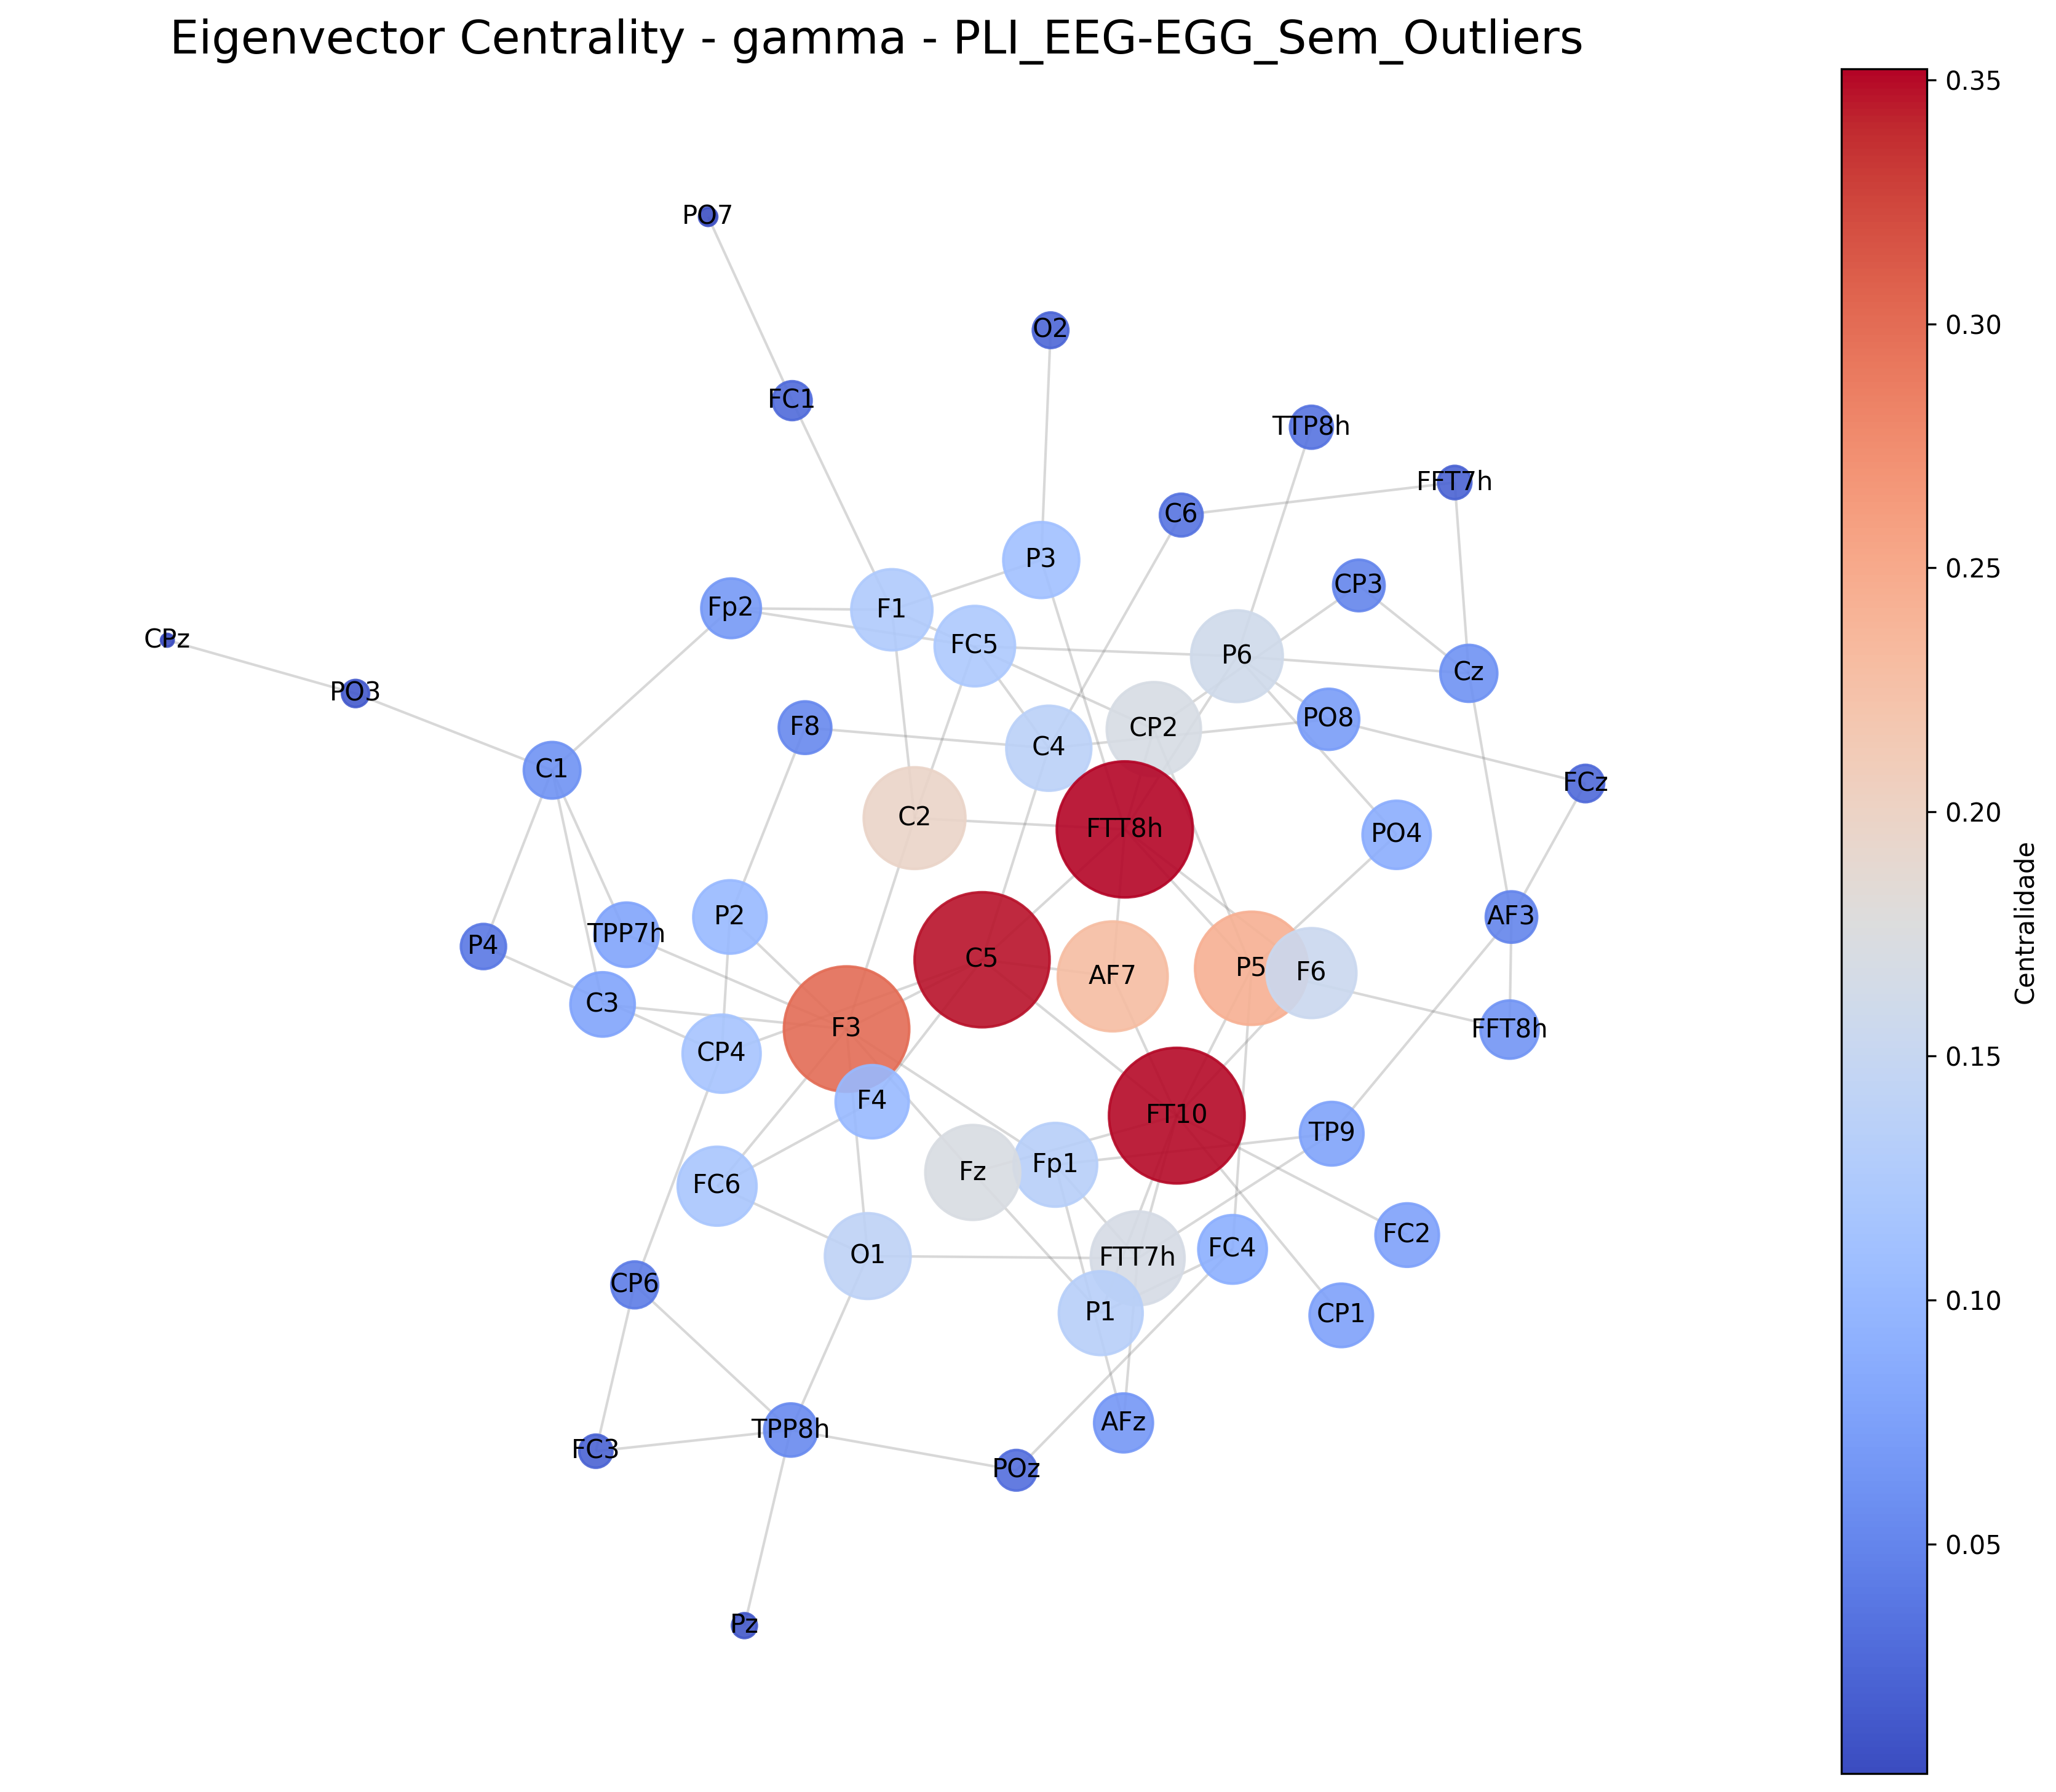
\includegraphics[width=0.45\textwidth]{figs/7_bootstrap_results_analysis/3_centrality_graphs/Sem_Outliers/Eigenvector_Centrality__gamma__PLI_EEGEGG_Sem_Outliers.png}
    }
    \caption{\small \textbf{Eigenvector Centrality – Banda Gamma (30--60 Hz):} A influência dos canais na rede gamma apresenta uma leve reorganização após a remoção dos outliers.}
    \label{fig:eigenvector_gamma}
\end{figure}

\subsection{Banda Theta (4--8 Hz)}

\subsubsection{Betweenness Centrality}
\begin{figure}[H]
    \centering
    \subfloat[\small \textbf{Com Outliers:} Hierarquia – 1. \textbf{FC1, PO4}; 2. \textbf{F8}; 3. \textbf{Fp2}; 4. \textbf{CP3, C1}.]{%
        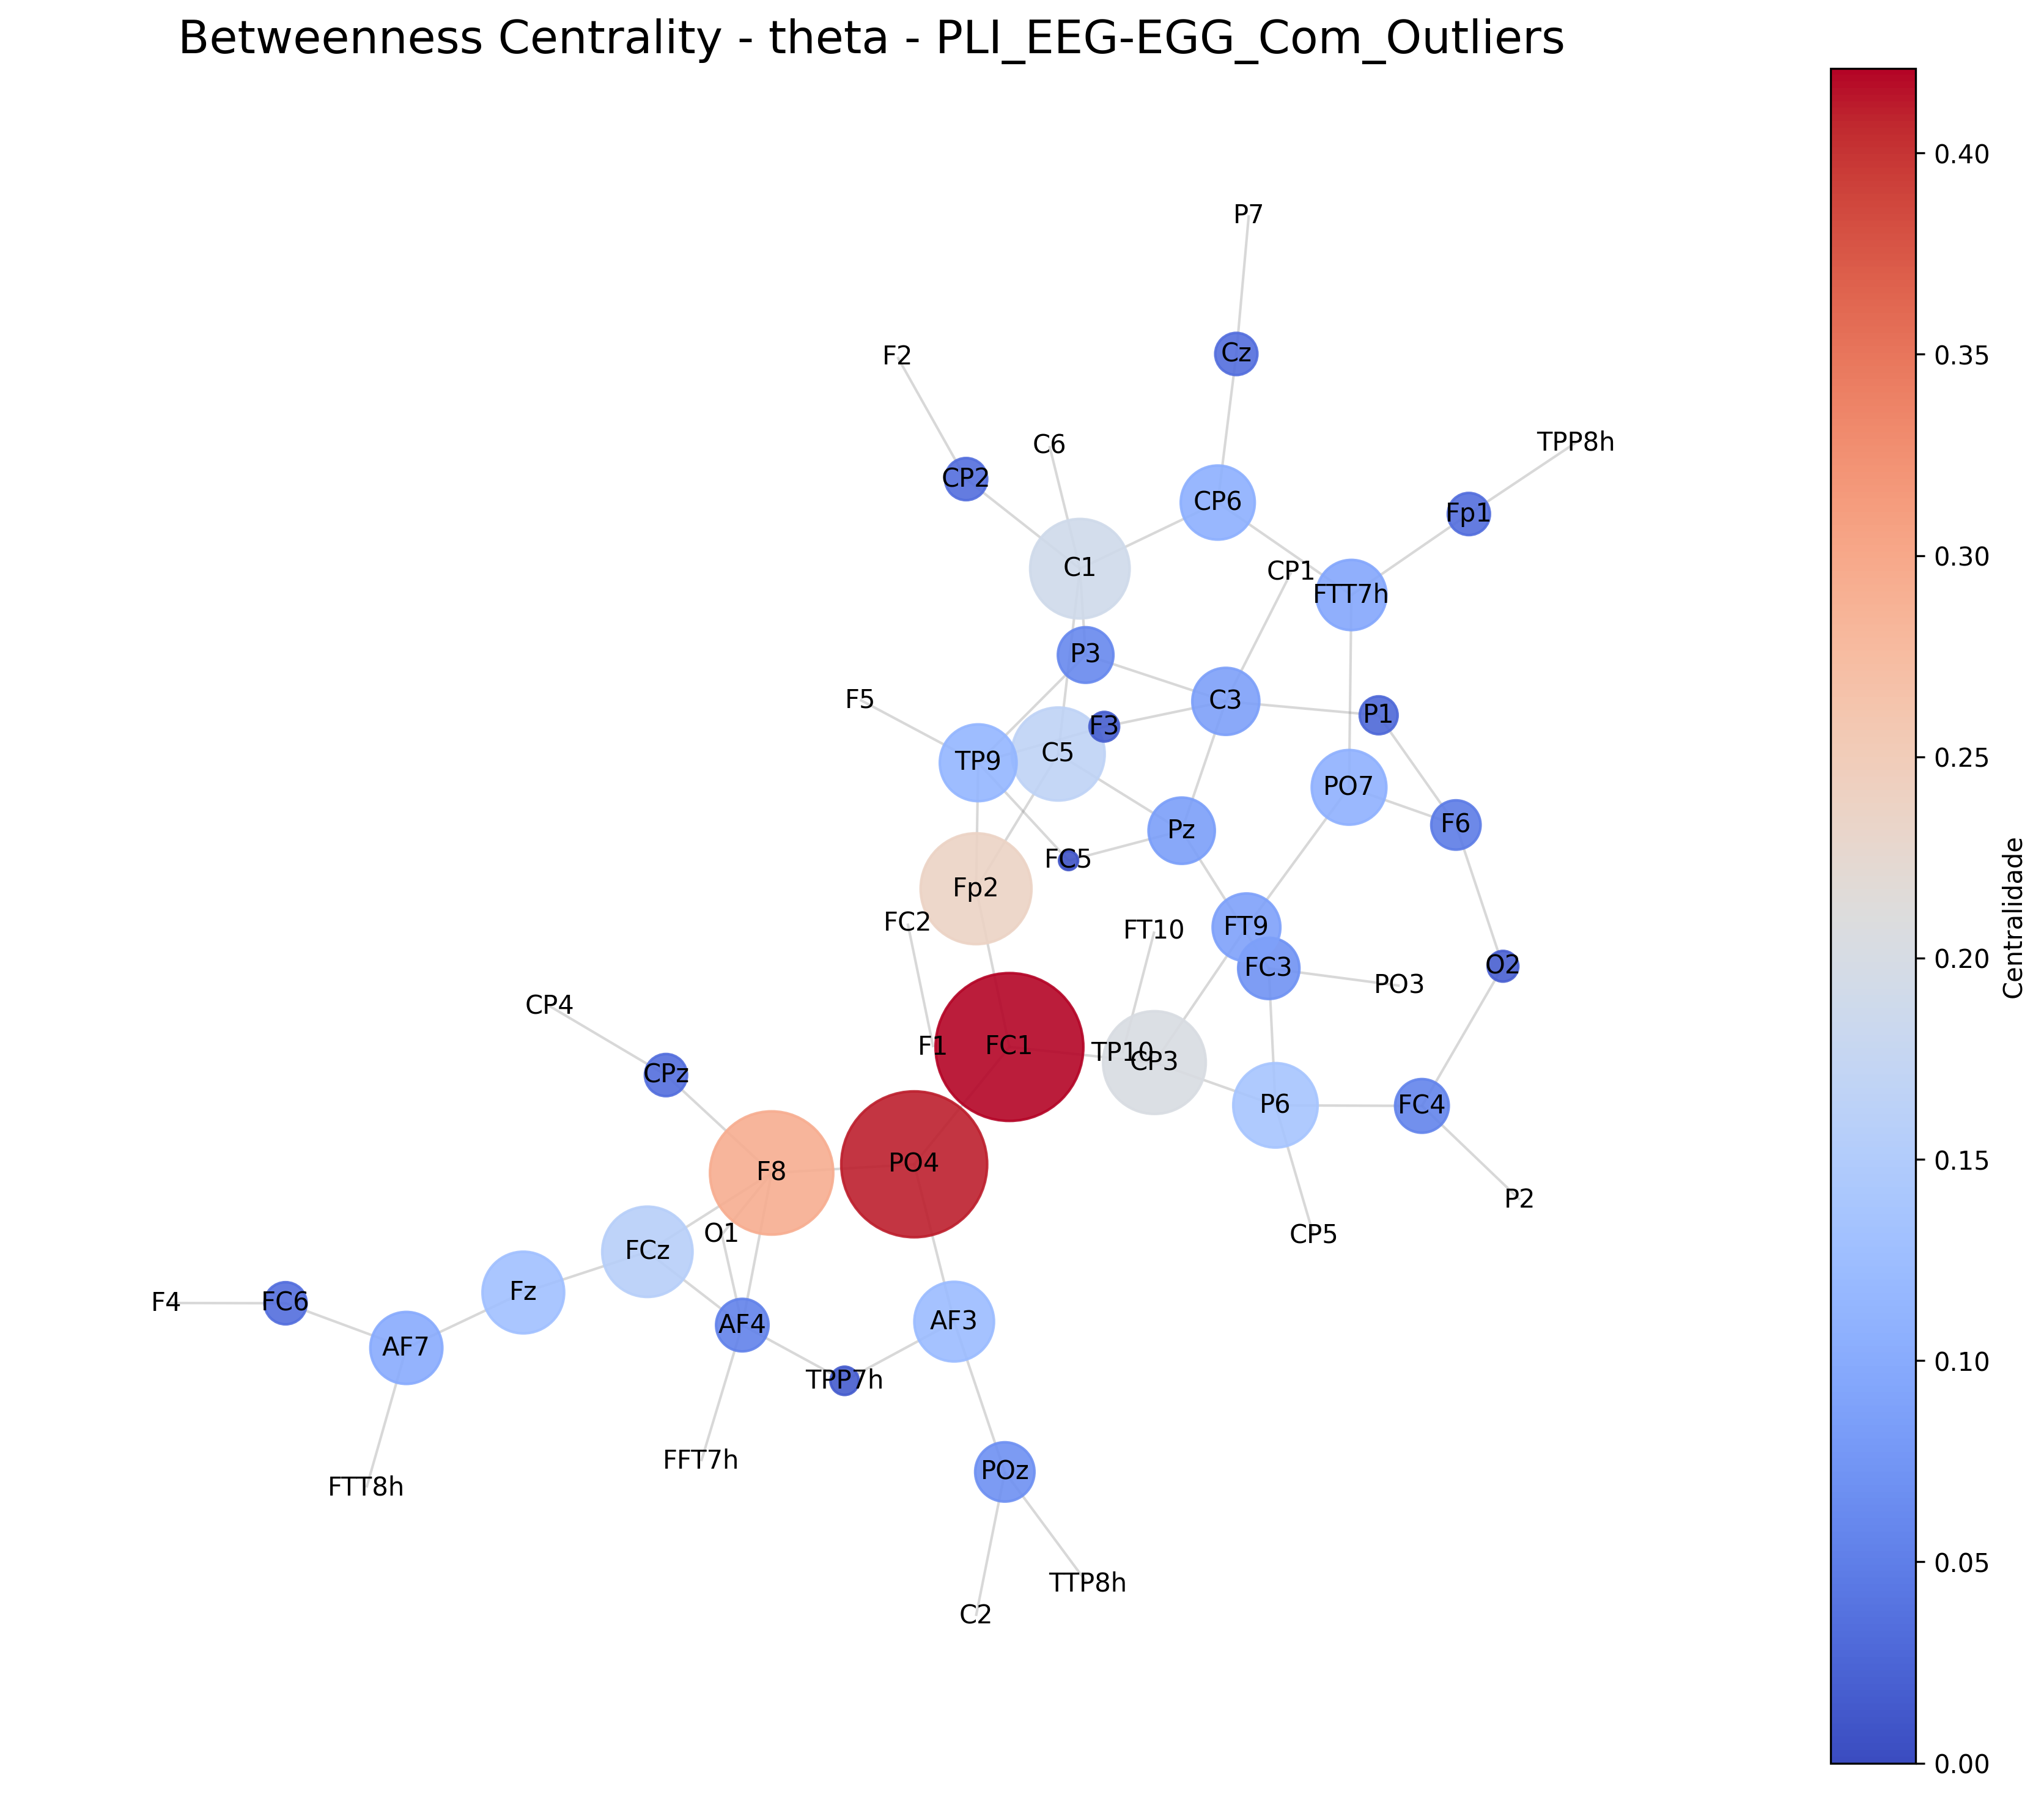
\includegraphics[width=0.45\textwidth]{figs/7_bootstrap_results_analysis/3_centrality_graphs/Com_Outliers/Betweenness_Centrality__theta__PLI_EEGEGG_Com_Outliers.png}
    }
    \hfill
    \subfloat[\small \textbf{Sem Outliers:} Hierarquia – 1. \textbf{PO4}; 2. \textbf{FC1}; 3. \textbf{C5, PO7, P7}; 4. \textbf{F8, AF3, Fp2}.]{%
        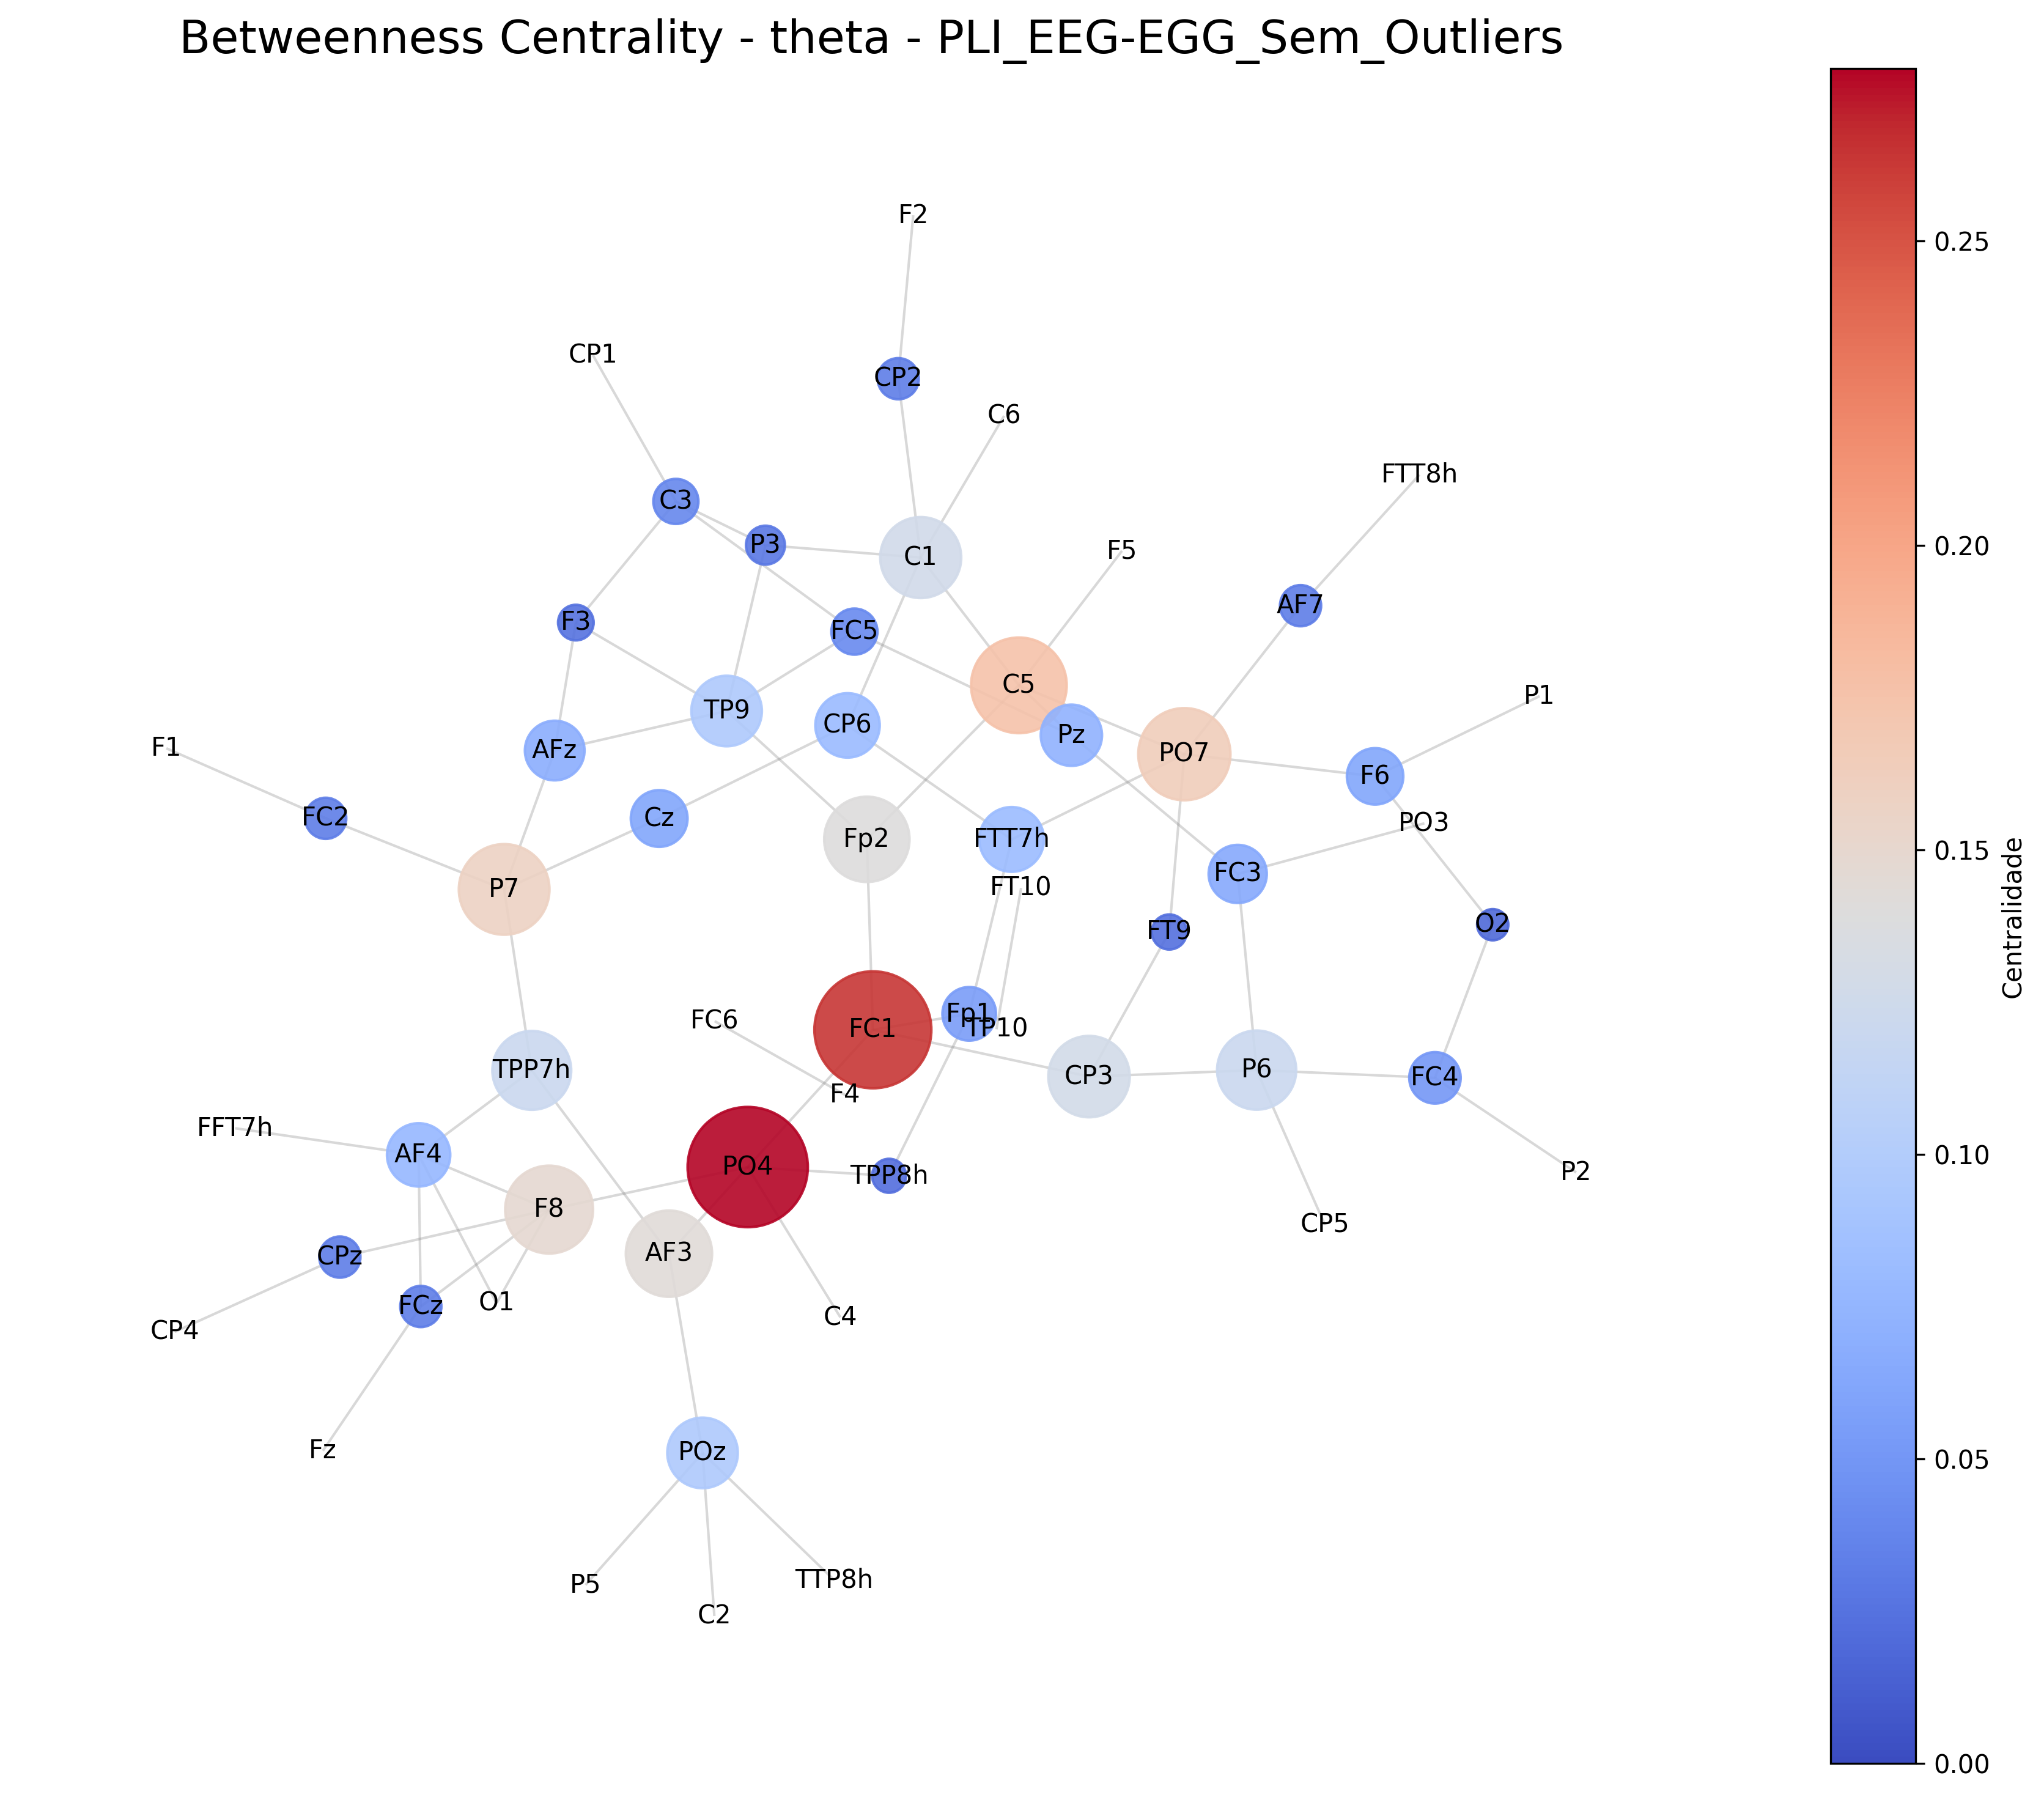
\includegraphics[width=0.45\textwidth]{figs/7_bootstrap_results_analysis/3_centrality_graphs/Sem_Outliers/Betweenness_Centrality__theta__PLI_EEGEGG_Sem_Outliers.png}
    }
    \caption{\small \textbf{Betweenness Centrality – Banda Theta (4--8 Hz):} A rede theta evidencia diferenças sutis na mediação dos caminhos, com reorganização da hierarquia após a remoção dos outliers.}
    \label{fig:betweenness_theta}
\end{figure}

\subsubsection{Degree Centrality}
\begin{figure}[H]
    \centering
    \subfloat[\small \textbf{Com Outliers:} Hierarquia – 1. \textbf{C1, C3, TP9, F8, AF4}; 2. \textbf{Pz, P6}.]{%
        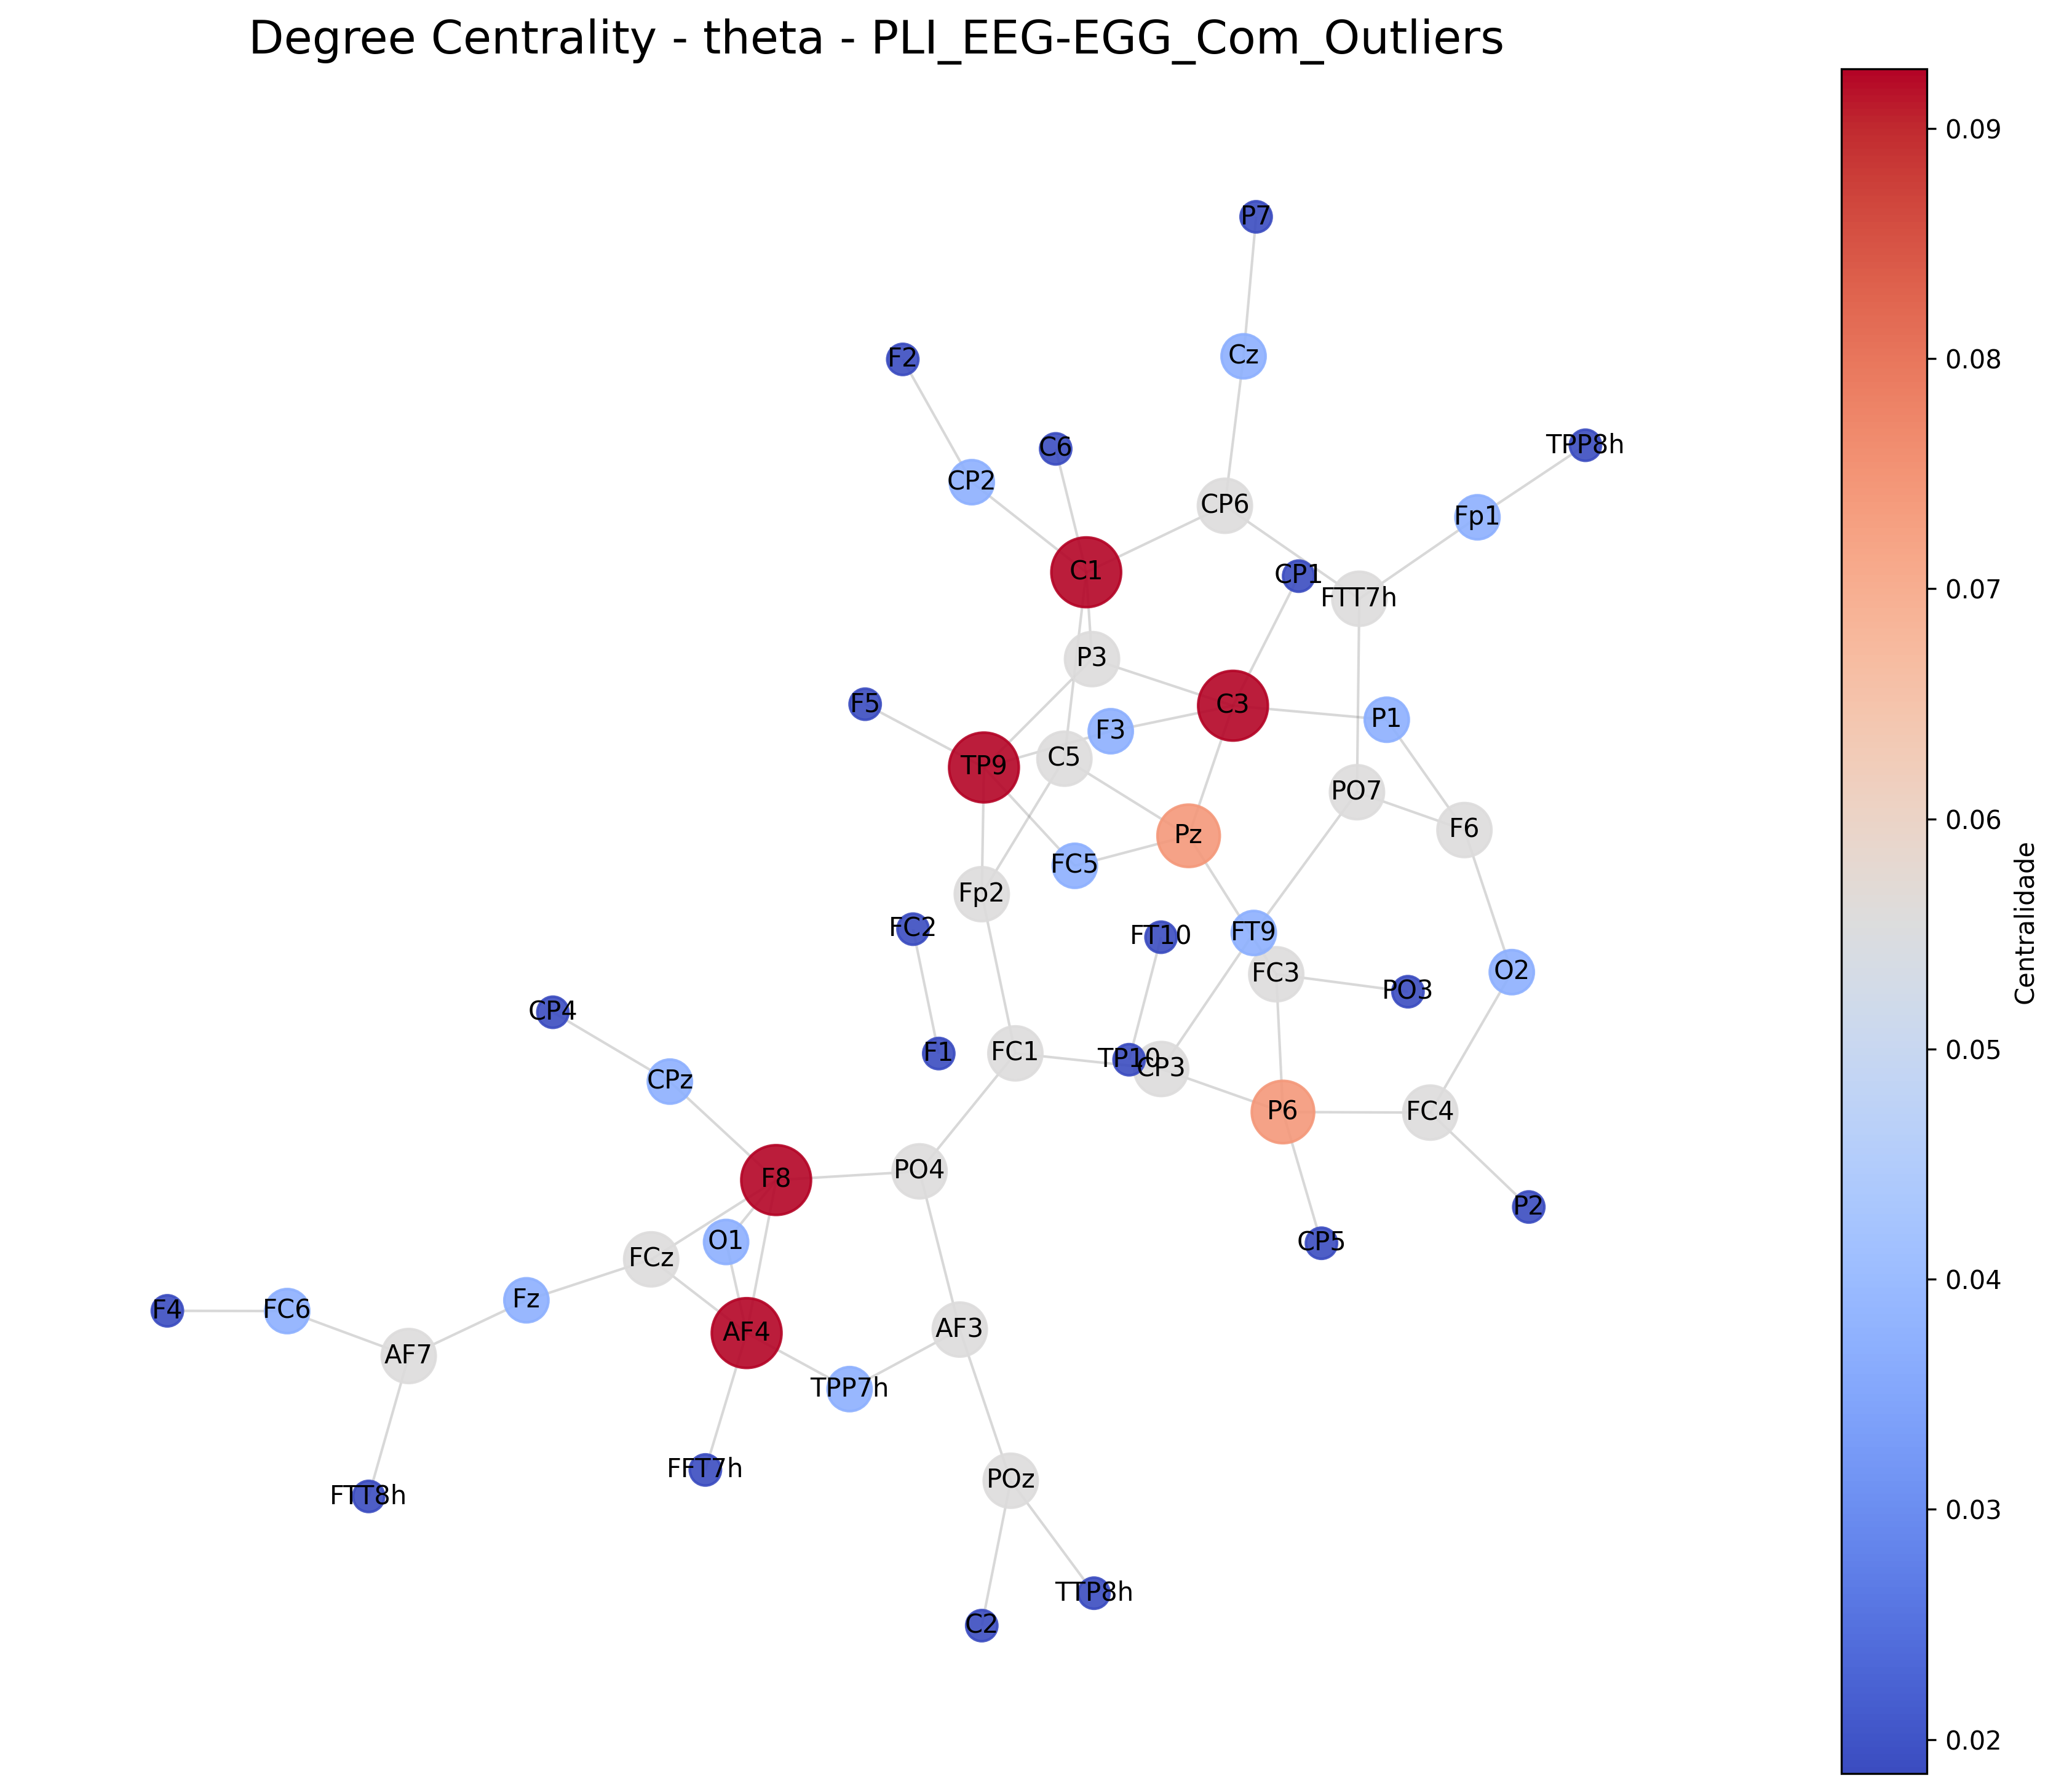
\includegraphics[width=0.45\textwidth]{figs/7_bootstrap_results_analysis/3_centrality_graphs/Com_Outliers/Degree_Centrality__theta__PLI_EEGEGG_Com_Outliers.png}
    }
    \hfill
    \subfloat[\small \textbf{Sem Outliers:} Hierarquia – 1. \textbf{C1, C5, TP9, PO7, PO4, F8, AF4}; 2. \textbf{POz, P7, FC1, P6, C3}.]{%
        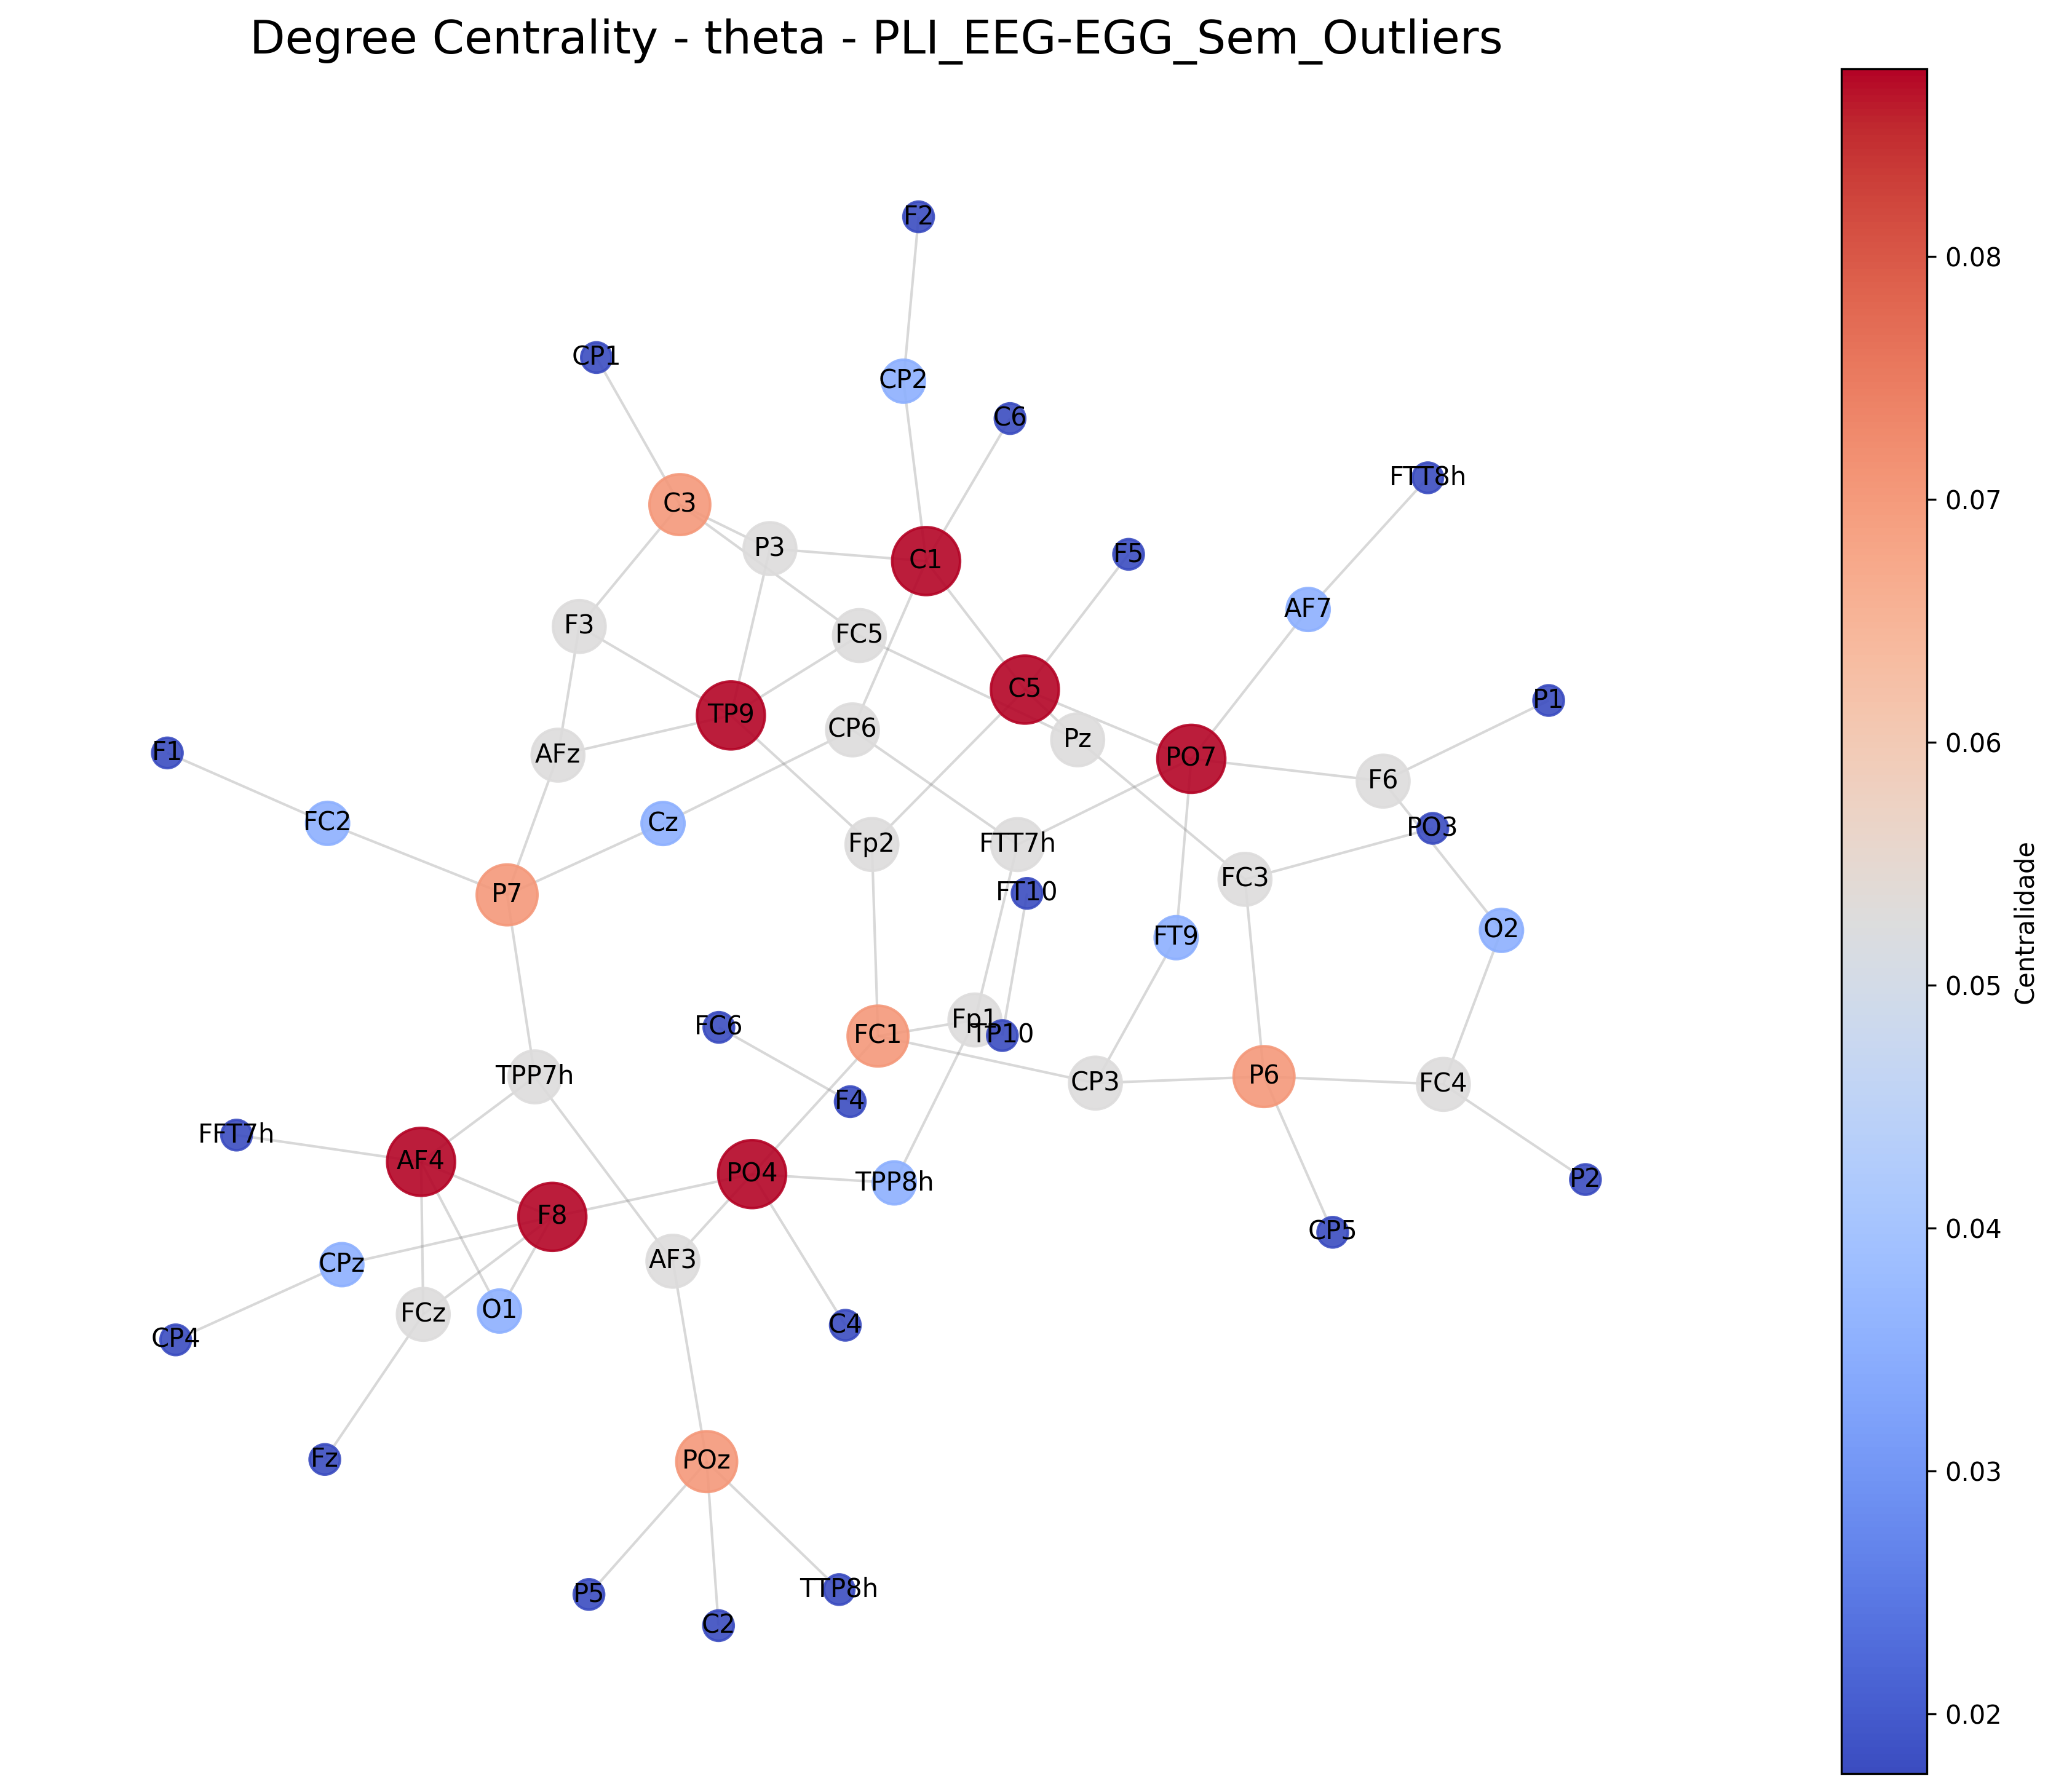
\includegraphics[width=0.45\textwidth]{figs/7_bootstrap_results_analysis/3_centrality_graphs/Sem_Outliers/Degree_Centrality__theta__PLI_EEGEGG_Sem_Outliers.png}
    }
    \caption{\small \textbf{Degree Centrality – Banda Theta (4--8 Hz):} A disposição dos canais na rede theta demonstra uma clara divisão entre nodos de alta e baixa conectividade, com leve reorganização após a remoção de outliers.}
    \label{fig:degree_theta}
\end{figure}

\subsubsection{Eigenvector Centrality}
\begin{figure}[H]
    \centering
    \subfloat[\small \textbf{Com Outliers:} Hierarquia – 1. \textbf{F8}; 2. \textbf{AF4}; 3. \textbf{FCz}; 4. \textbf{O1}; 5. \textbf{PO4, TP9}.]{%
        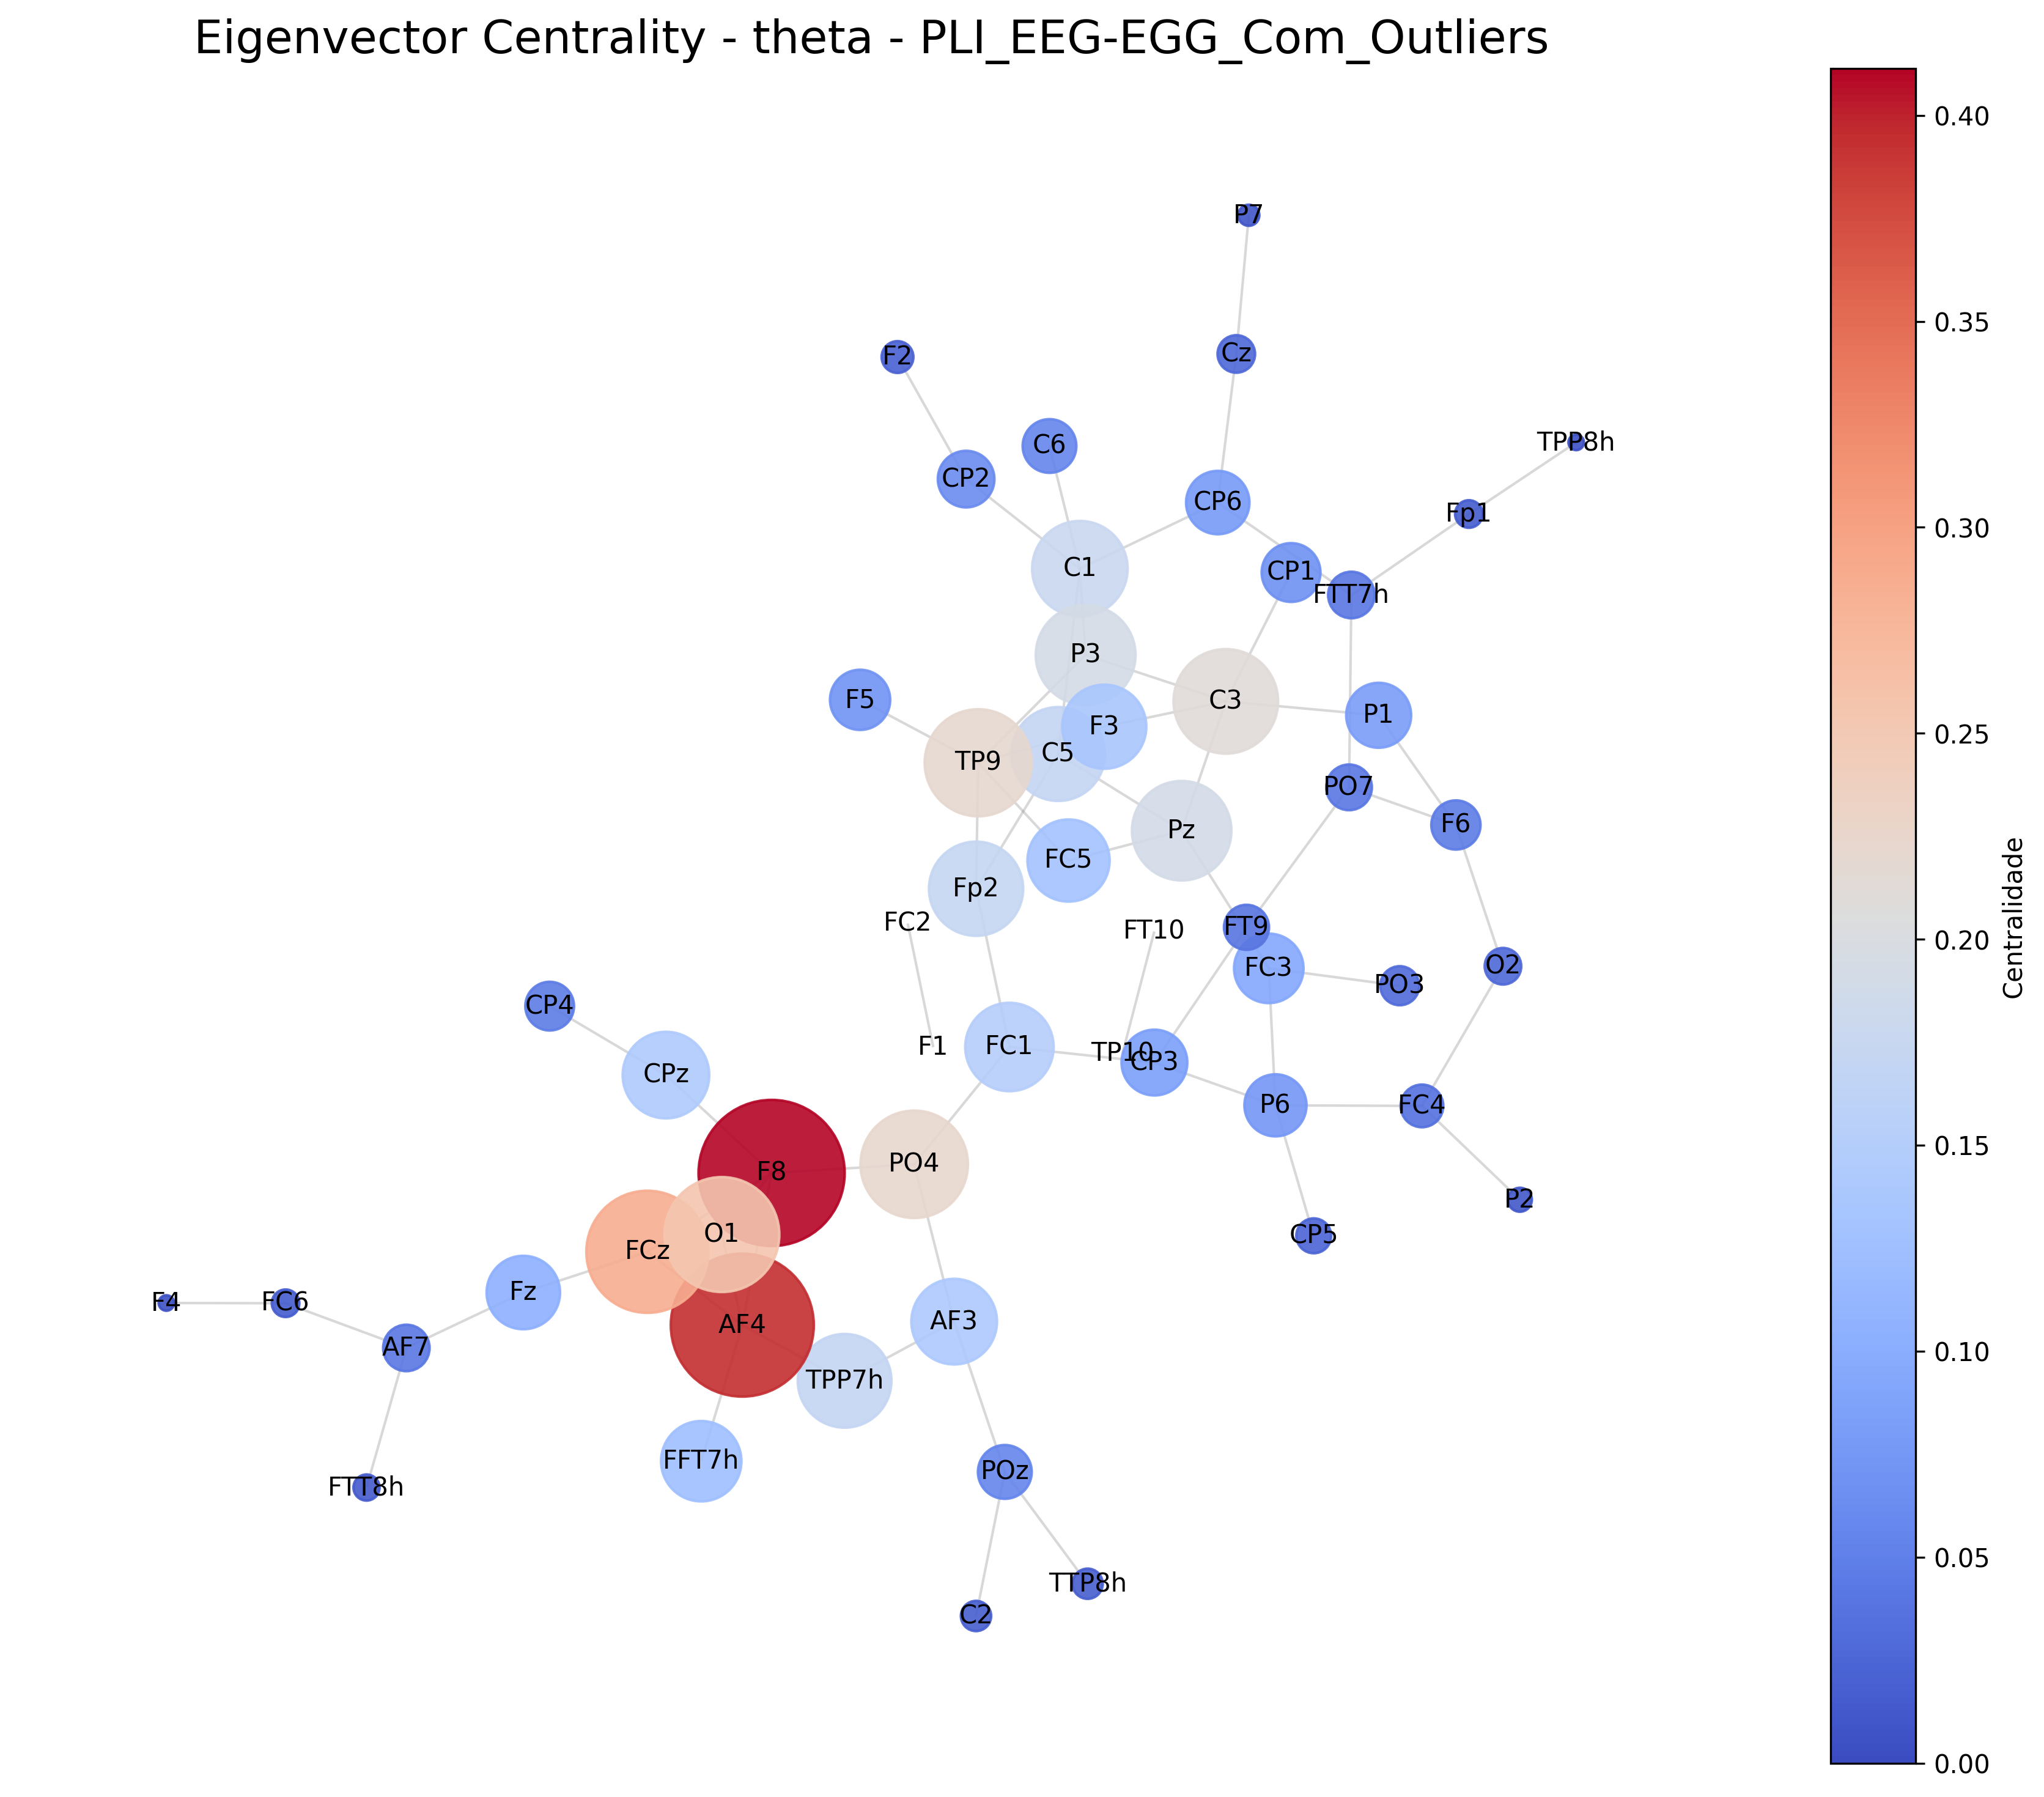
\includegraphics[width=0.45\textwidth]{figs/7_bootstrap_results_analysis/3_centrality_graphs/Com_Outliers/Eigenvector_Centrality__theta__PLI_EEGEGG_Com_Outliers.png}
    }
    \hfill
    \subfloat[\small \textbf{Sem Outliers:} Hierarquia – 1. \textbf{TP9}; 2. \textbf{C5}; 3. \textbf{Fp2, C1, P3, F3, F8, FC5, FC1, C3, AFz, AF4, PO4, FC1}.]{%
        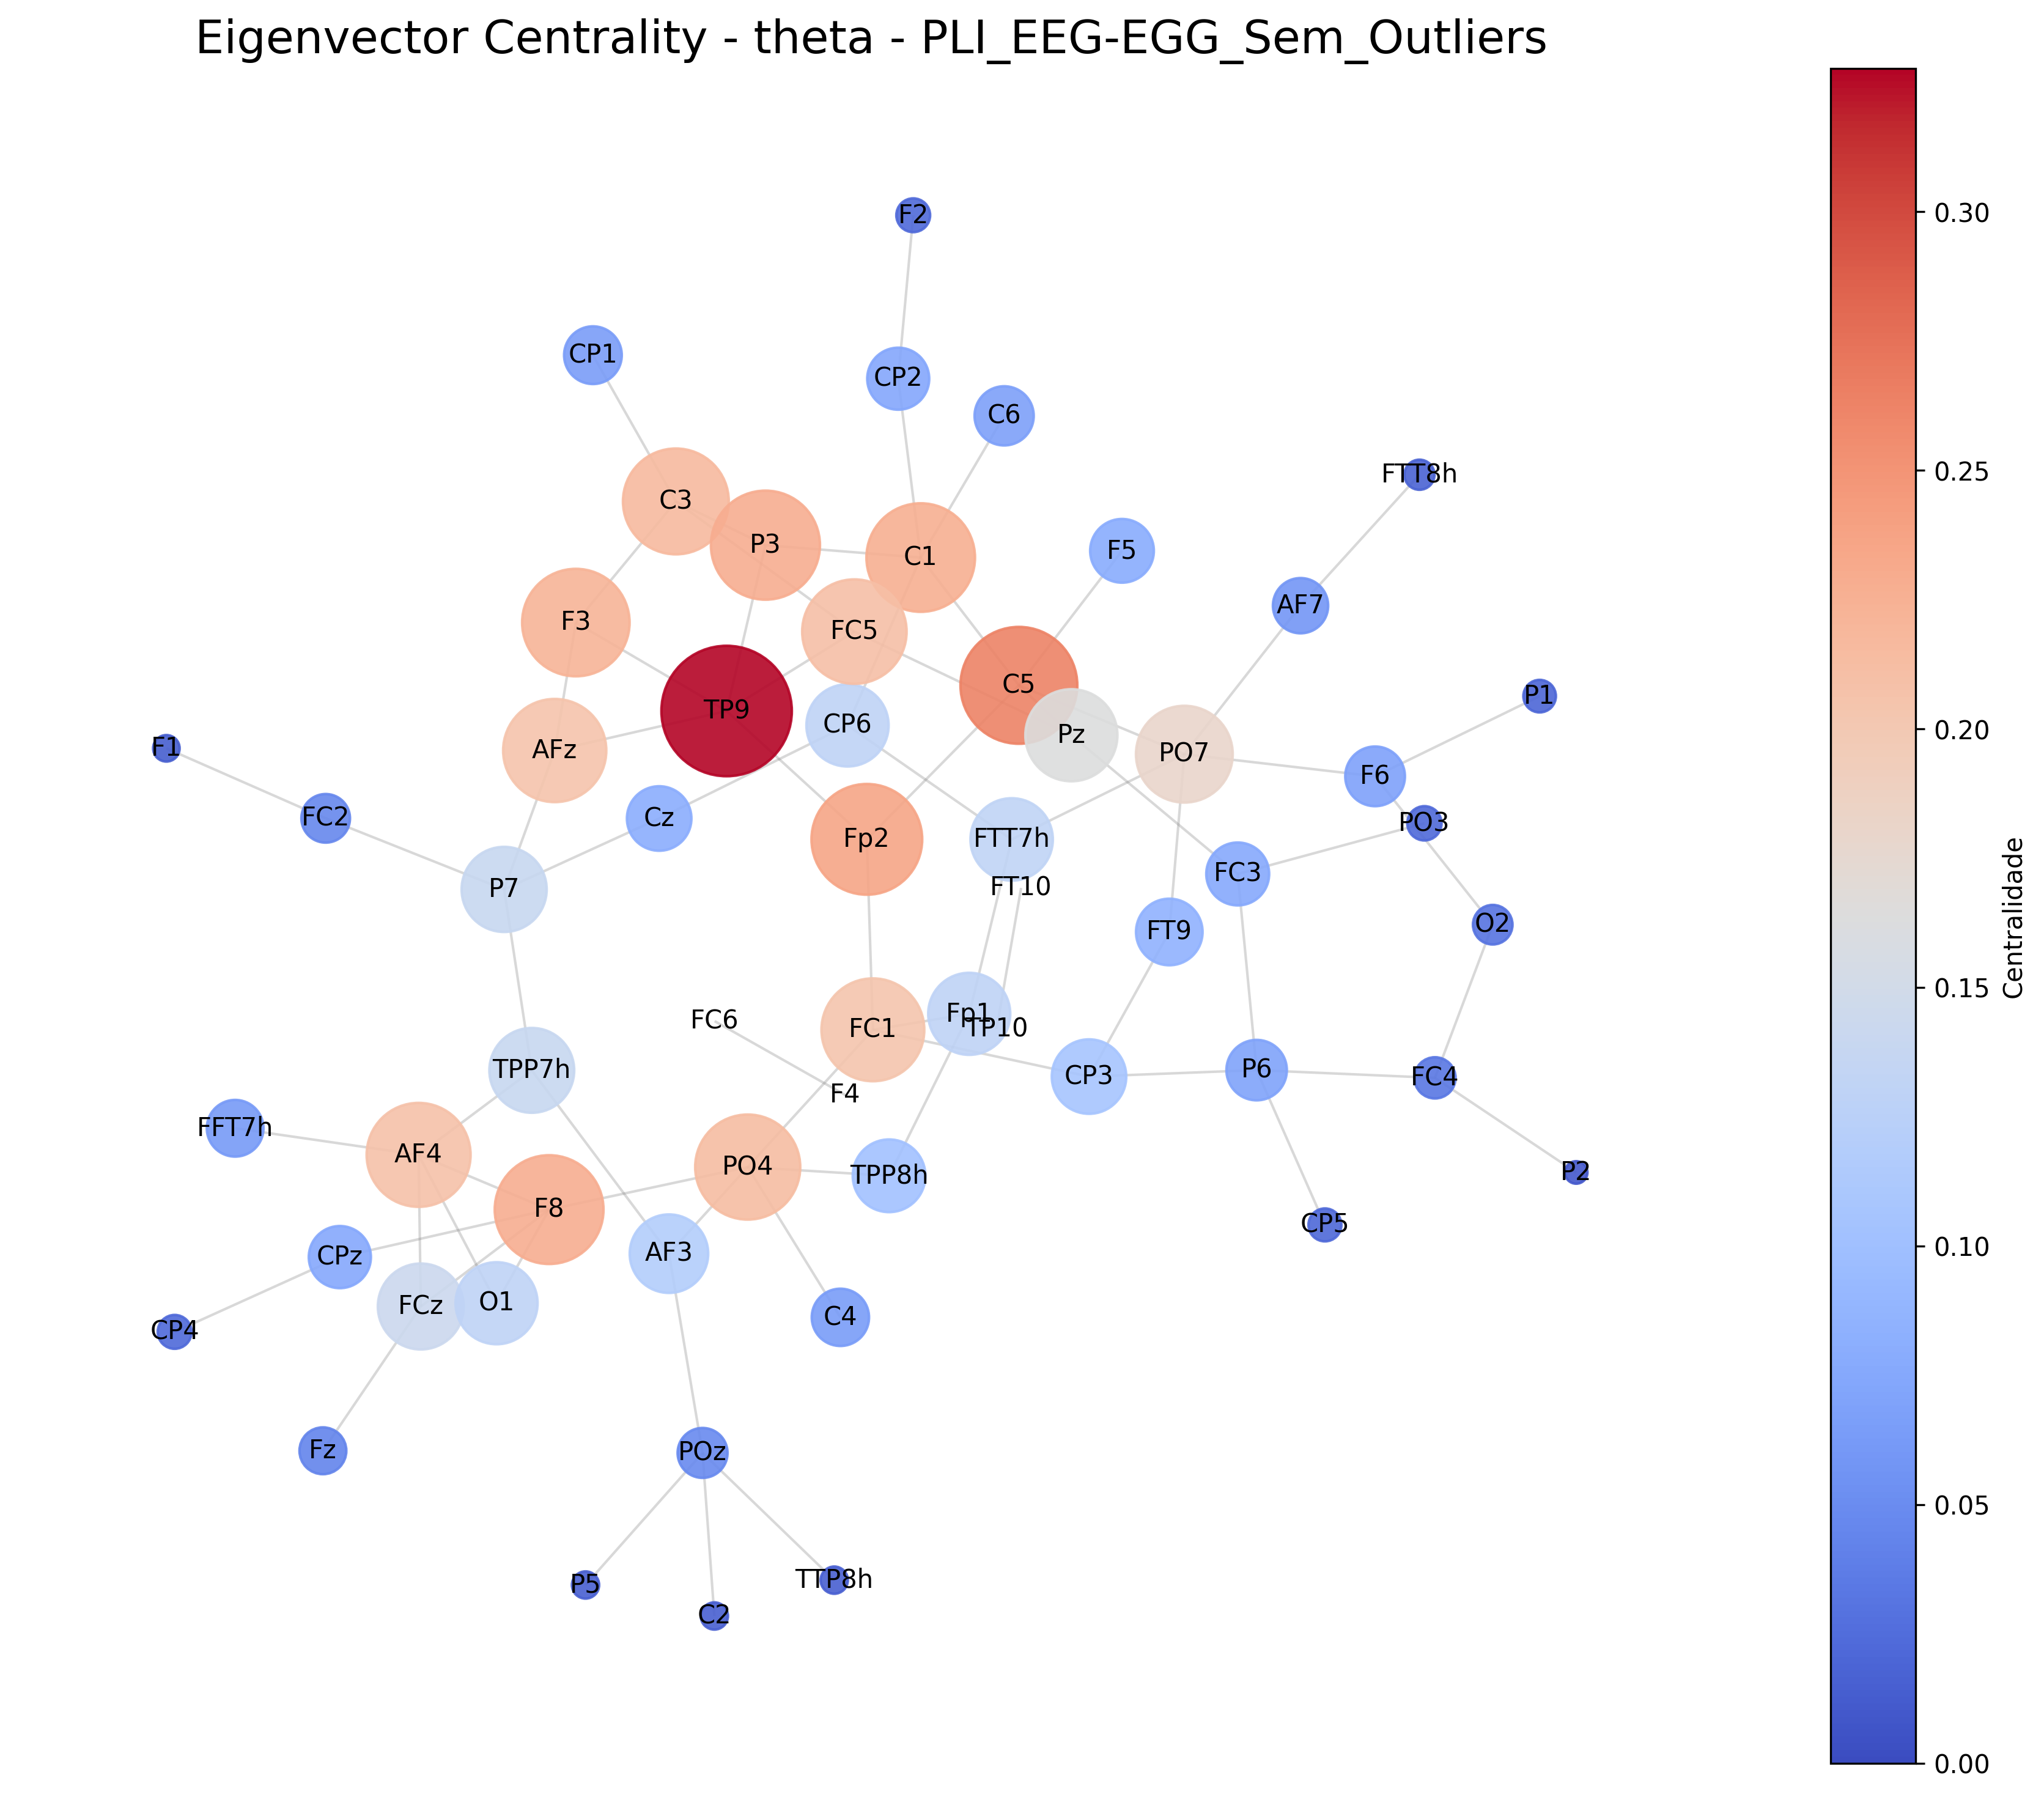
\includegraphics[width=0.45\textwidth]{figs/7_bootstrap_results_analysis/3_centrality_graphs/Sem_Outliers/Eigenvector_Centrality__theta__PLI_EEGEGG_Sem_Outliers.png}
    }
    \caption{\small \textbf{Eigenvector Centrality – Banda Theta (4--8 Hz):} As figuras evidenciam a hierarquia de influência na rede theta, com reorganização mais evidente na versão sem outliers.}
    \label{fig:eigenvector_theta}
\end{figure}

\section{Considerações Finais sobre a Centralidade de Grafos}

Os gráficos de centralidade apresentados evidenciam a hierarquia dos canais na rede de conectividade EEG–EEG (obtida via PLI). Em todas as métricas, os nós com maior centralidade – indicados por cores mais intensas (vermelho) e maiores tamanhos – correspondem a canais que atuam como hubs ou pontos-chave na rede. 

Observa-se que:
\begin{itemize}
    \item \textbf{Exibição dos Dados:} Apenas os casos de PLI EEG–EEG foram apresentados, uma vez que a análise de CF‐PLM (EEG–ECG) não fornece uma hierarquia diferenciada entre canais, dado que o ECG aparece em todas as conexões.
    \item \textbf{Hierarquia e Distribuição:} Em cada banda, os canais mais relevantes são listados em ordem decrescente de centralidade. Por exemplo, na banda Alpha, o canal \textbf{Fp2} é consistentemente o mais central, seguido por grupos de canais como \textbf{PO8}, \textbf{FC3} e outros, com pequenas variações entre os cenários com e sem outliers. Em bandas como Beta e Gamma, determinados canais (por exemplo, \textbf{TPP7h} na banda Beta e \textbf{FT10} na banda Gamma) se destacam como hubs principais.
    \item \textbf{Impacto da Remoção de Outliers:} Embora a remoção de outliers gere ajustes nos valores absolutos de centralidade e, consequentemente, na ordem intermediária dos canais, a estrutura global da rede se mantém similar entre os cenários. Em alguns casos, a hierarquia se reorganiza, como na banda Delta, onde a remoção de outliers desloca a centralidade de canais frontais (como \textbf{Fp2}) para canais parietais (\textbf{CP5} e \textbf{CP4}).
    \item \textbf{Padrões entre Bandas:} As bandas Alpha e Theta tendem a apresentar elevados valores de centralidade, refletindo uma maior integração e influência dos nós nessas frequências. Em contraste, a banda Delta exibe uma hierarquia mais sensível à presença de outliers, enquanto nas bandas Beta e Gamma certos canais se destacam de forma consistente.
\end{itemize}

Essas observações contribuem para a compreensão dos efeitos da neuromodulação na dinâmica da conectividade neural, destacando a importância dos canais em diferentes bandas de frequência e demonstrando a robustez dos achados mesmo após a remoção de outliers.
